\documentclass[a4paper,hidelinks,11pt]{memoir}
\usepackage[utf8]{inputenc} % Do not change or remove!
\usepackage[T1]{fontenc} % Do not change or remove
\usepackage[danish]{babel} % Sproget, vi skriver på
\renewcommand\danishhyphenmins{22} % Kun hvis vi skriver på dansk

%%%%%%%%%%%%%%%%%%%%%%%%%%%%%%%%%%%%%%%%%%%%%%%%%%%%%
% Niels Jakob Søe Loft                              %
% nsl@phys.au.dk                                    %
%%%%%%%%%%%%%%%%%%%%%%%%%%%%%%%%%%%%%%%%%%%%%%%%%%%%%

% Denne skabelon er baseret på Rasmus Villemoes' veldokumenterede
% phd-afhandling i matematik, som jeg har ændret på, så den passer til
% et bachelorprojekt i fysik. Som hovedregel er ting kommenteret på
% engelsk fra Rasmus' skabelon, mens jeg har skrevet på dansk. De
% væsentligste ændringer er, at skabelonen er gjort mere egnet til et
% mindre projekt som et bachelorprojekt er i forhold til en
% phd-afhandling, hvorfor nogle ting er skåret væk, og jeg har
% inkluderet en liste fysik-relaterede makroer. Desuden er
% bibliografien konverteret fra BibTeX til BibLateX pr. marts 2014.

% Pr. 29. marts 2014 har jeg ændret skabelonen, så den kan bruges til
% kompendiet til UNFs Fysik Camp 2014.

%%%%%%%%%%%%%%
%% Generelt %%
%%%%%%%%%%%%%%
% ***************** UNF Science camp  kompendie ***************** %
% Dette dokument indeholder enviroments, comannds, makroer og
% layot specifikt til UNF science camp kompendier

% Pakker der anvendes. Kendte 'issues:
%	- xcolor skal loades før pdfpages, da den ellers loades uden dvipsnames
\usepackage[dvipsnames]{xcolor}		% Farver
\usepackage{xparse}							% Mere flexibel definition af makroer
\usepackage{marginnote}					% Noter i margen
\usepackage{forloop}						% Mulighed for forløkker



% ***************** Opgave enviroment ***************** %
% Sætter en opgave op og angiver sværhedsgraden. Opgavenummereringen nulstilles
% efter hvert ny kapitel.
% Anvenedelse: 
%		\begin{opgave}[farve]{Titel}{Sværhedgrad}
%			Introduktion
%			\opg
%			Delopgave 1
%			\opg
%			Delopgave 2
%			...
%		\end{opgave}
%
% Definer selve enviromentet. i´
\newcounter{opgave}[chapter]
\newcounter{delOpgave}[opgave]
\newenvironment{opgave}[3][NavyBlue]
	{\newcommand{\opg}{{{\refstepcounter{delOpgave}\smallskip\newline\textbf\thedelOpgave})\,}}
	\noindent\ignorespaces\refstepcounter{opgave}\newline\textbf{Opgave \theopgave:\,#3 #2}\newline}
	{\newline\bigskip}
% Definer 
%\newcommand{\lvl}[2][NavyBlue]{
%	\setcounter{nBullets}{#2}
%	\addtocounter{nBullets}{1}
%	\checkoddpage
%	\ifoddpages
%		\normalmarginpar
%		\marginnote{\textcolor{#1}{\lvltoken{\value{nBullets}}}}
%	\else
%		\reversemarginpar
%		\marginnote{\textcolor{#1}{\lvltoken{\value{nBullets}}}}
%	\fi
%}
\NewDocumentCommand{\lvl}{ O{NavyBlue} O{$ \bullet $} m}{
	\setcounter{nBullets}{#3}
	\addtocounter{nBullets}{1}
	\checkoddpage
	\ifoddpage
	\normalmarginpar
	{\textcolor{#1}{\lvltoken[#2]{\value{nBullets}}}}
	\else
	\reversemarginpar
	{\textcolor{#1}{\lvltoken[#2]{\value{nBullets}}}}
	\fi
}
\newcounter{lvl}
\newcounter{nBullets}
\newcommand{\lvltoken}[2][$ \bullet $]{
	\forloop{lvl}{1}{\value{lvl} < #2}{#1}} % load UNF-layout
\usepackage{graphicx} % Billeder
\usepackage{epstopdf} % Så vi kan indsætte eps-filer
\usepackage{lipsum} % Dummytekst
\usepackage{pdfpages} % Indsættelse af pdf-sider
\usepackage{url} % Håndtering af URL'er
\usepackage{xspace} % Smarte mellemrum i egne makroer
\usepackage[final]{fixme} % Indsæt kommentarer i margin
%\usepackage{xstring} % Til sværhedsgrad-makro (se old/macros)
\usepackage[misc]{ifsym} % Til sværhedsgrad, skriv \Cube{n} hvor n=1,2,3
\usepackage{newtxtext}
\usepackage{newtxmath}
\usepackage{subcaption} %sub-figurer
\usepackage{framed} % tekst-bokse
\usepackage{wrapfig}
\usepackage{enumitem}
\usepackage{microtype} % Mellemrumsjustering
\usepackage{xcolor} % flere farver
\usepackage{tikz} % tegninger i latex
\usepackage{empheq}
\usetikzlibrary{decorations.pathmorphing,patterns} % til tikz
\usetikzlibrary{calc}

%% Bibliografi og referencer

%\usepackage{natbib} % Til biblografi, hvis man IKKE bruger BibLaTeX

%\usepackage[style=alphabetic,  % alternativt: style=numeric
%            backend=biber]{biblatex} % BibLaTeX, kræver installering
                                % af biber-pakken
%\addbibresource{kompendie.bib} % BibLaTeX tager referencer fra bach.bib

%\usepackage{cleveref} % Smarte referencer: skriv \cref{...}
\usepackage[colorlinks=true, hidelinks]{hyperref} % Farvede links

%%%%%%%%%%%%%%%%%%%%%%
%% Tekst og formler %%
%%%%%%%%%%%%%%%%%%%%%%

%\usepackage[osf]{mathpazo} % Skrift

\usepackage{wasysym} % Font til smileys \smiley og \frownie

%\usepackage[sf]{libertine} % Til slanted skrift NJ's emacs er pigesur
\usepackage{libertine}

\linespread{1.06} % Større linjeafstand pga. font
\usepackage{fourier-orns} % Sjove symboler NJ's emacs er pigesur igen
\usepackage{textcomp} % Tilføjer flere tegn
\renewcommand\ttdefault{txtt} % Pænere teletype-skrift

\usepackage{mathtools} % Matematiktricks
\usepackage{cancel} % Ting der går ud med hinanden
\usepackage{siunitx} %SI-enheder
\sisetup{separate-uncertainty=true % gør at siunitx skriver +/- i
  % stedet for at bruge parentes til
  % at angive usikkerheder.
  ,output-decimal-marker={,}, % gør at der bruges komma til komma og
  % ikke punktum som i USA.
  ,load=abbr, % så vi kan bruge \keV
  ,exponent-product = \cdot, output-product = \cdot, % skift gangetegn fra \times til \cdot
}
%% VI LAVER NOGLE FYSIK- OG MATEMATIK-MAKROER:


%% Generelt
%\newcommand{\g}{\cdot} % Prikprodukt, gangetegn
\newcommand{\subv}[2]{\gv{#1}_{\text{#2}}} % Pæn subscript til vektorer
\newcommand{\sub}[2]{#1_{\text{#2}}} % Pæn subscript til
\newcommand{\e}{\mathcal{E}} % Skrevet E
\newcommand{\abs}[1]{\left| #1 \right|} % Numerisk værdi
\newcommand{\N}{\ensuremath{\mathbb{N}}} % Naturlige tal
\newcommand{\Z}{\ensuremath{\mathbb{Z}}} % Hele tal
\newcommand{\Q}{\ensuremath{\mathbb{Q}}} % Rationelle tal
\newcommand{\R}{\ensuremath{\mathbb{R}}} % Reelle tal
\newcommand{\C}{\ensuremath{\mathbb{C}}} % Komplekse tal
\newcommand{\F}{\ensuremath{\mathbb{F}}} % Legeme tal
\newcommand{\A}{\ensuremath{\mathbb{A}}} % Algebraiske tal

%% Angiv sværhedsgrad til opgaver (benytter \usepackage{xstring})
%\newcommand{\lvl}[1]{%
%\IfStrEqCase{#1}{{1}{\ensuremath{\star}}
%    {2}{\ensuremath{\star\star}}
%    {3}{\ensuremath{\star\star\star}}}
%    [nada]
%}

%% Infinitesimalregning

\let\underdot=\d % omdøb indbygget kommando \d{} til \underdot{}
%\renewcommand{\d}[2]{\partial_{#2} \, #1} % afledt
%\newcommand{\dd}[2]{\partial_{#2}^2 \, #1} % dbl.afledt

%differentierings d
\renewcommand{\d}{\mathrm{d}}

%haard differentiering
\newcommand{\dif}[3][]{\frac{\d^{#1}{#3}}{{\d {#2}}^{#1}}}

%partiel differentiering
\newcommand{\pdif}[3][]{\frac{\partial^{#1}{#3}}{\partial {#2}^{#1}}}

\newcommand{\dt}[1]{\dot{#1}} % afledt mht. t (dot-notation)
\newcommand{\ddt}[1]{\ddot{#1}} % dbl.afledt mht. t (dbl.dot)

\newcommand{\integral}[4]{\int_{#3}^{#4} \, #1 \, \textrm{d}#2} % integrere



% Vektorer

\newcommand{\xyz}[3]{\begin{bmatrix} #1 \\ #2 \\ #3 \end{bmatrix}} %3D-vektor
\newcommand{\xy}[2]{\begin{bmatrix} #1 \\ #2 \end{bmatrix}} %2D-vektor
\let\vaccent=\v % Omdøb \v{} til \vaccent{}

\newcommand{\gv}[1]{{\vec{\mathbf{#1}}}} % Vektor med græske bogstaver
\renewcommand{\v}[1]{\gv{#1}} % Vektor med fed
\newcommand{\hatvec}[1]{\hat{\mathbf{#1}}} % Hatvektor
\newcommand{\ihat}{\boldsymbol{\hat{\textbf{\i}}}} % Enhedsvektor i
\newcommand{\jhat}{\boldsymbol{\hat{\textbf{\j}}}} % .. j
\newcommand{\khat}{\mathbf{\hat{k}}}  % .. k
\newcommand{\xhat}{\mathbf{\hat{x}}} % Enhedsvektor x
\newcommand{\yhat}{\mathbf{\hat{y}}} % .. y
\newcommand{\zhat}{\mathbf{\hat{z}}} % .. z
\newcommand{\grad}[1]{\gv{\nabla} #1} % Gradient
\let\divsymb=\div % Omdøb \div til \divsymb
\renewcommand{\div}[1]{\gv{\nabla} \cdot \v{#1}} % Divergens
\newcommand{\curl}[1]{\gv{\nabla} \times \v{#1}} % Curl
% Vil man tage div eller curl af græske bogstaver,
% skal man lade argumentetet være fx \gv{\mu} for µ-vektor

% Kvantemekanik

\newcommand{\op}[1]{\hat #1} % operator

\newcommand{\expect}[1]{\left< #1 \right>} % Forventningsværdi
\newcommand{\trace}{\ensuremath{\text{Tr}}\xspace}
\newcommand{\Hilbert}{\ensuremath{\mathcal{H}}}
\newcommand{\lag}{\ensuremath{{L}}}
\newcommand{\tr}[1]{\text{Tr}\left(#1\right)} % Trace
\newcommand{\ptr}[2]{\text{Tr}_{#1}\left(#2\right)} % Partial trace
\newcommand{\ket}[1]{\left| #1 \right>} % Dirac-notation: ket
\newcommand{\bra}[1]{\left< #1 \right|} % bra
\newcommand{\braket}[2]{\left< #1 \vphantom{#2} \, \right|
  \left. \! #2 \vphantom{#1} \right>} % bracket
\newcommand{\matrixel}[3]{\left< #1 \vphantom{#2#3} \right|
  #2 \left| #3 \vphantom{#1#2} \right>} % Bracket med ekstra streg
 % En masse matematik- og fysikmakroer

%%%%%%%%%%%%
%% Layout %%
%%%%%%%%%%%%

\newcommand{\anonbreak}{\fancybreak{$* * *$}} % Break med stjerner
\let\bar\overline % Gør at en bar over et symbol kan skalere efter symbolet

%% Sidehoved- og fod

\makepagestyle{tket}
\makeevenfoot{tket}{\thepage}{}{}
\makeoddfoot{tket}{}{}{\thepage}
\makeevenfoot{plain}{\thepage}{}{}
\makeoddfoot{plain}{}{}{\thepage}
\pagestyle{tket}

%% Margin

% Man kan sætte margins ved enten at specificere marginstørrelsen
% eller ved at specificere tekstblokken. Man skal vælge én og kun én
% af mulighederne.

% Specificer marginstørrelsen
%\setulmarginsandblock{2.7cm}{*}{1}
%\setlrmarginsandblock{1.6cm}{1.6cm}{*} 
%\setlength{\oddsidemargin}{-1cm} % Giver mere plads på siden
%\setlength{\topmargin}{-1.2cm} % Gør topmargin behagelig at se på
%\setlength{\columnsep}{1.5\columnsep}  % Afstand mellem søjlerne


\setlrmarginsandblock{2.5cm}{2.5cm}{*}

\usepackage[font={small,it}]{caption}	% Italic captions

% Tekstblok: Følgende er fra Rasmus Villemoes' thesis-layout.tex
%\setlxvchars[\normalfont] % standardbredden af tekstblok er ca. 65 tegn
%\settypeblocksize{*}{1.2\lxvchars}{1.61803} % højde, bredde, forhold
%\setulmargins{*}{*}{1.3} % lav bundmargin lidt større end topmargin
\checkandfixthelayout % memoir tjekker, at alt er ok og konsistent

%%%%%%%%%%%%%%%%%%
%% Definitioner %%
%%%%%%%%%%%%%%%%%%

% Definer titlen på projektet
 \newcommand{\thesistitle}{Kompendie til UNF Fysik Camp 2017}

%%%%%%%%%%%%%%%%%%%%%%
%% Slut på preamble %%
%%%%%%%%%%%%%%%%%%%%%%


%%%%%%%%%%%%%%%%%%%%%% 
%%  BEGIN DOCUMENT  %%
%%%%%%%%%%%%%%%%%%%%%%


\begin{document}

\frontmatter
% The titlingpage environment used in frontstuff resets the page
% numbering to start at 1 at the end. But this means that several
% pages will be known as i, ii, iii (since the \frontmatter sets
% \pagenumbering{roman}). This is not a problem in print, since the
% first few pages don't have folios. But hyperref will complain about
% "destination with the same identifier (name{page.i})". To avoid
% these, we pretend that the first few pages are numbered with
% uppercase roman letters...
\pagenumbering{Roman}

\include{old/frontstuff} % forside og kolofon

\clearpage
% ... and remember to reactivate the lowercase numbering.
\pagenumbering{roman}
\tableofcontents

\chapter{Introduktion}
\label{cha:introduktion}

Velkommen til UNF Fysik Camp 2017. Dette kompendium er en introduktion
til de emner, som vi skal arbejde med i løbet af campen. Programmet,
som I skal igennem, indeholder flere forskellige emner, som alle
giver et indblik i, hvor vigtig og alsidig fysikken er. Emnerne er i år laserfysik, astrofysik, rotationel mekanik, relativitetsteori, elektromagnetiske bølger og kerne- og partikelfysik, hvor I blandt de sidste fire selv får lov til at vælge, hvilke to I ønsker at arbejde med. Alle er de relevante for vores verden, og vi håber, at I
vil finde dem lige så spændende, som vi selv gør.

I kommer alle med forskellig undervisningsbaggrund, og vi kræver
derfor ikke, at I bare forstår alt med det samme. Under campen vil der
være rig mulighed for at snakke mere om det, der står i dette
kompendie og virkelig dykke ned i stoffet. Kompendiet indeholder alt,
hvad I vil få brug for til at forstå og arbejde med emnerne under
campen, og I opfordres derfor kraftigt til at læse det. Særligt bør I
forsøge at læse de to første kapitler om laserfysik og astrofysik,
da disse emner vil indgå i det obligatoriske program, hvorimod de
andre emner er valgfrie.

Da I kommer fra forskellige klassetrin, har I ikke alle modtaget
undervisning i al den matematik, som I måske skal bruge. I opfordres
derfor også til at læse appendikset bagerst i kompendiet, som
forklarer den matematik, vi skal arbejde med på campen. Den relevante matematik for campens hovedemner er dækket i Afsnit A.2 og A.3, hvorfor disse er vigtigst at læse. 

God fornøjelse, og velkommen i fysikkens verden.

\begin{flushright}
På vegne af det faglige team, \\
\textit{Dorte Thrige Plauborg, fagligt ansvarlig } 
\end{flushright}

%%% Local Variables: 
%%% mode: latex
%%% TeX-master: "main"
%%% End: 

\mainmatter

%her sættes emner ind.

%Du begynder bare at skrive
\chapter{Astrofysik}
\section{Kosmologi}
Kosmologi er læren om universets skabelse, udvikling og endeligt. Når der snakkes om universets størrelse, er det normalt det synlige univers, der menes. Dette er den del af universet, hvor lys er nået hen til os, så vi kan observere det. Længere ude er informationen ikke nået frem til os endnu, så vi ved ikke, hvor stort hele universet er. 

Det stemmer overens med \emph{det kosmologiske princip}, der siger, at universets love og konstanter er ens overalt og massen er ligevægt fordelt (set fra en stor nok skala). Det kan deles op i to postulater: Universet er homogent (ens i hvert område) og isotropt (ser ens ud, uanset hvilken retning man kigger i), som illustreret i Figur \ref{isohomo}. Det kosmologiske princip behøver ikke gælde, men vi har ikke observeret noget, der bryder med det. Princippet antages derfor normalt at gælde, da det er det simpleste -- vi har ingen grund til at tro, at universets egenskaber pludselig ændrer sig et sted. Det er en god approksimation på skalaer fra 200 Mpc (megaparsec) og opefter. 1 pc er cirka 3 lysår, så det er $3\cdot 10^8$ lysår. På små skalaer holder det selvfølgelig ikke. For eksempel er du tættere (har større massefylde) end luften omkring dig, og Solen kan udpege en særlig retning inden for solsystemet.

Antagelsen om, at universet er homogent og isotropt, er understøttet af
kortlægningen af den \emph{kosmiske mikrobølgebaggrund} (eng: CMB – cosmic microwave
background). Baggrunden består af stråling fra det tidspunkt, hvor universet blev
gennemsigtigt (ca. 380 000 år efter Big Bang) – altså hvor temperaturen af plasmaet
og strålingen dannet efter Big Bang er aftaget tilstrækkeligt, så det er muligt for frie elektroner at 
kombinere med atomkerner og danne hydrogen og helium
og lyset kunne undslippe. Af historiske årsager kaldes dette for \emph{rekombinationen}, men man kalder det også for \emph{foton--afkoblingen}. Den kosmiske mikrobølgebaggrund er derfor det ældste
lys i universet! Dengang var strålingen i UV-området, men udvidelsen af Universet
(Afsnit \ref{12}) har nu kølet den til en temperatur på 2.73 K og flyttet den til mikrobølgeområdet. Den kosmiske mikrobølgebaggrund er blevet kortlagt af flere
missioner, først COBE (Cosmic Background Explorer), siden WMAP (Wilkinson
Microwave Anisotropy Probe) og senest Planck, se Figur \ref{CMB}. Det ses, at selv med høj opløsning er kortet uniformt – beviset på et næsten
homogent og isotropt tidligt univers. Men små fluktuationer i tætheden er stadig til
stede, og var det ikke for disse, ville den gravitationelle tiltrækning ikke have kunnet
skabt de galakser, vi observerer (og bebor!) i dag.

\begin{figure}[h]
	\centering
	\includegraphics[width=0.7\textwidth]{Astrofysik/Astrofig/CMB.jpg}
	\caption{Kortlægningen af den kosmiske mikrobølgebaggrund af COBE, WMAP og
		Planck. Mælkevejen, som ellers ville være til stede i billedet, er redigeret ud. }
	\label{CMB}
\end{figure}
%Fra http:
%		//www.planetastronomy.com/astronews/astrn-2013/04/astron3.jpg

\begin{figure}[h]
	\centering
	\includegraphics[width=0.7\textwidth]{Astrofysik/Astrofig/isohomo.png}
	\caption{Venstre: Illustration af isotropi. Fra midten ser verden ens ud i alle retninger. Højre: Illustration af homogenitet. Kigger man på et stort nok udsnit af verden, vil det se ud som alle andre udsnit.}
	\label{isohomo}
\end{figure}

%\section{Big Bang og CMB}
\section{Rødforskydning}
\label{12}
\subsection{Dopplerforskydning}
Du kender nok til, at når en ambulance kører forbi, så lyder sirenens tone højere når den nærmer sig, og dybere når den kører væk. Det skyldes \emph{Dopplerforskydning}. %Find gerne lydklip til undervisningen
Det skyldes, at lydbølgerne skubbes sammen og strækkes, afhængigt af hvilken fart de udsendes med i forhold til lytteren. Hvis en ambulance kører mod dig, og du står stille, vil du høre bølgerne sammenpresset. Men hvis du selv kører med samme hastighed foran ambulancen, så vil du høre dem på samme måde, som de bliver udsendt - altså på samme måde som hvis begge biler står stille, da det er den relative hastighed, som er afgørende.

\begin{figure}[h!]
	\centering
	\includegraphics[width=0.7\textwidth]{Astrofysik/Astrofig/doppler.jpg}
	\caption{Dopplerforskydning af lyden fra en bil, der kører mod venstre. Person A vil høre end højere tone end person B, og personen i bilen vil høre noget et sted derimellem. Ringene viser et fast punkt på lydbølgerne.}
	\label{shapes}
\end{figure}

Det samme sker for lys. Hvis en ambulance kører væk, vil både tonen blive dybere og lyset fra den en smule rødere. Bemærk dog, at selvom fotoner og lydbølger har højere energi ved korte bølgelængder, så mister de ikke energi ved Dopplerforskydning - der er bare sket et skift i perspektivet, man ser bølgerne fra. Fra bølgens eget synspunkt (hvis man følger den) har den samme bølgelængde og energi hele tiden.
\subsection{Kosmologisk Rødforskydning}
Edwin Hubble opdagede i 1920'erne, at galakser langt borte ser rødforskudte ud, men dette skyldes \emph{ikke} Dopplerforskydning fra galaksernes egenhastighed i forhold til os. Så ville vi have forventet, at lige så mange galakser var rødforskudte som blåforskudte, hvis de starter med en tilfældig hastighed. Og det gør de jo - for hvorfor skulle de have en særlig retning i forhold til os? Det ville bryde med isotropien. 

Hubble opdagede, at galakserne oftere er rødforskudt end blåforskudt, og jo længere væk de er, desto mere rødforskudte er de også. Han formulerede \emph{Hubbles lov}, der beskriver den direkte proportionalitet mellem afstand og fart af en galakse:
\begin{align}
v=H_0 D, \label{Hubbleslaw}
\end{align}
hvor $v$ er farten, $D$ er afstanden til galaksen, og $H_0=67.7\pm0.5$ er Hubbles konstant, som er den nuværende værdi af Hubble-parameteren (der ikke er konstant).

Galaksers relative hastighed til os er altså større, desto længere væk de er. Og sådan vil det se ud fra ethvert punkt i universet. Derfor må rødforskydningen stamme fra, at alting bevæger sig længere væk fra hinanden, som rosiner i en hævende bolle. Det er netop, hvad der sker - universets dej dvs. selve rumtiden "hæver". Galakserne har lige ofte egenhastigheder der går mod os som fra os, men hastigheden, som selve rumtiden udvider sig med, er vigtigere for galakser langt væk. For fjerne galakser skal lyset bevæge sig gennem mere rum for at nå frem til os. Derfor når lyset at blive strukket mere end ved nære galakser. 

Ved rødforskydning fra universets udvidelse mister lyset rent faktisk energi i modsætning til almindelig Dopplerforskydning. Dette er selvfølgelig et brud på energibevarelse, men det er egentlig ikke et problem, da man ikke kan betragte universet som et lukket system, fordi det udvider sig. Energibevarelse behøver kun at gælde i lukkede systemer. Nogle mener dog, at ændringen i energi fra universets udvidelse (og den mørke energi der opstår, se afsnit \ref{bestanddele}) udlignes af, at den gravitationelle energi falder til endnu lavere negative niveauer, således at universets totale energi altid er 0.

Måden, man måler rødforskydningen på, er ved at opsplitte lyset i dets forskellige bølgelængder. Dvs. man tager spektrer af fjerne objekter, og derefter genkender man mønstre fra jordiske laboratorier. Niels Bohr opdagede, at elektroner kun kan eksistere i bestemte baner om en atomkerne, men ikke mellem disse. Hver bane har en bestemt energi, så elektronernes energi i atomer er kvantiseret, dvs. de findes kun i bestemte pakker. Når en elektron henfalder til en lavere tilstand, kommer den af med overskydende energi ved at udsende en foton. Og hvis en foton med passende energi rammer en elektron, kan fotonen blive absorberet, så elektronen kommer op i en højere energitilstand. 

For lysspektrer gælder 3 love kaldet Kirchoffs love (ikke at forveksle med Kirchoffs love for elektriske kredsløb), som er illustreret i Figur \ref{kirchoff}.
\begin{itemize}
	\item Varme, uigennemsigte objekter udsender lys kontinuert over hele spektret. Ideelt set ville det give spektret for sortlegemestråling, og det er en særligt god approksimation for varme stjerner. Mindre stjernes lys er mere "forurenet" af effekter fra molekylær hydrogen (det er relativt koldt) og andre stoffer.
	\item Varme, gennemsigte gasser udsender lys og danner emissionsspektrer.
	\item Kolde gasser danner absorptionslinjer. Hvis en stjerne ligger bagved og sender lys mod os, vil skyen absorbere lyset og udsende det senere i en tilfældig retning. Det er meget usandsynligt, at retningen er mod os igen, så vi ser mindre lys ved denne bølgelængde.
\end{itemize}

\begin{figure}[h]
	\centering
	\includegraphics[width=0.7\textwidth]{Astrofysik/Astrofig/kirchoffslaws.jpg}
	\caption{Kontinuert spektrum (til højre), absorptions-spektrum (midtfor) og
		emissions-spektrum (til venstre). }
	\label{kirchoff}
\end{figure}
%fra http://astro.psu.edu/public-outreach/fireworks-masks-1/absorption-and-emission-spectra

\begin{figure}[h!]
	\centering
	\includegraphics[width=0.7\textwidth]{Astrofysik/Astrofig/spektrum.png}
	\caption{Et typisk stjernespektrum. Y-aksen skal forstås som intensitet, mens der
		på X-aksen er bølgelængde i ångstrøm (Å) (1 Å = $10^{-10}$ m). Dykkene i intensitet
		er angivet med en overgang tilhørende et grundstof, som er identificeret i stjernens
		atmosfære. }
	\label{shapes}
\end{figure}
%fra http://i.stack.imgur.com/RMHmB.gif

Har man en galakse med en stjerne, som udsender et bredt spektrum af lys, vil lyset både bevæge sig gennem stjernens ydre "kolde" lag og galaksens gasskyer, før det når os. Stjerner og skyer består af forskellige stoffer såsom hydrogen. Når de belyses, absorberer hydrogenet fotoner med de energier, der svarer til energiforskellen mellem banerne i hydrogen. Der dannes derfor et helt bestemt mønster af absorbtionslinjer i spektret, som er unikt for f.eks. hydrogen. For en rødforskudt galakse vil mønsteret ligge ved længere bølgelængder, end det vi måler for hydrogen på Jorden, men det er stadig genkendeligt.

Når vi kan genkende et mønster af absorptionsliner eller emissionslinjer, selvom det ligger forskudt ved andre bølgelængder end normalt, så kan vi finde rødforskydningen. Den er defineret som forskellen mellem observeret bølgelængde $\lambda_{obs}$ og laboratoriebølgelængde $\lambda_{lab}$ i forhold til laboratoriebølgelængden. Det er altså den relative forskydning i forhold til den oprindelige bølge. Lad os opskrive det som

\begin{align}
z=\frac{\lambda_{obs}-\lambda_{lab}}{\lambda_{lab}}.
\end{align}
Rødforskydningen $z$ er relateret til farten $v$ således:
\begin{align}
z+1=\sqrt{\frac{1+\frac{v}{c}}{1-\frac{v}{c}}}.
\end{align}
For hastigheder meget langsommere end lysets hastighed i vakuum $c$, kan det forsimples til:
\begin{align}
z\approx\frac{v}{c}.
\end{align}

Rødforskydning er altså en form for afstandsmål, men også et tidsmål, da lyset har rejst i lang tid, hvis det har nået at passere en stor afstand og er blevet meget udtrukket. Hvordan rødforskydningen relaterer til andre måder at måle afstand afhænger af, hvordan rumtiden strækker lyset. Og det afgøres af Universets form via generel relativitetsteori.

\section{Universets Form}

Universet har samlet set en form. Vi har 3 tydelige rumdimensioner omkring os, og vi er vant til, at hvis man tegner to parallelle linjer, så vil de aldrig krydse, og en trekant har altid 180 grader. Men dette gælder kun i fladt rum! Forestil dig f.eks. en trekant tegnet på en globus; den vil faktisk have mere end 180 grader. På samme måde vil en trekant tegnet på en saddel have mindre end 180 grader, som på Figur \ref{shapes}. Hvis universet er kugleformet, har det en positiv krumning, og hvis det er saddelformet, har det en negativ krumning. I et fladt univers er krumningen 0.

\begin{figure}[h!]
	\centering
	\includegraphics[width=0.7\textwidth]{Astrofysik/Astrofig/universe_geometry.png}
	\caption{Trekanter i forskellige geometrier har forskellige vinkelsummer. }
	\label{shapes}
\end{figure}

Hvis et objekt er i frit fald, eller hvis man har en lysstråle, vil de bevæge sig langs en ret linje i rumtiden (kaldet en geodæt). Men hvis selve rumtiden krummer, så gør den "rette"  linje det også. Derfor kan man se universets krumning ved at kigge på lyset fra objekter langt væk. Den viser sig ved, om ting ser forstørrede eller formindskede ud (om strålerne spredes eller samles som i en linse), og disse målinger viser, at universet er fladt med en præcision på 0.5 \%. Det vender vi tilbage til i afsnit \ref{bestanddele}. %Kilde + illustration

Hvis universet var positivt krumt og småt nok, ville det også betyde, at lyset kunne nå hele vejen rundt, og vi ville se de samme objekter flere steder på himlen, hvilket heller ikke er observeret. Så det synlige univers er i hvert fald meget fladt -- men måske har rumtiden en svag krumning, der bare ikke kan ses her. Selvom Danmark ser fladt ud, kan hele jordkloden jo godt være rund.

Hvis universet er positivt krumt, er det endeligt, mens fladt eller negativt rum kan være uendeligt stort. Det er dog også muligt for universet både at være f.eks. fladt og endeligt, men så bryder man det kosmologiske princip.

Vi kan sammenligne universets størrelse ved forskellige tidspunkter gennem en skalafaktor $a(t)$. Vi definerer den nuværende faktor til 1, dvs. $a(t_0)=1$, hvor $t_0$ er tiden nu. Der gælder:
\begin{align}
\frac{a(t_0)}{a(t)}=1+z\\
a(t)=\frac{1}{1+z}.
\end{align}
Så man kan let omregne rødforskydning til skalafaktoren, fra dengang lyset blev udsendt.

Som beskrevet % i \ref{Hubble}
i forbindelse med ligning \ref{Hubbleslaw} er Hubblekonstanten ikke konstant, men blot den nuværende værdi af Hubbleparameteren. Hubbleparameteren er
\begin{align}
H=\frac{v}{D}=\frac{\dot{a}}{a},
\end{align}
hvor en prik betyder differentieret mht. tid, så det er den relative ændring i skalafaktoren. Hvis vi sætter det i anden og bruger noget generel relativitetsteori, får vi \emph{Friedmann-ligningen}:
\begin{align}
H^2=\left(\frac{\dot{a}}{a}\right)^2=\frac{8\pi G \rho}{3}-\frac{\kappa c^2}{a^2}+\frac{\Lambda}{3}. \label{friedmann}
\end{align}
Denne ligning er superinteressant, da den viser os, hvordan universet udvikler sig. Det er en andengradsligning med $a$ indeholdende konstanter som gravitationskonstanten $G$ og lysets fart i vakuum $c$. $\kappa$ kan være 1, 0 og -1 og dette afgør krumningen, der som bekendt kan være positiv, 0 eller negativ. $\Lambda$ er den kosmologiske kontant. Uden denne ville rumtiden trække sig sammen, fordi massen krummer det, så Einstein introducerede $\Lambda$ for at holde universet statisk. Det har han senere kaldt sin største fejl, efter Hubble opdagede, at universet er dynamisk. Man har dog genintroduceret konstanten for at accelerere udvidelsen, da man opdagede mørk energi i 1998. Lad os se på, hvad det egentlig er.

\section{Universets Komponenter} \label{bestanddele}
Universets udvikling og skæbne afhænger af dets indhold. Det består af:
\begin{itemize}
	\item Stråling/relativistisk stof: Fotoner og neutrinoer (fordi de har ingen eller meget lav masse samt høj hastighed)
	\item Stof: Almindeligt stof, antistof og mørkt stof har alle masse, så her kalder jeg dem samlet set "stof". Egenskaben masse afgør, hvor mange kræfter man skal bruge på at accelerere partiklerne, men også hvor meget de krummer rumtiden omkring sig. 
	\item Kosmologisk konstant: Den form for mørk energi, vi antager universet er fyldt med. Det får universets udvidelse til at accelerere, er ligeligt fordelt overalt og fortyndes ikke fra udvidelsen.
\end{itemize}

Disse komponenter påvirker universets form og udvikling forskelligt. Mængden af stof er nogenlunde konstant, men universet udvider sig i alle 3 rumdimensioner, så massedensiteten falder med:
\begin{align}
\rho_m \propto a^{-3}.
\end{align}
Stråling har ingen til næsten ingen hvilemasse, men ved høj fart får de det, hvad man kalder en relativistisk masse. Fotoner har jo energi og impuls, og det kan konverteres til masse. Det er derfor lys ikke kan undslippe sorte hullers masse, selvom lyset ikke har en hvilemasse. Den effektive masse bøjer rummet omkring sig, så stråling får universet til at trække sig sammen, ligesom stof. Stråling har dog en ekstra egenskab, nemlig at det rødforskydes. Derfor fortyndes energien af stråling både med universets udvidelse og en ekstra faktor fra rødforskydningen:
\begin{align}
\rho_R\propto a^{-4}.
\end{align}

Mørk energi ved man ikke særlig meget om, men man formoder ofte, det stammer fra energien i vakuum. Der er dog et ekstremt stort problem ved dette -- vakuumenergien burde være $10^{120}$ gange større! Dette kan ses som et af mange usandsynlige tilfælde, der gør, at universet akkurat passer til, at liv kan opstå. Denne problemstilling er kendt som \emph{the finetuning problem}, og der er mange mulige løsninger på det. De er ofte ganske farverige f.eks. multiverser, virtuelle universer og brud på det kosmologiske princip gennem variende konstanter på tværs af sted. %\cite{TheAccUniverse} 

I den simple antagelse, at mørk energi består af en "kosmologisk konstant", vil energien ikke fortyndes, så der hele tiden opstår mere mørk energi med udvidelsen og densiteten er konstant.
\begin{align}
\rho_\Lambda = \text{konstant}
\end{align}

Hvis universet er fladt, må det have en helt bestemt samlet densitet kaldet den kritiske densitet $\rho_c = 8.6\cdot 10^{-27} kg/m^3$. Lad os definere en densitetsparameter $\Omega$, som densitet i forhold til den kritiske densitet:
\begin{align}
\Omega=\frac{\rho}{\rho_c}.
\end{align}
Hvis vi indsætter densiteten af hver parameter får vi
\begin{align}
\Omega_{m,0}=0.3089\pm 0.0062\qquad
\Omega_{R,0}&=8.24\cdot 10^{-5}\qquad
\Omega_{\Lambda,0}=0.6911\pm 0.0062\\
\Omega_{\text{total},0}=\Omega_{m,0} + &\Omega_{R,0} + \Omega_{\Lambda,0}=1.000\pm0.005 \label{Omegatot}
\end{align}

0 er i subscript for at vise, at det er nuværende værdier. Den samlede densitet er altså lig eller meget tæt på den kritiske densitet, så det synlige univers lader til at være fladt. Som nævnt indeholder "stof" både synligt, baryonisk stof (og antistof) og mystisk mørkt stof, så vi kan videre opdele således:
\begin{align}
\Omega_{B,0}=0.049\pm 0.001\qquad
\Omega_{DM,0}=0.259\pm 0.006
\end{align}
Det stof, vi omgiver os med til hverdag udgør altså blot 5 \% af universets indhold, mens 26 \% er mørkt stof, som vi ikke ved meget om, og 69 \% er mørk energi, som vi ved næsten intet om. Og det hele går lige op, så den samlede densitet giver et fladt univers inden for bare en enkelt standardafvigelse. Mørkt stof er beskrevet nærmere i afsnit \ref{DM}.

\subsection{Komponenternes Udvikling}
Hver komponent i universet har en faktor $\omega$, som afgør hvor stort tryk $p$ de yder, hvilket er beskrevet ved \emph{tilstandsligningen}
\begin{align}
p=\omega \rho.
\end{align}

Vi kan desuden beskrive densiteten af hver komponent som
\begin{align}
\rho = \rho_0 a^{-3(1+\omega)}. \label{density}
\end{align}

For stråling er $\omega=\frac{1}{3}$, for stof er $\omega=0$ og for kosmologisk konstant er $\omega=-1$.


Skalafaktoren $a(t)$, der beskriver universets størrelse i enheder af dets nuværende størrelse, hænger også sammen med $\omega$. Bestod universet kun af én komponent, så ville
\begin{align}
a(t)=\left(\frac{t}{t_0}\right)^{2/(3+3\omega)},
\end{align}
hvor $t_0$ er universets alder nu. Hvis universets størrelse er monotont stigende, kan vi se $a$ som et tidsmål. Formlen kan selvfølgelig ikke gælde for kosmologisk konstant, da vi så ville dividere med 0. I stedet kan man løse Friedmann-ligningen (ligning \ref{friedmann}) og få
\begin{align}
	a(t)=e^{H_0(t-t_0)}.
\end{align}
Det ville være en dårlig model til data at antage, universet kun bestod af én ting. Så lad os hellere bruge Benchmark-modellen, hvor alle tre komponenter, beskrevet her, indgår.

Hvis vi kigger på ligning \ref{density}, så er det klart, at stråling og stof må have spillet en større rolle i universets barndom, end det gør i dag. Densiteten var højere og det udgjorde en større andel af den samlede densitet, når vi husker på, at mængden af kosmologisk konstant er konstant. Selvom energien fra stråling er meget lav i dag, så falder den også hurtigst, og det betyder, at den engang har været dominerende i universet. Der skal vi selvfølgelig meget langt tilbage. Helt til universet kun var $47$ tusind år gammelt. Kosmologisk konstant har domineret siden universet var $9.8$ mia. år gammelt, og i dag er det $13.8$ mia. år. Det er altså relativt kort tid siden mørk energi begyndte at dominere. De forskellige perioder og densiteter er indtegnet på Figur \ref{figDensity}.

\begin{figure}[h!]
	\centering
	\includegraphics[width=0.7\textwidth]{Astrofysik/Astrofig/density.jpg}
	\caption{Densitet af hver komponent af universet som funktion af tid. Bemærk akserne er logaritmiske. }
	\label{figDensity}
\end{figure}
%Billede fra http://pages.uoregon.edu/jimbrau/BrauImNew/Chap27/7th/AT\_7e\_Figure\_27\_01.jpg

Vi kan lave en approksimation og antage, at i hver fase vil skalafaktoren $a$ udvikle sig, som om universet kun består af den komponent, der dominerer.

Udover disse faser, skete der en voldsom inflation lige i starten omkring $10^{-35}$ sekund efter Big Bang. I dette tidsrum blev universet $10^{26}$ gange større. Det gik fra at være på størrelse med en proton til ca. en grapefrugt. Drivkraften har været en anden kosmologisk konstant, der dominerede netop der, men senere blev overgået af stråling og stof. Massen fik så universets udvidelse til at deaccelerere igen, indtil den kosmologiske konstant for nylig overtog. Baggrunden for denne teori er, at den forklarer hvorfor universet er så fladt (ujævnheder blev udjævnet) og hvorfor temperaturen er så ens overalt i det synlige univers. Man skulle tro hver ende af det synlige univers aldrig ville have været i kontakt, så de ville ikke kunne udveksle energi. Alligevel er temperaturfordelingen i baggrundsstrålingen som et sortlegeme. Men hvis alt lå virkelig tæt før inflationen, så kunne informationer og varme godt udveksles førhen. Det er altså en forklaring på, hvorfor det kosmologiske princip gælder i det synlige univers.

%\section{Universets skæbne}

\section{Mørkt Stof} \label{DM}
%Noget med rotationskurver af galakser, v af galakser i hobe, gravitational lensing

Ikke alene er det meste af det massen fra stof udetekterbart for vores øjne, men det er ikke nødvendigvis baryonisk heller (bundet i neutroner, protoner og lignende). Størstedelen af stoffet i universet er ikke--baryonisk mørkt stof, hvilket betyder, at det hverken absorberer, emitterer eller spreder lys ved en hvilken som helst bølgelængde. En måde hvorpå mørkt stof kan detekteres, er ved at se på dets gravitationelle indflydelse på synligt stof. En klassisk metode er at se på den orbitale hastighed af stjerner i spiralgalakser. Mælkevejen er f.eks. en spiralgalakse. Tag nu Solen. Den er i en afstand $R=8.5~\text{kpc}$ fra centrum af galaksen, og har en orbital hastighed på omkring $v=220~\text{km}~\text{s}^{-1}$. Solen vil opleve en acceleration
\begin{equation}
a = \frac{v^2}{R} 
\end{equation}
mod centrum af galaksen. Hvis accelerationen er givet ved gravitationel tiltrækning, så er
\begin{equation}
a = \frac{G M(R)}{R^2},
\end{equation}
hvor $M(R)$ er massen af galaksen indenfor en bestemt radius, $R$. De to ovenstående ligninger kan vi sætte lig hinanden for da at få et udtryk for hastigheden:
\begin{equation}
\frac{v^2}{R} = \frac{G M(R)}{R^2}
\end{equation}
eller
\begin{equation}
v = \sqrt{\frac{G M(R)}{R}}.
\end{equation}
Vi kan måle hastigheden af stjerner i en galakse ved hjælp af deres rødforskydning. Nu ved vi, at hastigheden er større, desto større en masse stjernen kredser om. Altså kan vi beregne fordelingen af masse ved at kigge på stjerner forskellige steder i galaksen.

Overfladelysstyrken, $I$, af disken i en spiralgalakse aftager med radius. Lysstyrken fortæller, os hvordan stjernerne dvs. synligt stof er fordelt.
\begin{equation}
I(R) = I(0) e^{-\frac{R}{R_s}},
\end{equation}
hvor $R_s$ er skalalængden, som typisk ligger indenfor et par kiloparsec. Vores galakse har $R_s\approx 4~\text{kpc}$. Så snart du er et par skalalængder fra centrum af en spiralgalakse begynder massen af stjernerne indenfor $R$ af være konstant -- længere ude er der nemlig næsten intet lys. Hvis stjernerne bidrog til alt eller det meste af massen i en galakse, ville hastigheden falde af som $v \propto 1/\sqrt{R}$ ved store radier. Men det ser vi ikke. Hastighederne holder sig nogenlunde konstante, som på Figur \ref{rotationskurve}, så der mangler noget masse. Faktisk mangler der mere masse, jo længere vi bevæger os ud (til en hvis grænse). Denne manglende masse kalder vi mørkt stof, da den ikke er synlig. At den ligger så langt ude er et tegn på, at massen ikke interagerer meget med hverken sig selv eller synligt stof, så det har ikke mistet energi ved kollisioner, udover at tyngdekraften hiver lidt i den. Derfor ligger det stadig langt væk med høje hastigheder, men er dog samlet omkring galaksers tyngdefelter. Denne komponent af galakser kalder vi deres \emph{dark matter halos}. De er sfæriske og ligger altså ikke kun i spiralgalaksens disk.

Man plejede at have to teorier for, hvad mørkt stof består af - WIMPs og MACHOs. WIMP står for Weakly Interacting Massive Particles og ville være en ny, tung type elementarpartikler. MACHO står for Massive Compact Halo Objects og er mere almindelige ting såsom sorte huller, svage dværgstjerner og "forældreløse" planeter, der er blevet slynget væk fra deres stjerner. Ting, der ikke lyser nok til, vi ville kunne se dem på lang afstand. Man har nu udelukket, at MACHOs kan udgøre en signifikant del af det mørke stof, da vi ville kunne se dets klumper af tyngdekraft deformere lyset af objekter bagved. Dette fænomen, kaldet \emph{gravitationslinseeffekten}, ses dog i mange andre sammenhænge f.eks. fra det mørke stof af en hel galakse. 

\begin{figure}[h!]
	\centering
	\includegraphics[width=0.7\textwidth]{Astrofysik/Astrofig/rotationskurve.jpg}
	\caption{Rotationskurve over Mælkevejen. Den solide kurve viser de observerede hastigheder, og den stiplede viser de forventede fra fordelingen af synligt stof. Afstanden mellem kurverne viser fordelingen af mørkt stof. 
		}
	\label{rotationskurve}
\end{figure}
%Billede fra http://pages.uoregon.edu/jimbrau/BrauImNew/Chap23/6th/23\_21Figure-F.jpg

\subsection{Gravitationelle Linser}

En af konsekvenserne af generel relativitetsteori er, at et massivt objekt kan fungere som en linse, der bøjer lyset fra en fjernere kilde. F.eks. kan lyset fra en kvasar blive bøjet af tyngdefeltet fra en galaksehob, der ligger mellem kilden og observatøren. Jo mere massiv en genstand er, jo større linseeffekt ser vi. Derfor kan vi fra effekten regne os frem til massen af det mellemliggende objekt. Hvis det er en galakse, kan vi se, at den bøjer rummet meget mere end hvad den burde ud fra det synlige lys. Igen mangler der altså masse, og mørkt stof må eksistere.


Stærk lensing er når forvrængningen af f.eks. baggrundsgalakser, danner flere billeder af den samme galakse eller en hel ring rundt om det tunge objekt. Dette har vi observeret omkring mange fjerne hobe, hvilket inkluderer den berømte Abell 1689, se Figur \ref{abell1689}. Ved måling af forvrængningsgeometrien (Eng: distortion geometry) kan massen af den mellemliggende hob findes. %I mange tilfælde, hvor man har gjort dette, opnåede man masse-til-lys forhold svarende til det dynamiske mørke stof målt i hoben.

Svag gravitationel lensing undersøger små forvrængninger ved hjælp af statistiske analyser fra store galakseundersøgelser. Ved at undersøge den tilsyneladende forskydningsdeformation af de tilstødende baggrundsgalakser, kan den gennemsnitlige fordeling af mørk stof karakteriseres.

Gravitationslinseeffekten kan også bruges til at opdage exoplaneter (planeter uden for Solsystemet). Det gælder, hvis lyset fra et objekt passerer en stjerne med en exoplanet, før det når frem til os. Så vil linsen forstærke lyset, og vi ser et ekstra lille bump fra planetens tyngdekraft.

\begin{figure}[h!]
	\centering
	\includegraphics[width=0.6\textwidth]{Astrofysik/Astrofig/abell1689.jpg}
	\caption{Stærk gravitationel lensing observeret med Hubble Space Telescope, hvilket er en indikator for mørkt stof. Billede fra Hubble Space Telescope.}
	\label{abell1689}
\end{figure}

\section{Afstande og Luminositet}
Afstand er et vigtigt begreb i astrofysikken og kosmologien, men ofte også svært at måle. Derfor har vi mange forskellige typer afstandsmål, og hvordan de hænger sammen, er ikke altid fastlagt. En af de mest brugte metoder til bestemmelse af afstande er gennem et objekts \textit{luminositet}. Et objekts absolutte luminositet $L$ er defineret som den energi, der er udsendt per sekund. Det har vist sig, at en stjernes luminositet, hvis vi antager, at det er et sortlegeme, er relateret til dets radius $R$ og temperatur $T$:
\begin{equation}
L = 4\pi\sigma R^2T^4 \propto R^2 T^4
\end{equation}
hvor $\sigma$ er Stefan-Boltzmann's konstant. \\
Hvis denne energi er udsendt uniformt i alle retninger og modtages i en afstand $d_L$ væk, er den modtagede \textit{tilsyneladende luminositet} - eller \emph{flux} - givet ved:
\begin{equation}
f = \frac{L}{4\pi d_L^2},
\end{equation}
hvor $d_L$ er luminositetsafstanden. 

Et andet eksempel på et afstandsmål, er vinkelafstanden. Her kigger man simpelthen på hvor stor en vinkel, $\Delta \theta$, objektet udspænder på himlen. Metoden kræver adgang til en stanardlineal dvs. et objekt hvis egenlængde, $l$, er kendt. Egenlængden er den længde, man ville måle med en lineal fra den ene til den anden side. Standardlinealen skal være bundet godt sammen af enten tyngdekraften eller gaffatape, eller måske en helt tredje kraft, som ikke tillader objektet at ekspandere med universet.  Vinkelafstanden, $d_A$, opskrives som
\begin{align}
	d_A=\frac{l}{\Delta \theta}
\end{align}

Udtrykkene for disse afstande er dog mest praktiske, når de er skrevet som funktion af $z$, da rødforskydningen altid er observerbar. De kan let blive skrevet som en funktion af skalafaktoren $a$ samt andre parametre ved at lave små og forholdsvis simple transformationer. For eksempel er de to udtryk for $d_L$ og $d_A$ næsten ens, men med en lille forskel:
\begin{align}
d_L(z) = (1+z)d_M(z) \\
d_A(z) =\frac{d_M(z)}{1+z},
\end{align}
hvor $d_M(z)$ afhænger af krumningen af universet.


Indenfor astronomiens verden beskrives et objekts lysstyrke ved \emph{magnitudesystemet}. Dette er et logaritmisk system, der rækker helt tilbage til Hipparchos i antikkens Grækenland. Af historiske årsager fungerer systemet således, at jo højere magnitude, desto svagere ser objektet ud på himlen og omvendt. Dengang fandtes der ikke teleskoper, som i dag, så alle målinger af stjerner blev taget per øjemål. Dengang gik skalaen fra 0 til og med 6, hvor 0 var det stærkeste på himlen og så fremdeles. Vi bruger i dag en skala, der er defineret således, at grækernes målinger stadig passer ind.

\subsection{Standard Candles}

Et standard candle er et astronomisk objekt, der har en kendt absolut magnitude. Disse er super vigtige for astronomer, da man ved hjælp af den tilsyneladende magnitude af et objekt kan bestemme afstanden ved at bruge
\begin{equation}
m-M=5\cdot \log_{10}(\frac{d_L}{pc}) - 5 ,
\end{equation}
hvor $m$ er den tilsyneladende magnitude (den lysstyrke, vi ville se fra Jordens overflade), $M$ er den absolutte magnitude (den faktiske lysstyrke af et objekt), og $d$ er afstanden til objektet målt i parsec. Forskellen kaldes objektets distancemodulus. Når der divideres med parsec, så er det blot for at fjerne længdeenheden, da man kun kan tage logaritmen til et tal uden enheder.

De mest anvendte standard candles indenfor astronomi er Cepheide variable stjerner og RR Lyræ stjerner. I begge tilfælde kan stjernernes absolutte magnituder bestemmes ud fra deres variabilitetsperioder.

Den nye dreng i klassen er Type Ia supernovaer. Disse kan også klassificeres som standard candles, men er i virkeligheden standardiserbare candles, da de ikke har præcist den samme maksimale lysstyrke. Forskellene i deres maksimale lysstyrke er imidlertid korreleret med hvor hurtigt, lyskurven aftager efter maksimal lysstyrke. Her ser man på differencen mellem den maksimale lysstyrke og lysstyrken 15 dage efter. Dette kaldes også $\Delta~m_{15}$. Hvis denne har en værdi mindre end $1$ er objektet lysstærkt, mens den ved en værdi over $1$ er lyssvag.

\chapter{Laserfysik}
Ordet laser er en forkortelse for \emph{Light Amplification by Stimulated Emission of Radiation}, som på dansk vil oversættes til \emph{lysforstærkning ved stimuleret emission af stråling}. Laseren har en stor betydning såvel for fysikere som for den almindelige borger, da laserteknologien bl.a. bruges i stregkodescannere,
laserprintere, fiberoptik og som en del af medicinske og kosmetologiske behandlinger. I fysikkens verden bruges lasere til bl.a. at studere kvantemekaniske systemer eksperimentelt eller til at observere fjerne astronomiske objekter med kæmpe store teleskoper. 


\section{Atomet}
I forkortelsen for laser indgår ordet \emph{lysforstærkning}. For at lave en laser skal vi altså forstærke noget lys. Dette lys kommer ud fra vekselvirkinger mellem fotoner og elektroner, hvoraf sidstnævnte sidder i et atom. Atomet består af en kerne af protoner og neutroner, og elektronskaller/elektronskyer, hvor elektronerne befinder sig. Fotoner kaldes også lyspartikler eller lyskvanter og siges at bære på lyset. 

En kvant kan defineres som den mindste udelelige del af et stof. Forestil dig et stykke kridt, der bliver hakket så meget i stykker, at du til sidst har et stykke, som du ikke længere kan hakke over. Dette stykke vil defineres som en kvant. Elementer på denne størrelse er meget, meget små og befinder sig på en skala hvor en beskrivelse af fysikken kræver \emph{kvantemekanik}. På den kvantemekaniske skala gælder princippet om \emph{partikel-bølge-dualitet}, der siger, at alle kvanter besidder både partikelegenskaber og bølgeegenskaber. En foton er altså ikke kun en partikel eller ikke kun en bølge, men besidder altså egenskaber fra begge fænomener. På trods af det, tegnes en foton altid som en bølge.  

En foton har energien 
\begin{equation}
E_{\text{foton}} = h\nu = \frac{hc}{\lambda},
\end{equation}
hvor $\nu$ er frekvensen af lyset, $c$ er lysets hastighed i vakuum, $h$ er Plancks konstant og $\lambda$ er bølgelængden af lyset. Bemærk her, at $\nu$ og $\lambda$ er bølgeegenskaber. 

Fotoner eller lys er ikke blot bølger, men faktisk \emph{elektromagnetiske bølger}. Vi vil ikke gå i dybden med dem i dette kapitel, men de bliver studeret nærmere i valgfaget af samme navn. 
Kort beskrevet består en elektromagnetisk bølge af et elektrisk felt og et magnetfelt, der altid står vinkelret på hinanden. Felterne kan samtidigt beskrives som bølger, der står og svinger. For nu, er det nok at huske, at lys eller fotoner består af et elektrisk felt og et magnetfelt. 

Fotonens partikelegenskaber kommer til udtryk ved, at den kan vekselvirke med bl.a. en elektron ved enten at blive absorberet (afgive energi) eller at blive emitteret (udsende energi). Fotonen og elektronen kan vekselvirke på flere måder, og de tre vigtigste for dette emne er \emph{stimuleret absorption}, \emph{spontan emission} og \emph{stimuleret emission}.

Elektronerne befinder sig som sagt i elektronskallerne i et atom. Skallerne betegnes ofte som energitilstande, hvor i elektronerne befinder sig. Den laveste energitilstand findes tættest på kernen og kaldes for \emph{grundtilstanden}, hvor de øvrige tilstande med højere energier kaldes \emph{exciterede tilstande}. Man siger, at atomet har diskrete energitilstande, da en elektron ikke kan befinde sig mellem to forskellige energitilstande. Vi antager for simpelhedens skyld, at vi har at gøre med et 2--niveau system, som består af grundtilstanden og én exciteret tilstand. 


\subsection{Stimuleret Absorption}
Befinder en elektron sig i grundtilstanden med energi $E_1$ i det nævnte 2--niveau system, kan den exciteres til den exciterede tilstand med energi $E_2$ ved at absorbere en indkommende foton, der afgiver alt sin energi til elektronen. Fotonens energi skal svare til energiforskellen mellem tilstandene, da det vil være den energi, det kræver at flytte en elektron fra grundtilstanden til den exciterede tilstand, altså skal energien af fotonen være
\begin{equation}
E_{\text{foton}} = h\nu =  E_2-E_1.
\label{eq:efot}
\end{equation}


Processen kaldes stimuleret absorption (se Figur \ref{fig:vekselvirkning}a). Den er stimuleret fordi atomet må påvirkes af lys før denne proces sker. Processen sker altså ikke spontant. 

\subsection{Spontan Emission}
Når en elektron har absorberet en foton vil den som sagt exciteres til en exciteret tilstand. Den exciterede tilstand vil være ustabil og elektronen vil før eller siden falde tilbage til grundtilstanden. Den bevæger sig altså nu fra en tilstand med en højere energi til en tilstand med en lavere energi (se Figur \ref{fig:vekselvirkning}b). Da energien skal være bevaret, vil der være noget energi tilovers. Denne energi vil udsendes i form af en foton, som vil have den samme energi, det kræver at excitere elektronen fra grundtilstanden til den exciterede tilstand, altså ligning \ref{eq:efot}. 

Processen kaldes for spontan emission, og kræver ikke nogen påvirkning, hvorfor processen er spontan. 

\subsection{Stimuleret Emission}
Hvis en elektron i den exciterede tilstand ikke henfalder spontant ved spontan emission, kan den vekselvirke med en foton og derefter falde tilbage til grundtilstanden (se Figur \ref{fig:vekselvirkning}c). Da energien stadig skal være bevaret må der udsendes to fotoner med samme energi givet ved ligning \ref{eq:efot}. 

Denne proces kaldes stimuleret emission, fordi elektronen påvirkes af udefrakommende lys, og derfor ikke er spontan. 

Stimuleret emission er det fysiske fænomen, der udnyttes i en laser, i det det er muligt at genere mere lys ved at påvirke atomer med fotoner(lys). Da energien af fotonerne afhænger af bølgelængden, vil bølgelængden af de to udsendte fotoner også være den samme. 

\begin{figure}[h!]
  \centering
  \includegraphics[width=0.8\textwidth]{Laserfysik/vekselvirkning2.png}
  \caption{2-niveau atom bestående af grundtilstand med energi $E_1$ og exciteret tilstand med energi $E_2$. a) Stimuleret absorption: elektron absorberer en foton og springer til den exciterede tilstand. b) Elektron henfalder ved spontan emission til grundtilstanden og udsender en foton. c) Elektron i den exciterede tilstand absorberer en foton og henfalder til grundtilstanden ved udsendelse af to fotoner med samme energi. }
  \label{fig:vekselvirkning}
\end{figure}

\section{Et Laser System}
Vi antager stadig at have et 2--niveau system. Flere--niveau systemer beskrives senere. Fremover vil vi se på flere atomer end blot ét, hvorfor vi beskriver et exciteret atom, som et atom, hvori en eller flere elektroner har absorberet en foton og er sprunget til en exciteret energitilstand.   

For at genere laserlys ved vi nu, at vi skal påvirke elektroner i exciterede tilstande med lys for at lave stimuleret emission. Hvis denne laser skal blive ved med at lyse må processen nødvendigvis skulle gentages igen og igen. 

Et laser system består af flere elementer, der tilsammen hele tiden sørger for at forstærke lyset og sende en lille del af det ud. Dette afsnit beskriver disse elementer, som også ses på Figur \ref{fig:lasersystem}. 

\begin{figure}[h!]
  \centering
  \includegraphics[width=0.6\textwidth]{Laserfysik/lasersystem.png}
  \caption{Lasersystemet består af et medium, en optisk laser kavitet bestående af to spejle og en pumpe, der her illustreres som en lampe. Mediet skal være et forstærkende medium for at opnå population inversion, og $r_1>r_2$ såfremt man ønsker et laser output gennem spejl 2.}
  \label{fig:lasersystem}
\end{figure}

\subsection{Medium}
Det første element er et \emph{medium}, der skal forstærke lys ved stimuleret emission. Mediet kan både være på fast, flydende eller gas form. Uanset hvilken form mediet er på, er stimuleret emission det fysiske fænomen, der udnyttes for at genere lys. Det kan dog være forskelligt, hvordan en elektron går fra én energitilstand til en anden. En diode laser har f.eks. et medium på fast form. Faste stoffer har energibånd i stedet for diskrete energitilstande, hvorfor energiovergange beskrives på en anden måde. 

Mediet kan enten være et \emph{forstærkende/gevinst} medium eller et \emph{absorberende} medium. 
Vi skriver densiten af atomer i grundtilstanden som $N_1$ og densitet af atomer i den exciterede tilstand som $N_2$. Det specifikke antal af atomer beskrives senere. Hvis $N_1>N_2$ vil mediet absorbere mere end forstærke, fordi der er flere atomer i grundtilstanden til at absorbere noget indkommende lys, end der er atomer i den exciterede tilstand til at henfalde til grundtilstanden og udsende lys ved enten stimuleret eller spontan emission. Mediet vil da kaldes et absorberende medium. Hvis $N_2>N_1$ vil mediet forstærke mere lys end det vil absorbere, og mediet kaldes da et forstærkende eller gevinst medium (eng: gain medium). 

$N_2-N_1$ kaldes \emph{population inversion} og er et vigtigt begreb indenfor laserfysik. Et forstærkende medium kræver altså en positiv population inversion for at kunne forstærke lys. Er population inversion derimod negativ er mediet absorberende. 

\subsection{Optisk Laser Kavitet}
Mediet placeres mellem to spejle, der udgør en \emph{optisk laser kavitet}, og som også kaldes en \emph{resonator} i nogle sammenhænge. Spejlene sørger for at reflektere lyset, der generes i mediet, tilbage i mediet, så processen for stimuleret emission gentages. Derudover har det ene spejl en mindre reflektivitet end det andet, således at dette spejl også transmitterer noget af lyset, hvilket er det lys, vi ser som laserlyset. 

Spejlene besidder tre koefficienter, $r, t$ og $s$, hvor $r$ er refleksionskoefficenten, $t$ er transimisionskoeficienten og $s$ er spredningskoefficienten. De har alle en værdi mellem 0 og 1, hvor $r=1$ svarer til at spejlet er 100\% reflekterende. Det vil dog kræve, at spejlet hverken transmitterer eller spreder noget af lyset, i det der gælder at 
\begin{equation}
r + s + t = 1.
\end{equation}

Bemærk altså, at der også går noget lys tabt ved spejlene i form af spredning, og dette beskrives ved $s$. 

Da lys(fotoner) har bølgeegenskaber, kan der opstå en stående bølge mellem de to spejle. Dette er ækvivalent til en stående bølge på en snor, hvor begge ender af snoren er fastgjort, hvorefter snoren sættes i svingninger. Bølgens svingninger \emph{interferer} med hinanden, så der opstår destruktiv og konstruktiv inteferens. Destruktiv inteferens opstår, når to svingningerne eller bølger udslukker hinanden, og ses altså som et knudepunkt på snoren, hvor konstruktiv inteferens forstærker to svingninger eller bølger og danner en bølge-- top eller dal. 

Lyset vil på samme måde intefere inde i den optiske kavitet, men vil kun danne stående bølger, hvis afstanden mellem spejlene $L$ opfylder 
\begin{equation}
L = n\frac{\lambda}{2}, \,\,\,\,\,\, n =1,2,3...,
\end{equation}
hvor $n$ er et heltal og $\lambda$ er bølgelængden af lyset. Stående bølger af lys kan altså opstå, hvis længden af kaviteten er et helt antal halve bølgelængder. Når en stående bølge dannes siges lyset at svinge ved \emph{resonans}, lyset har således også en \emph{resonansfrekvens}. 

Figur \ref{fig:bolger} viser stående bølger i en kavitet ved variende længder. 

\begin{figure}[h!]
  \centering
  \includegraphics[width=0.35\textwidth]{Laserfysik/standing_waves_only.png}
  \caption{Stående bølger i en kavitet, hvis længde varierer mellem (øverst til nederst) $L = \frac{\lambda}{2}, \,\, L = \lambda, \,\, L = \frac{3\lambda}{2}...$}
  \label{fig:bolger}
\end{figure}

For at kunne forstærke lys i en optisk kavitet, er det derfor vigtigt, at justere længden af kaviteten, så stående bølger kan opstå for den ønskede bølgelængde.  
% spørgsmål til dem om dette. Kan de gennemskue hvorfor?

\subsection{Pumpe}
Det sidste element er en pumpe. Pumpen har til formål at sørge for at flest mulige atomer befinder sig i en exciteret tilstand, så de kan udsende lys ved stimuleret emission. Pumpen kan f.eks. være en lampe, der udsender fotoner med den rette energi, således at elektronerne i atomerne absorberer fotonerne ved stimuleret absoprtion. Processen kaldes \emph{pumpning}. 

\section{Absorption/Gevinst Koefficient og Intensitet}
Vi ønsker at beskrive ændringen i intensitet\footnote{Intensitet er et mål for styrken af et fænomen. I fysik defineres intensitet som energi pr. tid pr. areal, altså $I = \frac{E/t}{A}$} af lyset, der bevæger sig inde i mediet. Med denne beskrivelse kan vi senere bestemme en tærskelværdi for, hvornår lasing kan opnåes. Til beskrivelsen af intensiteten hører også en \emph{absorption/gevinst koefficient}, som beskriver ændringen i intensiteten af det propagerende lys gennem mediet i forhold til stimuleret emission og absorption. 

Vi husker, at lys består af et elektrisk felt og et magnetfelt. Intensiteten af lyset gennem mediet er 
\begin{equation}
I = uc,
\label{eq:intensitet}
\end{equation}
hvor $c$ er lysets hastighed i vakuum og $u$ er \emph{feltenergi densiteten}, der afhænger af lysets elektriske felt og magnetfelt. Energi densitet beskriver altså mængden af energi, der ligger (eller er lagret) i det elektriske felt og magnetfelt, vi kan kalde denne energi for den \emph{elektromagnetiske energi}. 

Vi ønsker nu at bestemme med hvilken rate den elektromagnetiske energi forlader et volumen, der udgør mediet. Volumen er givet som areal $\times$ længde, hvor arealet angives som $A$. Forestil dig en kasse, der udgør mediet (se Figur \ref{fig:intenmed}). Kassens ender har et areal på $A$ og længden af kassen går fra punktet 0 til punktet $Z$, således at kassen har længden $Z$. Et punkt mellem 0 og $Z$ betegnes $z$. I punktet $z$ er raten hvormed elektromagnetisk energi passerer $I(z)A$, hvor $I(z)$ er intensiteten af lyset i punktet $z$. I et andet punkt $z+\Delta z$ er raten hvormed elektromagnetisk energi passerer $I(z+\Delta z)A$. 

\begin{figure}[h!]
  \centering
  \includegraphics[width=0.5\textwidth]{Laserfysik/intensitetmedium.png}
  \caption{Medium illustreret med en kasse med længde $Z$. Vi ønsker at bestemme hvor intensisten, der forlader det grå volumen givet ved $A\Delta z$. $\Delta z$ kan vælges frit, og kan derfor også betegne hele længdens kasse. Dette er blot en skitse.}
  \label{fig:intenmed}
\end{figure}

Vi ønsker at bestemme differencen mellem, hvor meget energi der passerer igennem de to punkter $z$ og $z+\Delta z$, idet, det vil give raten hvormed den elektromagnetiske energi falder i volumet $A\Delta z$. Differencen er 

\begin{equation}
\left[I(z+\Delta z)-I(z)\right]A \approx \left[ I(z) + \d{I}{z}\Delta z - I(z) \right]A = \d{}{z}(IA)\Delta z
\label{eq:rate}
\end{equation}

når det antages, at $\Delta z$ er meget lille. Raten hvormed elektromagnetisk energi forlader et volumen må være lig med ændringen i elektromagnetisk energi pr. tid i det samme volumen. Den elektromagnetiske energi er energi densitet $\times$ volumen, og man får da at 

\begin{equation}
\d{}{t}(uA\Delta z) = -\d{}{z}(IA)\Delta z. 
\label{eq:rate2}
\end{equation}

Da ligning \ref{eq:rate} beskriver den elektromagnetiske energi, der \emph{forlader} volumet, må ændringen i energien nødvendigvis være negativ. Hverken $A$ eller $\Delta z$ ændrer sig og er derfor konstante. Fra ligning \ref{eq:intensitet} fås $u=\frac{I}{c}$, og ligning \ref{eq:rate2} kan da skrives på formen

\begin{equation}
\frac{1}{c}\d{I}{t} + \d{I}{z} = 0.
\label{eq:kontinuitet}
\end{equation} 

Ligning \ref{eq:kontinuitet} kaldes for \emph{kontinuitetsligningen} og beskriver, hvordan intensiteten opfører sig i tid og rum. 

Vi har indtil nu antaget, at kassen vist i Figur \ref{fig:intenmed} er tom, dvs. lyset bevæger sig i vakuum. I et lasersystem er mediet ikke tomt, men fyldt med et materiale, der kan forstærke lys ved stimuleret emission. Højresiden i ligning \ref{eq:kontinuitet} skal derfor ikke være 0, men skal beskrive raten pr. volumen hvormed den elektromagnetiske energi ændrer sig i forhold til mediet, dvs. i forhold til absorption og stimuleret emission. Raten er proportional til \emph{absorption koefficienten} eller \emph{gevinst koefficienten}, der skrives som hhv. $g(\nu)$ og $a(\nu)$, og afhænger altså af frekevensen af lyset. Vi vil ikke gennemgå en detaljeret beregning af disse men blot give udtrykket 

\begin{equation}
g(\nu) = \sigma(\nu)(N_2-N_1) = -a(\nu). 
\label{eq:gevinst}
\end{equation}

Er mediet et forstærkende, dvs. $N_2>N_1$ benyttes $g(\nu)$, mens et absorberende medium benytter den positive absoprtionskoeffcient 

\begin{equation}
a(\nu) = \sigma(\nu)(N_1-N_2) = -g(\nu). 
\end{equation}

$\sigma(\nu)$ er \emph{tværsnittet} og beskriver en sandsynlighed for, hvor mange atomer, der induceres til at undergå stimuleret emission eller absorption. Tænker man på tværsnittet som et areal, kan man forklare det ved, at enhver foton, som befinder sig inden for dette areal, vil inducere et atom til at undergå stimuleret emission eller absorption. 

Ligning \ref{eq:kontinuitet} bliver så 
\begin{equation}
\left(\frac{1}{c} \d{}{t} + \d{}{z}\right)I = \sigma(\nu)\left(N_2-N_1\right)I = g(\nu)I
\label{eq:konti2}
\end{equation}

Ligning \ref{eq:konti2} beskriver ændringen i intensiteten i både rum og tid, men oftest kan man antage, at intensiteten ikke ændrer sig i tid (dvs. $\d{I}{t} = 0$), og man får da, det der hedder en \emph{stationær ligning}. Den stationære ligning for ændringen i intensitet er så 

\begin{equation}
\d{I}{z} = g(\nu)I. 
\label{I_diff}
\end{equation}

Løsningen til denne differentialligning er 
\begin{equation}
I(z) = I(0)e^{g(\nu)z}. 
\label{I_losning}
\end{equation}

Intensiteten af lyset, der udbreder sig gennem mediet vokser altså eksponentielt med afstanden $z$ såfremt mediet er forstærkende. Er mediet istedet absorberende, vil intensiteten aftage eksponentielt gennem mediet. 


\section{Tærskelværdi}
Som tidligere beskrevet, er mediet placeret mellem to spejle, der udgør en optisk laser kavitet. I kaviteten må lyset nødvendigvis hele tiden forstærkes for at opretholde lasing, det kræver at forstærkningen konstant må overgå de tab, der måtte være i lasersystemet. Tabene kan f.eks. komme fra spredning og absorption i spejlene. Det betyder, at der er en nedre grænse på gevinst koefficienten givet ved ligning \ref{eq:gevinst}, hvor lasing under denne ikke kan forekomme. Værdien, som $g(\nu)$ skal være større end eller lig med kaldes for tærskelværdien (eng: threshold). 
Vi bestemmer tærskelværdien ved at vurdere intensiteten i den optiske kavitet. Figur \ref{fig:kavitet} viser to spejle, der udgør den optiske kavitet. De har som nævnt tidligere en $r$, $t$ og $s$ koefficient, der beskriver hhv. refleksionen, transmission og spredningen/absorptionen i spejlene. Spejlet til venstre er placeret i $z=0$ og spejlet til højre er placeret i $z=L$. Lys med intensiteten $I^{(+)}$ rejser fra venstre mod højre og lys med intensiteten $I^{(-)}$ rejser fra højre mod venstre. 

\begin{figure}[h!]
  \centering
  \includegraphics[width=0.7\textwidth]{Laserfysik/kavitet.png}
  \caption{Intensiteten af lys inde i en medium, der fylder hele kaviteten ud. $I^{(+)}$ betegner intensiteten, der rejser fra venstre mod højre, hvor $I^{(-)}$ betegner intensiteten, der rejser fra højre mod venstre.}
  \label{fig:kavitet}
\end{figure}

I grænserne $z=0$ og $z=L$ må der gælde for $I^{(+)}$ og $I^{(-)}$ at 
\begin{equation}
I^{(+)}(0) = r_1I^{(-)}(0) \,\,\,\,\, \text{og} \,\,\,\,\, I^{(-)}(L) = r_2I^{(+)}(L). 
\label{eq:graense1}
\end{equation}

Vi antager stadig, at intensiteten ikke ændrer sig i tid, hvorfor vi kan bruge ligning \ref{I_diff} og \ref{I_losning} til at beskrive $I^{(+)}$ og $I^{(-)}$. Vi får da 
\begin{equation}
\d{I^{(+)}}{z} = g(\nu)I^{(+)} \,\,\,\,\, \text{og} \,\,\,\,\, \d{I^{(-)}}{z} = -g(\nu)I^{(-)}
\label{eq:inten}
\end{equation}

med løsningerne 

\begin{equation}
I^{(+)}(z) = I^{(+)}(0)e^{g(\nu)z} \,\,\,\,\, \text{og} \,\,\,\,\,  I^{(-)}(z) = I^{(-)}(L)e^{g(\nu)(L-z)}.
\label{eq:intenlosning}
\end{equation}

I grænserne $z=L$ og $z=0$ er $I^{(+)}$ og $I^{(-)}$ hhv. 

\begin{equation}
I^{(+)}(L) = I^{(+)}(0)e^{g(\nu)L} \,\,\,\,\, \text{og} \,\,\,\,\, I^{(-)}(0) = I^{(-)}(L)e^{g(\nu)L}. 
\label{graenselosning}
\end{equation}

Kombineres ligningerne i \ref{eq:graense1} og \ref{graenselosning} fås (prøv selv at regne det ud)

\begin{equation}
I^{(+)}(0) = \left[ r_1r_2e^{2g(\nu)L}\right]I^{(+)}(0),
\end{equation}
som kun er opfyldt når 
\begin{equation}
r_1r_2e^{2g(\nu)L}=1. 
\end{equation}

Udnyttes regnereglen $\ln\left(e^x\right) = x$ fås tærskelværdien $g_t$ som

\begin{equation}
g_t \equiv g(\nu) = \frac{1}{2L}\ln\left(\frac{1}{r_1r_2}\right) = -\frac{1}{2L}\ln(r_1r_2). 
\label{eq:gt}
\end{equation}

Det er altså den værdi, som gevinst koeffcienten skal være større end eller lig med, for at forstærkningen af lyset inde i den optiske kavitet overgår tabene.

Såfremt spejlene har en meget høj reflektivitet, dvs. $r_1r_2>0,9$ kan ligning \ref{eq:gt} approksimeres til 

\begin{equation}
g_t = \frac{1}{2L}(1-r_1r_2).
\end{equation}

I dette tilfælde fylder mediet hele kaviteten, altså har kaviten en længde på $L$. Det er dog ikke en nødvendighed, og mediet kan altså godt kun fylde noget af kaviteten. Har mediet i stedet en længde $l$, som opfylder at $l<L$ er tærskelværdien 
\begin{equation}
g_t = \frac{1}{2l}(1-r_1r_2)
\end{equation}
i approksimationen for høj reflektivitet. 

\section{Rateligninger}
Inden for laserfysikken er man også interesseret i at kunne beskrive populationen i hver tilstand. I et 2--niveau system, som vi har arbejdet med indtil nu, ønsker vi at bestemmer, hvordan populationen $N_1$ og $N_2$ i tilstandene $1$ og $2$ ændrer sig i tid. Husk at $N_1$ og $N_2$ beskriver densiteter, dvs. $N_1 = n_1/V_m$ og $N_2 = n_2/V_m$, hvor $n_1$ og $n_2$ angiver antallet af atomer i hhv. tilstand 1 og 2, og $V_m$ angiver volumet af mediet, som de befinder sig i. 
Ligningerne, der beskriver ændringerne i populationerne kaldes \emph{rateligninger} og har et led, for hver proces, der bidrager til ændringer. 

\subsection{Spontan Emission}
Det første bidrag til rateligningerne i et 2--niveau system kommer fra spontan emission. Vi definerer raten for spontan emission, $A_{21}$, som raten hvormed $N_2$ i den høje energitilstand $E_2$ aftager, og $N_1$ i den lave energitilstand tilsvarende vokser. Vi kan altså beskrive ændringen i populationerne i forhold til spontan emission som 

\begin{equation}
\d{N_2}{t} = -A_{21}N_2 \,\,\,\,\, \text{og} \,\,\,\,\, \d{N_1}{t} = A_{21}N_2.
\label{eq:spontane}
\end{equation}

\subsection{Stimuleret Absorption og Emission}
Det andet bidrag kommer fra stimuleret absorption og emission. Det kan vises, at raten for ændringer i populationerne i forhold til stimuleret absorption er den samme som i forhold til stimuleret emission. Vi skal ikke vise det her, men det betyder, at raten hvormed antallet af atomer ændrer sig i tilstand 1 i forhold til stimuleret absorption er den samme som raten, hvormed antallet af atomer ændrer sig i tilstand 2 i forhold til stimuleret emission. I forhold til stimuleret absoprtion og emission har vi altså, at
\begin{align}
\d{N_2}{t} &= \text{(absorption rate)} \times N_1 - \text{(stimuleret emission rate)} \times N_2\\ &= \text{(absorption/emission rate)} \times (N_1-N_2)
\label{eq:stim1}
\end{align}
og 
\begin{equation}
\d{N_2}{t} = -\d{N_1}{t}. 
\label{eq:stim2}
\end{equation}

Raten for stimuleret emission må afhænge af antallet af indkommende fotoner, da de skal inducere processen. Tværsnittet, $\sigma(\nu)$, som tidligere beskrevet er det areal, som fotonerne skal befinde sig indenfor for at kunne inducere et atom til at undergå stimuleret emission. Kender vi antallet af indkommende fotoner pr. areal pr. tid, får vi antallet af fotoner pr. tid, hvilket vil svare til raten for stimuleret emission, altså
\begin{equation}
\text{stimuleret emission rate} = \sigma(\nu) \times \frac{\text{\# indkommende fotoner}}{\text{areal} \times \text{tid}}.
\end{equation}

\# indkommende fotoner kan udtrykkes ved intensiteten, i det 
\begin{equation}
I = \frac{\text{\# inkommende fotoner}}{\text{areal}\times \text{tid}}\cdot h\nu,
\label{eq:intensitetfoton}
\end{equation}
hvor $h\nu$ angiver energien af en enkelt foton. 

Absorption/emission raten bliver så 
\begin{equation}
\text{absorption/emission rate} = \sigma(\nu)\frac{I}{h\nu}.
\label{eq:rateea}
\end{equation}

Kombineres ligningerne \ref{eq:spontane}, \ref{eq:stim1}, \ref{eq:stim2} og \ref{eq:rateea} fås rateligningerne for populationerne i forhold til spontan emission, stimuleret absorption og stimuleret emission. 

\begin{align}
\d{N_2}{t} &= - \sigma(\nu)\frac{I}{h\nu}(N_2-N_1)-A_{21}N_2\\
\d{N_1}{t} &= \sigma(\nu)\frac{I}{h\nu}(N_2-N_1) + A_{21}N_2. 
\end{align}

\subsection{Kollisioner og Pumpning}
Det tredje bidrag kommer fra uelastiske kollisioner mellem atomerne. Et uelastisk stød giver anledning til en ændring i energien af atomer, hvorimod eleastiske stød ikke gør. Kollisionerne kan forårsage, at atomerne i tilstand 1 og 2 sparkes ud i uspecifiserede tilstande. Raterne hvormed dette sker skrives som hhv. $\Gamma_1$ og $\Gamma_2$. Kollisionerne vil give et negativt bidrag til rateligningerne, da de ''fjerner'' atomer. Rateligningerne bliver nu 
\begin{align}
\d{N_2}{t} &= -\Gamma_2 N_2- \sigma(\nu)\frac{I}{h\nu}(N_2-N_1)-A_{21}N_2\\
\d{N_1}{t} &= -\Gamma_1N_1 + \sigma(\nu)\frac{I}{h\nu}(N_2-N_1) + A_{21}N_2. 
\end{align}

Det fjerde og sidste bidrag kommer fra pumpningen. Pumpningen sørger for, at population inversionen $(N_2-N_1)$ er positiv, såldes at lasing opretholdes.  Raten for pumpningen skrives som $K$, det fås at

\begin{align}
\d{N_2}{t} &= -\Gamma_2 N_2- \sigma(\nu)\frac{I}{h\nu}(N_2-N_1)-A_{21}N_2 + K\\ &= -\left( \Gamma_2 + A_{21}\right)N_2 -g(\nu)\Phi+K\\
\d{N_1}{t} &= -\Gamma_1N_1 + \sigma(\nu)\frac{I}{h\nu}(N_2-N_1) + A_{21}N_2\\ &= -\Gamma_1N_1 + A_{21}N_2 + g(\nu)\Phi, 
\end{align}
hvor $\frac{I}{h\nu}$ beskriver \emph{fluxen}, der betegnes $\Phi$ og beskriver den totale intensitet pr. én fotons energi. 

\subsection{Rateligning for Fotonerne}
Udover at beskrive populationen af atomer i tilstand 1 og 2, er det også relevant at kunne beskrive populationen af fotoner i kaviteten. Til det skal vi igen se på intensiteten af lyset og bruge ligning \ref{eq:konti2}, der beskriver ændringen i intensiteten i forhold til tid og rum. Husk at sammenhængen mellem intensitet og antallet af fotoner er givet ved ligning \ref{eq:intensitetfoton}. Da vi nu ønsker at bestemme, hvordan antallet af fotoner ændrer sig i tid, kan vi ikke sætte $\d{I}{t}=0$ som gjort i ligning \ref{I_diff}. 

Situationen er den samme som givet på Figur \ref{fig:kavitet}, så $I^{(+)}$ og $I^{(-)}$ opfylder hhv. 
\begin{equation}
\d{I^{(+)}}{z} + \frac{1}{c} \d{I^{(+)}}{t} = g(\nu)I^{(+)} \,\,\,\,\, \text{og} \,\,\,\,\, -\d{I^{(-)}}{z} + \frac{1}{c} \d{I^{(-)}}{t} = g(\nu)I^{(-)}.
\end{equation}

Ligningerne lægges sammen, og det antages at variationen i $z$ mellem $I^{(+)}$ og $I^{(-)}$ er så lille, at leddet $I^{(+)}-I^{(-)}$ ikke bidrager. Vi antager altså, at rummet er uniformt, dvs. $\d{I}{z}=0$. Vi får så 
\begin{equation}
\d{}{t}\left[I^{(+)} + I^{(-)}\right] = cg(\nu)\left[I^{(+)}+I^{(-)}\right]. 
\label{eq:fotonrateeq}
\end{equation}

Da antallet af fotoner, $q$, er proportionalt med den totale intensitet kan vi omskrive ligning \ref{eq:fotonrateeq} til 
\begin{equation}
\d{q}{t} = cg(\nu)q,
\end{equation}
hvor $L$ er længden af kaviteten.

Antallet af fotoner vokser altså med raten 
\begin{equation}
cg(\nu),
\end{equation}
der kaldes \emph{vokseraten}. 

Men der går også noget lys/nogle fotoner tabt inde i kaviten bl.a. pga. spejlene, som tidligere nævnt. 
Raten for tabt intensitet findes ved at se på en rundtur i kaviteten for en enkelt foton (se Figur \ref{fig:intensitettab})

\begin{figure}[h!]
  \centering
  \includegraphics[width=0.7\textwidth]{Laserfysik/intensitettab.png}
  \caption{Intensiteten for én foton, der tager en tur rundt i kaviteten.}
  \label{fig:intensitettab}
\end{figure}

Der sker følgende:
\begin{itemize}
\item Fotonen rejser fra venstre mod højre med intensitet $I$. 
\item Fotonen rejser fra højre mod venstre med intensitet $r_2I$.
\item Fotonen rejser fra venstre mod højre med intensitet $r_1r_2I$.
\end{itemize}

En rundtur tager tiden $\frac{2L}{c}$ og ændringen i intensiteten er $I-r_1r_2I = (1-r_1r_2)I$, dvs. raten for tab i intensitet er 
\begin{equation}
\frac{c}{2L}(1-r_1r_2).
\end{equation}

Rateligningen for ændringen i population af fotoner er så 
\begin{equation}
\d{q}{t} = cg(\nu)q - \frac{c}{2L}(1-r_1r_2)q.
\end{equation}

\subsection{Omformulering af Rateligningerne}
Det er muligt at skrive rateligningerne for populationen af atomerne om, så de beskriver ændringen i antallet af atomer, $n_1$ og $n_2$, i stedet for densiterene, $N_1$ og $N_2$, som indtil nu. 
Til det behøves en omskrivning af $N_1$ og $N_2$, som er givet ved 
\begin{equation}
N_1 = \frac{n_1}{V_m} \,\,\,\,\, \text{og} \,\,\,\,\ N_2 = \frac{n_2}{V_m},
\end{equation}
som beskrevet tidligere, hvor $V_m$ er volumet af mediet, der i dette tilfælde udfylder hele kaviteten. 

Fluxen er samtidigt relateret til antallet af fotoner, $q$, ved 
\begin{equation}
\Phi = \frac{I}{h\nu} = \frac{cq}{V_m},
\end{equation}
og pumpningsraten $K$ er givet ved 
\begin{equation}
K = \frac{p}{V_m}.
\end{equation}

Dette giver rate ligningerne for $n_1$ og $n_2$
\begin{align}
\d{n_1}{t} &= -\Gamma_1n_1 + A_{21}n_2 + cg(\nu)q\\
\d{n_2}{t} &=-\left( \Gamma_2 + A_{21}\right)n_2 - cg(\nu)q + p.
\end{align}


\section{Flere--Niveau Laser Systemer}
Vi har indtil nu kun beskæftiget os med et 2--niveau system bestående af grundtilstanden(1) og en exciteret tilstand(2). Når et sådant system pumpes med stråling/fotoner vil de forårsage overgange mellem 1 og 2 pga. absorption og mellem 2 og 1 pga. stimuleret emission. 

Det bedste vi kan opnå i et 2--niveau system er at producere ca. lige mange atomer i hver tilstand, dvs. det ikke er muligt at opnå en positiv population inversion, hvor $N_2>N_1$. Det er derfor nødvendigt at indføre en tilstand mere og lave et 3--niveau system bestående af grundtilstanden og to exciterede tilstande(2 og 3) (se Figur \ref{fig:3niveau}). Stimuleret emission skal stadig foregå mellem tilstand 1 og 2, således at energien og bølgelængden af det ønskede laserlys ikke ændres. Tilstand 3 skal fungere som en \emph{pumpning tilstand}. Atomerne, der undergår absoprtion i tilstand 1 skal altså hoppe til tilstand 3 i stedet for tilstand 2. Dette kan opnåes ved at justere strålingen, som der pumpes med, så den har en energi, der svarer til energiforskellen mellem tilstand 1 og 3. 

\begin{figure}[h!]
  \centering
  \includegraphics[width=0.5\textwidth]{Laserfysik/3niveau.png}
  \caption{3--niveau laser system.}
  \label{fig:3niveau}
\end{figure}

For at opnå en positiv population inversion må atomerne henfalde hurtigere fra tilstand 3 til 2 end de bliver pumpet fra tilstand 1 til 3. På den måde vil der hele tiden være flere atomer i tilstand 2 end tilstand 1. Henfaldene fra tilstand 3 til 2 kaldes derfor for \emph{hurtige henfald} og undergår typisk spontan emission eller kollisioner. Nogle atomer fra tilstand 3 kan i princippet også henfalde til tilstand 1, men det antages, at den mængde er væsentlig mindre end de, der henfalder til tilstand 2. 

Rateligningerne vil nu også ændre sig. Vi kalder nu $P$ for pumpe raten, hvor $PN_1$ vil være antallet af atomer/cm$^2$/s der er taget fra tilstand 1 til tilstand 3. Ændringen i populationen $N_1$ i forhold til pumpning er derfor 
\begin{equation}
\left( \d{N_1}{t}\right)_{p} = -N_1P.
\end{equation}

Da henfaldene fra tilstand 3 til 2 er hurtige, approksimeres det, at ændringen i populationen $N_2$ og $N_3$ i forhold til pumpning er ca. den samme, og må være den tilsvarende ændring, som populationen $N_1$ aftager med, altså 
\begin{equation}
\left(\d{N_2}{t}\right)_{p} \approx \left(\d{N_3}{t}\right)_{p} = -\left(\d{N_1}{t}\right)_{p} = PN_1.
\end{equation}

Udover stimuleret absorption og emission mellem tilstand 2 og 1 forekommer også spontan emission og kollisioner, der også skal tages højde for i rateligningerne, som tidligere beskrevet. Vi definerer nu en fælles rate for kollisioner og spontan emission fra tilstand 2 til 1, hvor det antages, at der ikke sker kollisioner eller spontan emission til andre uspecifiserede tilstande fra tilstand 2. Raten skrives derfor som $\Gamma_{21}$. Ændringen i $N_2$ i forhold til kollisioner og spontan emission må derfor være 
\begin{equation}
\left(\d{N_2}{t}\right)_{ke} = - \Gamma_{21}N_2,
\end{equation}
hvor $N_1$ må vokse med tilsvarende mængde, så 
\begin{equation}
\left(\d{N_1}{t}\right)_{ke} = \Gamma_{21}N_2
\end{equation}


Rateligningerne bliver nu 
\begin{align}
\d{N_1}{t} &= -N_1P + \Gamma_{21}N_2 + g(\nu)\Phi\\
\d{N_2}{t} &=N_1P - \Gamma_{21} - g(\nu)\Phi.
\end{align}

Som sagt antages det, at alle atomer i tilstand 3 henfalder til tilstand 2, dvs. $N_3=0$, og det giver derfor ikke nogen mening at opstille en rateligning for denne. \\

Et 3-niveau system kan optimeres yderligere ved at lave et 4-niveau system. 
Princippet er det samme, men nu er tilstand 1 ikke længere grundtilstanden, men en exciteret tilstand. Grundtilstanden kaldes nu for tilstand 0 (se Figur \ref{fig:4niveau}). 

\begin{figure}[h!]
  \centering
  \includegraphics[width=0.5\textwidth]{Laserfysik/4niveau.png}
  \caption{4--niveau laser system.}
  \label{fig:4niveau}
\end{figure}

Pumpningen skal nu pumpe atomer fra tilstand 0 til tilstand 3, og hurtige henfald skal ske både fra tilstand 3 til 2 som i 3--niveau systemet, men også fra tilstand 1 til 0. De hurtige henfald skal stadig ske hurtigere, end der bliver pumpet. Ved at tilføje tilstand 0, kan tilstand 1 ''tømmes'', dvs. $N_1$ vil aftage. En aftagende $N_1$ vil resultere i en voksende positiv population inversion, $N_2-N_1$, hvilket er ønsket. 

Vi definerer nu raten, hvormed atomer henfalder fra tilstand 1 til 0 ved spontan emission og kollisioner som $\Gamma_{10}$. Rateligningerne for et 4--niveau system er så 

\begin{align}
\d{N_0}{t} &= -PN_0 + \Gamma_{10}N_1\\
\d{N_1}{t} &= -\Gamma_{10}N_1+\Gamma_{21}N_2 + g(\nu)\Phi\\
\d{N_2}{t} &= PN_0 - \Gamma_{21}N_2 - g(\nu)\Phi.
\end{align}


\section{Pulserende Laser med Q-switching}
Vi har indtil nu kun beskæftiget os med en \emph{kontinuert} laser, en såkaldt cw-laser, hvor cw står for \emph{continous wave}. 
En laser kan også være pulserende, dvs. lyset kommer ud i pulser i stedet for ud i et konstant flow. 

En metode til at lave en pulserende laser er \emph{Q-switching}, som vi lader beholde sit engelske navn. Q refererer til kvaliteten af kaviteten, hvor en høj Q vil svare til en kavitet med lave tab, og omvendt for en lav Q. 

Princippet er, at man starter med en kavitet, der har en lav Q, dvs. kaviteten har store tab, og det er derfor ikke muligt at opnå lasing. Pumpes mediet inde i kaviteten pludseligt meget hårdt, vil det resultere i en pludselig høj rate for stimuleret emission, og der vil ske en hurtig udsendelse af lys. Resultatet er altså en kort, intens laserpuls, der typisk varer mellem $10^{-8}$--$10^{-7}$s. I nogle af laserlaboratorierne er pulserne endnu kortere, og kan vare helt ned til picosekunder, dvs. $10^{-12}$ s, disse kan dog ikke opnåes med Q-switching men med en metode, der hedder \emph{mode locking}, som vi ikke skal berøre yderligere. Det er hurtigere end noget elektronisk udstyr kan nå at måle, og man måler derfor varigheden af så korte pulser ved at manipulere lyset med optiske elementer. 

En Q-switched pulserende laser kan opnåes med forskellige metoder for Q-switching. Den første metode er et \emph{roterende spejl} (se Figur \ref{fig:rotspejl}). 
Mediet ligger inde i kaviteten, der består af to spejle, hvoraf en af dem er roterende. Når det roterende spejl ikke står parallelt med det andet, vil kaviten have en meget lav Q. Prøv selv, at indse hvorfor. Når spejlene derimod står helt parallelt, vil der opstå en pludselig høj rate for stimuleret emission, og en laserpuls udsendes. 

\begin{figure}[h!]
  \centering
  \includegraphics[width=0.5\textwidth]{Laserfysik/rotspejl.png}
  \caption{Q--switching med roterende spejl.}
  \label{fig:rotspejl}
\end{figure}

Den anden metode er at benytte en mættelig absorber. Et sådan element bruges som et medium og indsættes i en optisk kavitet, hvorefter det pumpes. I det første stykke tid absorberer mediet så meget af lyset, at kaviteten har store tab og derfor en lav Q. Men på et tidspunkt kan det ikke absorbere mere lys, og mediet siges at være \emph{mættet}. Mediet bliver nu transparent for lyset inde i kaviteten, der får en høj Q, og derved udsender en laserpuls. 

Den tredje og sidste metode kræver forståelse for polariseret lys, som vil blive gennemgået i detalje i valgemnet om Elektromagnetiske Bølger. Kort fortalt er polariseret lys, noget lys, hvis elektriske felt bevæger sig i en bestemt retning. Denne retning kan manipuleres ved at sende lyset gennem bestemte optiske elementer. I dette eksempel benyttes \emph{lineært polariseret} lys og \emph{cirkulært polariseret} lys. Hvis lyset er linært polariseret betyder det, at det elektriske felt af lyset bevæger sig lineært, f.eks. horisontalt eller vertikalt. Hvis lyset er cirkulært polariseret, betyder det, at det elektriske felt bevæger sig i cirkler, enten til højre eller venstre. 
Metoden bruger en elektrisk-optisk enhed, der er påvirket af en elektrisk spænding. Denne samt en \emph{lineær polarisator} er placeret i en optisk kavitet sammen med mediet (se Figur \ref{fig:elektriskoptisk}). En lineær polarisator tillader kun lineært polariseret lys i en bestemt retning at komme igennem. Det antages, at denne lineære polarisator kun tillader at lade vertikalt lys komme igennem. 

\begin{figure}[h!]
  \centering
  \includegraphics[width=0.7\textwidth]{Laserfysik/elektriskoptisk.png}
  \caption{Q--switching med elektrisk--optisk enhed. a) Elektrisk--optisk enhed fungerer som halvbølge plade, så lasing er opnået. b) Elektrisk--optisk enhed fungerer som kvartbølge plade, så lasing er ikke opnået.}
  \label{fig:elektriskoptisk}
\end{figure}

Den elektrisk-optiske enhed kan enten fungere som en \emph{halvbølge plade} eller en \emph{kvartbølge plade} afhængig af den pålagte spænding. En halvbølge plade kan rotere lysets polarisation med en vinkel, hvor en kvartbølge plade kan gøre lineært polariseret lys til cirkulært polariseret lys og omvendt. 
Når den elektrisk-optiske enhed fungerer som en halvbølge plade i denne opstilling roteres lyset med $90\degree$, dvs. vertikalt polariseret lys bliver til horisontalt polariseret lys og omvendt. Bemærk, at en halvbølge plade ikke altid roterer lyset med $90\degree$, men at det kræver en specifik indstilling af halvbølgepladen. 

Figur \ref{fig:elektriskoptisk} viser opstillingen. Når lyset generes i mediet, rejser det fra venstre mod højre ind gennem den lineære polaristor, hvor kun vertikalt polariseret lys kan komme igennem. Hvis den elektrisk-optiske enhed fungerer som en halvbølge plade vil lyset blive horisontalt polariset inden det rammer spejlet. Det horisontale polariserede lys reflekteres i spejlet og går tilbage ind i den elekrisk-optiske enhed, hvor lyset igen bliver roteret $90\degree$, dvs. lyset nu er vertikalt polariseret igen og kan fortsætte gennem den lineære polarisator, hvorefter det går tilbage ind i mediet og bidrager til forstærkningen af lyset. Der sker en pludselig høj rate for stimuleret emission, som giver anledning til en laserpuls. 
Hvis den elektrisk-optiske enhed i stedet fungerer som en kvartbølge plade, vil det vertikalt polariseret lys blive cirkulært polariseret inden det rammer spejlet. Lad os sige, det cirkulerer til højre. Når højre cirkulært polariseret lys reflekteres i spejlet, vil lyset skifte retning, dvs. lyset nu vil cirkulere til venstre, inden det går tilbage ind i den elektrisk-optiske enhed. Hvis vertikalt polariseret lys bliver til højre cirkulært polariset lys efter enheden, så må venstre cirkulært polariseret lys blive til lineært horisontalt polariseret lys efter enheden, når det rejser tilbage. Det horisontale polariserede lys kan \emph{ikke} gå igennem den lineære polaristor, og der vil derfor ikke komme lys tilbage i mediet. Lyset vil ikke forstærkes og lasing er ikke opnået. 

Om den elektrisk-optiske enhed fungerer som en halvbølge plade eller kvartbølge plade afhænger af den spænding, som enheden påvirkes med. Ved at variere spændingen, således at enheden står og veksler mellem at være det ene eller andet, vil et tog af laserpulser opstå, når den virker som en halvbølge plade. 



%Du begynder bare at skrive
\chapter{Speciel Relativitetsteori}

Tilbage i 1905 præsenterede Albert Einstein første del af hvad, der i daglig tale kaldes for relativitetsteorien. Teorien beskæftiger sig med objekter i bevægelse og forudsiger effekter, som har været helt ukendte i den klassiske mekanik, og som for mange strider mod al logik. Tid er relativt, længder kan ændre sig, masse og energi er det samme og lysets hastighed i vakuum kan aldrig overskrides. Alt dette er blevet kendt som Einsteins specielle relativitetsteori, og vil i dette kapitel blive gennemgået. I vil komme forbi de generelle principper og ligninger, der danner grundlaget for teorien, og I vil komme til at beskæftige jer med nogle af de fascinerende konsekvenser, teorien har. Den anden del, fremlagt i 1916, er kendt som den almene (eller generelle) relativitetsteori. Den er en beskrivelse af tyngdekraft, og mindst lige så spændende. Den er dog også matematisk set langt mere kompleks, og vi vil derfor ikke dække det i løbet af ugen.

\section{Reference-- og Inertialsystemer}

Idéen om relativitet er ikke noget nyt koncept. Princippet blev første gang formuleret af Galileo Galilei i 1630, og mange har siden beskæftiget sig med det, deriblandt Isaac Newton. Inden vi går igang med at undersøge Einsteins relativitetsprincip, må vi først stifte et bekendtskab med Galileis og Newtons arbejde inden for emnet. For at kunne gøre dette, skal vi dog først have styr på begreberne \textit{referencesystem} og \textit{inertialsystem}.

Når man anvender fysiske love, fastlægger man oftest et koordinatsystem, i forhold til hvilket man kan bestemme fysiske størrelser såsom position, hastighed, acceleration og lignende. Da man ikke kan måle en partikels position med hensyn til et abstrakt matematisk punkt, men kun ud fra et fysisk legeme, kan et koordinatsystem kun fastlægges ved at referere til et fysisk legeme. Et sådan  referencelegeme og det tilsvarende koordinatsystem kaldes for et \textit{referencesystem}. Der forudsættes her, at rummets geometri er Euklidisk, det vil sige at rummet ikke "krummer", og Pythagoras sætning er gældende. Herudover må tiden, \textit{t}, være defineret i hele rummet, da det indgår i de fysiske love. I den Galileiske og Newtonske relativitetsteori er tiden absolut og tikker af sted med samme rate overalt i universet. Det er her kun valget af enheder og nulpunkt, der frit kan vælges i et referencesystem. 

Et referencesystem, hvori Newtons første lov er gældende, kaldes et \textit{inertialsystem}. Med dette menes der referencesystemer, som bevæger sig med en jævn (konstant) hastighed og ikke foretager nogle accelererede bevægelser. Sådanne systemmer foretrækkes ofte, da alle Newtons love gør sig gældende i dem. 

I praksis er det dog vanskeligt at finde nogle perfekte inertialsystemer i vores verden. Hvis vi f.eks. placerer et referencesystem på Jorden, bliver vi nød til at tage Jordens rotation i betragtning. Referencesystemet roterer altså, og er dermed ikke et inertielt referencesystem, da det foretager en accelereret bevægelse. I sådanne ikke-inertielle referencesystemer vil frie partikler udføre accelererede bevægelser.

I det næste kapitel vil vi undersøge, hvordan man kan beskrive en begivenhed set fra forskellige inertialsystemer. Et eksempel på dette ville f.eks. være at betragte et lysglimt fra et tog, der bevæger sig med en hvis hastighed i forhold til togperronen.

\section{Galilei--Transformation}

\begin{figure}[h!]
	\centering
	\includegraphics[scale=1]{Relativitetsteori/Galilei.pdf}
	\caption{$S$ og $S'$ i standardkonfiguration, med en begivenhed.}
	\label{sr.fig1}
\end{figure}

Før Einsteins revolutionerede forståelsen af relativitet var den gængse opfattelse den, der var udviklet af Galilei. Den bliver derfor kaldt for Galilieisk relativitet, og skønt vi ved, at den ikke er helt korrekt, så passer den stadig godt ved hastigheder langt mindre end lysets hastighed. 
Når man beskæftiger sig med relativitetsteori, er det meget vigtigt at anvende et præcist sprogbrug for at undgå misforståelser og fejl. Grundlæggende for en præcis beskrivelse af fysiske fænomener er begrebet en begivenhed. En begivenhed defineres som en øjeblikkelig hændelse, der sker i ét punkt, som f.eks. et lysglimt. Denne begivenhed er beskrevet ved koordinaterne $(x,y,z,t)$.
Lad os betragte to inertialsystemer $S$ og $S’$ i standard konfigurationen, som bevæger sig med en jævn, retlinjet hastighed v i forhold til hinanden. Standard konfigurationen er en særligt anvendelig måde at sammenligne to inertialsystemer på, og kan ses i Figur \ref{sr.fig1}. Når de to inertialsystemer er i standardkonfiguration, menes der, at de bevæger sig langs x-aksen med en hastighed \textit{v} med hensyn til hinanden, mens de resterende akser er parallele. Herudover er de to systemers nulpunkter sammenfaldende til tiden $$t=t'=0$$ Antager vi nu, at en begivenhed har koordinaterne $(t, x, y, z)$ i $S$ og $(t’, x’, y’, z’)$ i $S’$, så er forholdet mellem disse to koordinatsæt intuitivt givet ved Galilei-transformationen,


\begin{empheq}[box=\fbox]{align}
\begin{split}
&t'=t \\
	&x'=x-v\cdot t \\
	&y'=y \\
	&z'=z
	\end{split}
	\label{sr.eq1}
\end{empheq}

Her er $v$ hastigheden af $S’$ i forhold til $S$. Dette underbygges af at betragte Figur \ref{sr.fig1}, da afstanden mellem de to referencesystemers nulpunkter er $v\cdot t$.

Ved at differentiere venstresiderne af \ref{sr.eq1} med hensyn til $t’$ og højresiderne med hensyn til $t$, får vi de klassiske hastighedstransformationer, som giver en sammenhæng mellem hastigheden af en partikel i $S$ og $S’$,

\begin{empheq}[box=\fbox]{align}
\begin{split}
	&u'_x=u_x-v \\
	&u'_y=u_y \\
	&u'_z=u_z
\end{split}
\label{sr.eq2}
\end{empheq}

hvor $(u_x, u_y, u_z)=(dx/dt, dy/dt, dz/dt)$ og $(u'_x, u'_y, u'_z)=(dx'/dt', dy'/dt', dz'/dt')$. Sammensætningen af parallelle hastigheder foregår herved ved addition. Et eksempel på dette er hvis du bevæger dig langs et tog med 5 km/t ($u'_x$), og toget kører med 100 km/t (v), vil du bevæge dig med 105 km/t i forhold til sporet. Dette er dog ikke tilfældet i den specielle relativitetsteori.
Ved at differentiere endnu en gang, fås transformationsreglerne for accelerationen,

\begin{empheq}[box=\fbox]{align}
\begin{split}
&a'_x=a_x \\
&a'_y=a_y \\
&a'_z=a_z
\end{split}
\label{sr.eq3}
\end{empheq}

\section{Det Specielle Relativitetsprincip}

Omkring 1860 udgav James Clerk Maxwell sin berømte teori om elektromagnetismen, og i denne teori opstod en særlig konstant c med enheder som en hastighed. Hans teori forudsagde, blandt andet, at ændringer i det elektromagnetiske felt i vakuum udbreder sig med denne hastighed c. Med andre ord, så forudsagde den eksistensen af elektromagnetiske bølger. Det overraskende her var, at hastigheden c tilfældigvis var sammenfaldende med lysets hastighed (bestemt ved forsøg), og førte til Maxwells konklusion om, at lys består af elektromagnetiske bølger. Som bærer af disse bølger, genoplivede Maxwell den gamle æterteori, en teori benyttet af Newton i sin tid til at beskrive udbredelsen af lys i form af bølger. Denne teori krævede et medie, æteren, for at lyset kunne udbrede sig som bølger, analog til lydbølger der udbreder sig i luften. Herudfra fortolkede han hastigheden c som udbredelseshastigheden af elektromagnetiske bølger i forhold til æteren. Det var herved muligt at definere et særligt absolut inertialsystem, nemlig det der var i i hvile i forhold til æteren, som kunne være Newtons absolutte rum. 

Æteren blev således et centralt emne for studie og debat i slutningen af det 19. århundrede. Man søgte i særdeleshed at fastlægge hastigheden af Jordens bevægelse gennem æteren, ved at måle den såkaldte ”æter-vind”. Princippet i disse forsøg var, at lysets hastighed ville variere, eftersom lysstrålen bevægede sig med eller mod Jordens bevægelse i forhold til æteren. Ingen ændring i lysets hastighed blev observeret i løbet af det halve år som forsøget varede. Den mest åbenbare forklaring på dette ville være, at Jorden ikke bevægede sig i forhold til æteren, eller med andre ord, at æteren tog del i Jordens bevægelse ligesom atmosfæren. Der opstod dog vanskeligheder med denne forklaring, idet man ikke kunne tænke sig, at Jorden under sin bevægelse medførte æteren overalt i verdensrummet. Dette efterlod den elektromagnetiske teori med et paradoks: Lysets gennemsnitlige hastighed for en frem-og-tilbage-rejse var uafhængig af ætervinden.
Einsteins forklaring på ætervinds-paradokset var drastisk, sammenlignet med andre forsøg. Med henvisning til den klassiske mekaniks relativitetsprincip, fremsatte han i 1905 sit berømte specielle relativitetsprincip, hvis første postulat er

\begin{framed}
	\centering
	Alle intertialsystemer er ligeværdige for udførelsen af alle fysiske eksperimenter
\end{framed}

Ifølge dette postulat findes der herved ingen æter, og dermed intet absolut rum. Alle inertialsystemer er fuldstændige ligeværdige, da samtlige fysiske love gælder uforandret i dem alle. I særdeleshed gælder de samme elektromagnetiske og optiske love, som førte Einstein til sit andet postulat,

\begin{framed}
	\centering
	I det tomme rum udbreder lyset sig retlinjet med hastigheden $c$ i enhver retning i ethvert inertialsystem.
\end{framed}

Hvad dette postulat betyder, er at lige meget hvor hurtigt man forfølger en lysstråle (ved at forflytte sig til hurtigere inertialsystemer), vil man se lysstrålen udbrede sig med hastigheden c. Einsteins store bedrift var, at han var i stand til at finde en ny struktur for rum og tid, der kunne imødekomme begge disse postulater. Dette krævede en udskiftning af Galilei-transformationen som den grundlæggende forbindelse mellem inertialsystemer. Denne nye transformation, Lorentz-transformationen, krævede indførelsen af begrebet relativ tid, som ikke adskiller sig fra den absolutte tid i det enkelte inertialsystem, men som er forskellig fra system til system. Vi vil se nærmere på dette i det næste kapitel, ved hjælp af et af Einsteins berømte tankeeksperimenter.

\section{Samtidighed}

Vi tænker os to inertialsystemer, $S$ og $S’$, med hver sine tidsmål $t$ og $t’$. I den klassiske mekanik går man ud fra at disse to tidsmål stemmer overens, og i Galilie-transformationen sætter man derfor $t = t’$. Dette kan man ikke uden videre opretholde i relativitetsteorien. Derfor søger vi en definition for samtidighed, der tillader os at afgøre om to begivenheder er samtidige eller ikke ud fra fysiske målinger. Ved at benytte os af Einsteins andet postulat, kan vi indføre den følgende definition for samtidighed, 

\begin{framed}
	\centering
	To begivenheder, der foregår i punkterne A og B, siges at være samtidige såfremt et lyssignal udsendt fra A, når begivenheden her finder sted, og et lyssignal udsendt fra B, når begivenheden finder sted der, vil nå frem til en iagttager i samme afstand fra A og B til samme tidspunkt.
\end{framed}

Denne definition medfører, at to iagttagere i indbyrdes bevægelse oftest ikke vil være enige om samtidigheden af to begivenheder.

\begin{figure}[h!]
	\centering
	\includegraphics[scale=1]{Relativitetsteori/Tog.pdf}
	\caption{Einsteins berømte tankeeksperiment.}
	\label{sr.tog}
\end{figure}

Einstein demonstrerede dette igennem det følgende berømte tankeeksperiment. Lad os betragte et tog i jævn retlinjet bevægelse i forhold til jordoverfladen, som antages at udgøre et inertialsystem. Herved udgør jordoverfladen et andet inertialsystem. Under et tordenvejr, slår et lyn ned ved togets forende og et andet ved togets bagende, således at der afsættes mærker på både toget og skinnerne. Herudover vil et lysglimt bevæge sig forlæns og baglæns langs toget, se Figur \ref{sr.tog}. En iagttager der befinder sig på jorden modtager de to lysglimt samtidig og, ved en måling af mærkerne på skinnerne, finder at han befandt sig midt imellem de to mærker. Herudfra må iagttageren konkludere, at de to begivenheder var samtidige ud fra vores definition.

Det interessante spørgsmål her, er om en iagttager der befandt sig på midten af toget ville komme til den samme konklusion. Set fra iagttageren på Jorden bevæger toget sig hen mod lysglimtet fra forenden og væk fra lysglimtet fra bagenden. Herved modtager iagttageren på toget lysglimtet fra forenden før lysglimtet fra bagenden. Denne iagttager kan efterfølgende måle sig frem til, at han/hun befinder sig lige langt fra hvert lynnedslag baseret på mærkerne på toget, og må ud fra dette konkludere at de to begivenheder ikke var samtidige. Det forreste lynnedslag skete tidligere en det bagerste lynnedslag. Dette skyldes at lyset, grundet Einsteins andet postulat, også bevæger sig med samme hastighed i enhver retning i denne iagttagers inertialsystem.

Skete de to lynnedslag så samtidigt eller ikke? Det sære og vidunderlige ved dette er, at der ikke er noget entydigt svar på dette spørgsmål. Set fra jord-systemet skete de samtidigt, men fra tog-systemet var de ikke samtidige. Herved er samtidighed derved et relativt begreb. Kun i specielle tilfælde, såsom hvor to begivenheder sker i et punkt, vil samtidighed i et inertialsystem medføre samtidighed i et andet.

\section{Længde}


Hvis en iagttager ønsker at måle længden af en stang i hvile i forhold til sig selv, kan han/hun som i det klassiske tilfælde gøre dette ved at placere en målestok langs stangen og finde differencen af de to endepunkters koordinater. Er stangen i bevægelse i forhold til iagttageren, kan man dog ikke bruge denne metode. En længdemåling kan defineres som følgende

\begin{framed}
	\centering
	Ved længden af en stang, der bevæger sig i sin længderetning parallelt med en målestok, forstår vi afstanden mellem to mærker afsat på målestokken ud for stangens endepunkter til samme tidspunkt.
\end{framed}

Det vigtige her, er at mærkerne skal afsættes samtidigt i forhold til den iagttager, der foretager længdemålingen, og derved i hvile i forhold til målestokken. En anden iagttager som er i bevægelse i forhold til den første vil, som vi så i det tidligere tankeeksperiment, finde at de to mærker er afsat til forskellige tidspunker, og derved finde en anden værdi for længden.

I det tidligere tankeeksperiment, ville iagttageren på jorden kunne måle togets længde ved at måle afstanden mellem de to mærker på skinnerne, da de jo for ham blev afsat samtidigt. Da iagttageren på toget kom til den konklusion, at mærket ved forenden blev afsat før mærket på bagenden, er afstanden mellem mærkerne på skinnerne for ham/hende mindre end togets længde. En iagttager, for hvem en stang er i bevægelse, vil altså finde en mindre værdi for stangens længde, end en iagttager for hvem stangen er i hvile. Den største længde findes altså i stangens hvilesystem, og denne længde kaldes derfor for hvilelængden.

\section{Varighed}

Ud fra vores konklusioner omkring samtidighed i relativitetsteorien, er det næsten klart, at varigheden af en proces må bedømmes forskelligt af to iagttagere i forskellige bevægelsestilstande, da disse jo er uenige om samtidigheden af to begivenheder. Hvis vi forestiller os et lille stykke fyrværkeri der antændes, går der et lille tidsrum inden det eksploderer. Er fyrværkeriet i hvile i forhold til iagttageren, vil iagttageren måle en vis varighed for processen, som kaldes for egentiden. En iagttager i bevægelse i forhold til fyrværkeriet vil se antændelsen og eksplosionen i forskellige punkter af sit eget inertialsystem, og vil i almindelighed finde en anden varighed. Vi vil undersøge dette koncept nærmere, efter vi har udledt Lorentz-transformationen.

\section{Lorentz--Transformationen}

Da vi nu har gennemgået de mest væsentlige begreber, vil vi kunne gå i gang med at udlede Lorentz-transformationen. Ligesom i Galilei-transformationen skal Lorentz-transformationen knytte en begivenheds koordinater $(x,y,z,t)$ i et inertialsystem $S$ med dets koordinater $(x’,y’,z’,t’)$ i et inertialsystem $S’$. Vi antager her, at $S$ og $S’$ mærke er indrettet i standardkonfigurationen, som ses i Figur \ref{sr.fig1}. Opgaven her er altså, med udgangspunkt i det specielle relativitetsprincip, at bestemme sammenhængen mellem de to koordinatsæt, som kan skrives på formen

\begin{align}
	\begin{split}
	&t'=f_t(t, x, y, z, v) \\
	&x'=f_x(t, x, y, z, v) \\
	&y'=f_y(t, x, y, z, v) \\
	&z'=f_z(t, x, y, z, v) 
	\end{split}
\end{align}

hvor de fire funktioner udover at afhænge af de oprindelige koordinater, kan afhænge af den relative hastighed $v$ mellem $S$ og $S’$.

Da inertialsystemerne er i standardkonfigurationen, kan vi herved slutte, at for enhver begivenhed er

\begin{align}
	y'=y \ \ , \ \ z'=z \nonumber
\end{align}

Herved har vi bestemt to af transformationsligningerne i Lorentz-transformationen. Ydermere kan vi fjerne afhængigheden af $y$ og $z$ i de tilbageværende funktioner, da en afhængighed af disse ville bryde med rummets homogenitet.

Vi har nu to transformationsligninger tilbage, som tager formen

\begin{align}
	\begin{split}
	&t'=f_t(x, t, v) \\
	&x'=f_x(x, t, v) 
	\end{split}
\end{align}

Til sammenligning er Galilei-transformationen for disse to koordinater

\begin{align*}
	&t'=t \\
	&x'=x-vt
\end{align*}

Transformationen er lineær og ydermere homogen. Med homogen menes der, at $(t,x)=(0,0)$ medfører $(t’,x’)=(0,0)$. En homogen transformation indeholder herved ikke konstante led. Ud fra vores antagelse om at de to inertialsystemer er i standardkonfiguration, vil transformation 3.5 være homogen, da de to systemer er sammenfaldende til tiden $t=t'=0$. Vi vil i den følgende udledelse gå ud fra, at Lorentz-transformationen også er lineær. Hvis transformationen ikke var lineær, ville en jævn bevægelse kunne transformeres til en jævn accelereret bevægelse, hvilket ville bryde med vores antagelse om, at $S$ og $S'$ er inertialsystemer. Ved denne antagelse, kan de to resterende transformationsligninger skrives som

\begin{align}
	\begin{split}
	&t'=\kappa x+\sigma t \\
	&x'=\gamma x+\rho t
	\end{split}
	\label{sr.eq4}
\end{align}

hvor $\kappa$, $\sigma$, $\gamma$, og $\rho$ kan afhænge af hastigheden $v$, men er uafhængige af $t$ og $x$.

Vi vil nu udnytte, at vi kender den relative hastighed af de to systemer $S$ og $S’$. Da $S’$ bevæger sig med hastigheden $v$ i forhold til $S$, følger det, at $S$ bevæger sig med hastigheden $-v$ i forhold til $S’$. Vi kræver nu at begyndelsespunktet for $S’$, \textbf{O'} ($x'=0$), har hastigheden $v$ set fra $S$. Ved at sætte $x'=0$ ind i den anden ligning af \ref{sr.eq4}, samt ved at indsætte $x=v\cdot t$, får vi følgende,

\begin{align}
	0=\gamma v&t+\rho t \nonumber \\
	&\Downarrow \nonumber \\
	v=-&\rho / \gamma
\end{align}

Tilsvarende må \textbf{O} ($x=0$) have hastigheden $-v$ i forhold til $S'$. Ved at sætte $x=0$ i de to transformationsligninger og indsætte de resulterende udtryk i $x'=-vt'$, får vi

\begin{align}
	\sigma=\gamma
\end{align}

Ved at benytte de to tidligere omskrivninger, samt ved at skrive $\kappa$ på formen $\kappa=-\gamma \alpha v$, kan transformationsligningerne reduceres til følgende,

\begin{align}
	&t'=\gamma*(t-\alpha vx) \\
	&x'=\gamma*(x-vt)
\end{align}

Herved har vi $\gamma$ og $\alpha$ tilbage som de ukendte funktioner af $v$. For at kunne bestemme disse to ukendte funktioner, skal vi betragte en lyskilde, som til tiden $t=t'=0$ udsender et lysglimt fra et fælles begyndelsespunkt i $S$ og $S'$. Som følge af Einsteins andet postulat, må dette lysglimt udbrede sig sfærisk med hastigheden $c$ i både $S$ og $S'$. Med andre ord skal sfærens radius i de to inertialsystemer være henholdsvis $r=ct$ og $r'=ct'$. Der vil altså gælde følgende,

\begin{align}
	&x^2+y^2+z^2=c^2t^2 \\
	&x'^2+y'^2+z'^2=c^2t'^2 \label{sr.eq5}
\end{align}

hvor vi her har benyttet os af Pythagoras sætning i 3 dimensioner, til at bestemme sfærens radius i $S$ og $S’$. Vi må nu kræve, at Lorentz-transformationen opfylder begge disse to udtryk for lysglimtets udbredelse.

Ved at benytte vores transformationsligninger på \ref{sr.eq5}, får vi

\begin{align}
	(\gamma x-\gamma vt)^2+y^2+&z^2=c^2(\gamma t-\gamma \alpha vx)^2 \nonumber \\
	&\Downarrow \nonumber \\
	\gamma^2x^2+\gamma^2v^2t^2-2\gamma^2xvt+y^2+z^2&=c^2\gamma^2t^2+c^2\gamma^2\alpha^2v^2x^2-2c^2\gamma^2\alpha xvt
\end{align}

Vi søger nu at bestemme $\gamma$ og $\alpha$ således at denne ligning er i overensstemmelse med lysets udbredelse i $S$. Vi bemærker først at de to led, der indeholder produktet $xvt$ må gå ud med hinanden, hvorved vi har

\begin{align}
	\alpha=1/c^2
\end{align}

Vi kan herefter samle de to led der indeholder $x^2$ på venstre siden og benytte $\alpha$,

\begin{align}
	x^2(\gamma^2-\gamma^2v^2/c^2)+y^2+z^2=c^2\gamma^2t^2-\gamma^2v^2t^2 \label{sr.eq6}
\end{align}

For at \ref{sr.eq6} stemmer overens med 3.11, må vi kræve at $x$'s koefficient er 1,

\begin{align}
	\gamma^2-\gamma^2v^2/c^2 = 1 \nonumber
\end{align}

Vi har således at $\gamma$ er,

\begin{empheq}[box=\fbox]{align}
\gamma = \gamma(v) = \frac{1}{\sqrt{1-v^2/c^2}}
\label{sr.eq7}
\end{empheq}

Funktionen $\gamma(v)$ er den berømte Lorentz-faktor, som spiller en vigtigt rolle i relativitetsteorien. For en hastighed $|v|>0$ er $\gamma(v)$ altid større end 1, men for hastigheder $|v|<<c$ er denne størrelsesforskel meget lille. Lorentz-faktoren er en funktion af den relative hastighed, $v$, af de to inertialsystemer. Man burde derfor betegne den som $\gamma(v)$, men da denne notation kan virke ret tung at benytte, vil vi fremover benytte notationen $\gamma$.

Da vi nu har udledt udtrykken for de to ubekendte, $\alpha$ og $\gamma$, kan vi opstille Lorentz-transformationens endelige form:

\begin{empheq}[box=\fbox]{align}
\begin{split}
&t'=\gamma(t-vx/c^2), \\
&x'=\gamma(x-vt), \\
&y'=y, \\
&z'=z
\end{split}
\end{empheq}

Dette ligningssæt kan løses med hensyn til variablerne $x, y, z, t,$ hvorved vi finder den omvendte Lorentz-transformation:

\begin{empheq}[box=\fbox]{align}
\begin{split}
&t=\gamma(t'+vx'/c^2), \\
&x=\gamma(x'+vt'), \\
&y=y', \\
&z=z
\end{split}
\end{empheq}


\section{Relativistiske Effekter}

Som I har set i de tidligere afsnit og specielt i forbindelse med Lorentz-transformationerne, må man i den specielle relativitetsteori  give slip på mange af vores gamle og intuitive ideer, omkring hvad tid, længde, samtidighed og varighed egentligt er for nogle størrelser. I dette afsnit skal vi kigge nærmere på (og give en mere matematisk beskrivelse af) nogle af de relativistiske effekter, der illustrerer, hvordan varighed og længde er relative størrelser.\\

En hurtigt bemærkning er, at der er flere måder at undersøge disse relativistiske effekter på. En taktik er at kigge nærmere på Lorentz-transformationerne, men det får I selv lov til at prøve kræfter med i opgaverne. Her vil vi i stedet starte et andet sted, nemlig Einsteins to postulater, og ud fra disse og nogle tankeeksperimenter undersøge, hvordan varighed og længde behandles i den specielle relativitetsteori.\\ 

\noindent
\textbf{Tidsforlængelse}\\

Som I har set i afsnittet om varighed, vil den tid det tager en proces at udfolde sig afhænge af, hvilket referencesystem processen observeres fra.
For at undersøge dette fænomen nærmere, kan man opstille et tankeeksperiment, der involverer to forskellige referencesystemer $S$ og $S'$. Her vælges $S'$ til at være et referencesystem, der er i hvile på en togperron, og $S$ vælges til at være et referencesystem, der er i hvile i et tog, som passerrer perronen med en konstant fart $v$. Det næste man skal bruge i tankeeksperimentet, er det, der kaldes et lysur. Et lysur består af to parallelle spejle, der er placeret i en afstand $d$ fra hinanden, som det er vist på Figur \ref{tidfor}. Man kan definere et enkelt tik på lysuret, som den tid det tager en foton, der skydes afsted fra det nederste spejl og lodret opad, at bevæge sig frem og tilbage. Ideen med tankeeksperiment er da, at placere et lysur så det er i hvile i toget, og undersøge hvordan et enkelt tik på uret ser ud, når det observeres af en observatør på perronen og af en observatør i toget.\\

Set fra en observatør i toget er lysuret i hvile, og denne observatør ser altså fotonen bevæge sig lodret op og ned, som det er vist på Figur \ref{tidfor}. Da fotonen, ifølge Einsteins andet postulat, bevæger sig med farten $c$ set fra alle inertielle referencesystemer, konkluderer denne observatør, at egentiden, $\Delta t$, for et enkelt tik på lysuret må være givet som:

\begin{equation}
\Delta t = \frac{2d}{c}
\label{tid_tog}
\end{equation}

\vspace{2mm}

Set fra en observatør på perronen er lysuret i bevægelse (da det befinder sig i toget), og denne observatør ser altså ikke fotonen bevæge sig lodret op og ned, men i stedet for skråt opad og nedad i den retning som toget bevæger sig, som ses på Figur \ref{tidfor}. Fotonen vil, igen pr. Einsteins andet postulat, også for denne observatør bevæge sig med farten $c$. Denne observatør konkluderer derfor, at tiden for et enkelt tik på lysuret set fra perronen, $\Delta t'$, må være:

\begin{equation}
\Delta t' = \frac{2L}{c}
\label{tid_perron}
\end{equation} 

\vspace{2mm}  

\begin{figure}[h!]
	\centering
	\includegraphics[scale=0.90]{Relativitetsteori/tidsforlang2.pdf}
	\caption{Til venstre i figuren ses et lysur. I midten ses et tik på lysuret set fra en observatør i toget. Til højre set et tik på lysuret set fra en observatør på perronen.}
	\label{tidfor}
\end{figure} 

For at relatere de to tidsintervaller $\Delta t$ og $\Delta t'$ til hinanden, kan man bruge, at den lodrette afstand som fotonen rejser, er den samme set fra begge observatører, da højden af lysuret er vinkelret på togets bevægelsesretning, og derfor ikke ændres, når man skifter mellem $S$ og $S'$. Videre vil den vandrette afstand, $V$, som fotonen bevæger sig set fra observatøren på perronen være givet som tiden af et enkelt tik (målt på perronen) ganget med togets fart $v$, altså $V = v \cdot \Delta t'$. Kigger man igen på Figur \ref{tidfor}, ses det, at man kan udtrykke længden $L$ vha. $d$ og $V$ igennem Pythagoras sætning. Dette giver således at:

$$L^2 = d^2 + \left( \frac{V}{2} \right)^2 \quad \quad \Rightarrow \quad \quad  L = \sqrt{d^2 + \left( \frac{V}{2} \right)^2} = \sqrt{d^2 + \left( \frac{v \cdot \Delta t'}{2} \right)^2}$$

\vspace{2mm}

Bruger man udtrykket for $\Delta t'$ fra tidligere, (\ref{tid_perron}), har man da at

$$\Delta t' = \frac{2}{c} \sqrt{d^2 + \left( \frac{v \cdot \Delta t'}{2} \right)^2} \ , $$ 

\vspace{2mm}

hvor udtrykket for $L$ er sat ind i udtrykket for $\Delta t'$. Endeligt kan man isolere $d$ i udtrykket for $\Delta t$, (\ref{tid_tog}), og sætter det ind i ligningen ovenfor, hvilket giver:

$$\Delta t' = \frac{2}{c} \sqrt{\left( \frac{c \cdot \Delta t}{2} \right)^2 + \left( \frac{v \cdot \Delta t'}{2} \right)^2}$$ 

\vspace{2mm}

Løses denne ligning for $\Delta t'$ finder man at:

\begin{equation}
\Delta t' = \gamma \Delta t = \frac{\Delta t}{\sqrt{1 - v^2 / c^2}}
\label{tid_ting}
\end{equation}

\vspace{2mm}



Dette resultat kaldes for \emph{tidsforlængelse}, og det viser i forhold til vores tankeeksperiment, at en observatør på perronen vil observere, at lysuret tikker langsommere, end hvad en observatør i toget observerer, da man har, at $\gamma \geq 1$, og derfor også, at $\Delta t' \geq \Delta t$.\\

En (meget) vigtig pointe er her, at vi har udledt formel (\ref{tid_ting}) ud fra det synspunkt, at det er toget, der er i bevægelse, mens perronen står stille. Dette er lidt problematisk, da den specielle relativitetsteori fortæller os, at der ikke findes nogle foretrukne eller absolutte referencesystemer (de er alle sammen lige gode og derfor lige rigtige). Med andre ord, havde vi fået det samme resultat (blot hvor $\Delta t$ og $\Delta t'$ ville have byttet roller), hvis vi i stedet placerede lysuret på perronen og gik igennem udledningen en gang til, denne gang ud fra det synspunkt, at det er toget, der står stille, og perronen der er i bevægelse. Det betyder, at set fra en observatør på perronen vil tiden gå langsommere i toget end på perronen. Men set fra en observatør i toget vil tiden gå langsommere på perronen end i toget. Denne symmetri mellem inertielle referencesystemer giver blandt andet anledning til nogle af de kendte "paradokser" (de er ikke egentligt paradokser, de ser bare sådan ud) i den specielle relativitetsteori som f.eks. tvillingeparadokset, stangspringerparadokset og mange andre.\\

\noindent
\textbf{Længdeforkortelse}\\


Nu hvor vi har vist tidsforlængelsen, (\ref{tid_ting}), kan vi bruge resultatet til at kigge på, hvordan størrelsen af en længde $l$ også afhænger af, hvilket referencesystem denne observeres fra. Genbruger vi nu setupet fra det tidligere tankeeksperiment, kan vi placere en observatør i $S'$ (altså på perronen) og en i $S$ (altså i toget).\\

Observatøren på perronen bestemmer nu længden af toget med et stopur ved at måle det tidsinterval $\Delta t'$, som det tager for toget at passere, og gange dette med togets fart $v$. Han finder altså, at længden af toget er $l' = v \cdot \Delta t'$.\\

Kigger vi nu på situationen fra observatøren i toget, vil denne observatør se, at stopuret på perronen går langsommere end et ur i toget. Observatøren i toget mener derfor, at den tid det tager toget at passere egentligt er $\Delta
t$, hvor de to tidsintervaller kan relateres til hinanden vha. formlen for tidsforlængelse (\ref{tid_ting}). Bemærk, at man skal bytte rundt på $\Delta t$ og $\Delta t'$ i formlen for tidsforlængelse. Set fra denne observatør er længden af toget altså:

$$l = v \cdot \Delta t = v \cdot \gamma \cdot \Delta t'  = \gamma  (v \cdot \Delta t') = \gamma \cdot l'$$

\vspace{2mm}

Man får da at:


\begin{equation}
l' = \frac{l}{\gamma} = l \sqrt{1 - v^2/c^2}
\label{lng_ting}
\end{equation}

\vspace{2mm}

Som I nok kan gætte kaldes dette resultat for længdeforkortelse, da det netop viser, at længden af et objekt er kortere (langs bevægelsesretningen), når det er i bevægelse. Her er det igen vigtigt at huske, at observatøren i toget vil opleve, at længden af perronen er kortere, end hvis man målte den i perron-systemet, så der er den samme symmetri i forhold til de to observatører, som vi også så med tidsforlængelse.\\ 

\section{Relativistisk Mekanik}

I har nu efterhånden set mange eksempler på, hvordan den specielle relativitetsteori tvinger os til at ændre vores forståelse af vigtige størrelser som rum og tid. Det er derfor ikke underligt, at man i relativitetsteori ikke længere kan bruge Newtons love, som vi kender dem. Det er i forhold til relativistisk mekanik mest interessant at kigge på, hvordan Newtons anden lov, $\vec{F} = m \vec{a}$, må ændres, så den opfylder Einsteins to postulater. For ikke at gøre det hele alt for besværligt, kigger vi i dette afsnit på det specialtilfælde, hvor de objekter vi arbejder med kun bevæger sig langs $x$-aksen, og hvor kræfterne der virker på dem er parallelle med $x$-aksen. Det betyder nemlig, at vi ikke behøver at tænke på vektorer, og kan bruge den simplere form af Newtons anden lov i én dimension, $F_x = ma_x$. I resten af afsnittet droppes subscript $x$'erne for at gøre notationen pænere og mere overskuelig, men det er vigtigt at huske, at vi kun arbejder langs $x$-aksen.\\

\noindent
\textbf{Relativistisk Impuls og Newtons Anden Lov}\\


I dette afsnit vil vi tage udgangspunkt i en alternativ (men ækvivalent) definition af Newtons anden lov, hvor man tager udgangspunkt i et objekts impuls, $p=mv$, hvor $m$ er objektets masse og $v$ dets hastighed. Denne definition siger at:

\begin{equation}
F =  \d{p}{t}
\label{newton2}
\end{equation}


\vspace{2mm}

Sagt med ord, siger denne definition, at man kan finde kraften på et objekt, ved at tage objektets impuls og differentiere ift. tiden. Ideen med at kigge på denne formulering af Newtons anden lov er, at impulsbevarelse (det faktum at den totale impuls af et lukket system uden påvirkning fra ydre kræfter ikke ændrer sig over tid) også gælder i den specielle relativitetsteori, da Einsteins første postulat siger, at fysikkens love skal være ens i alle inertielle referencesystemer. Man kan altså fikse Newtons anden lov, så den passer med relativitetsteorien, ved at indføre en relativistisk impuls, $p_{\text{rel}}$, der sikrer, at impulsbevarelse er overholdt. Her vil vi ikke gå i dybden med, hvorfor denne relativistiske impuls er nødt til at have den form, som den har, men blot bruge resultatet:  



\begin{equation}
p_{\text{rel}} = \gamma m v =  \frac{m v}{\sqrt{1 - v^2 / c^2}}
\label{impuls}
\end{equation}

\vspace{2mm}

Nogle gange indfører man også en relativistisk masse, $m_{\text{rel}}$, der afhænger af objektets hastighed $v$:

\begin{equation}
m_{\text{rel}} = \gamma m = \frac{m}{\sqrt{1 - v^2 / c^2}}
\label{masse}
\end{equation}

\vspace{2mm}

Her betegner $m$ massen af objektet, når det er i hvile, dvs. når $v=0$. Det spændende ved dette resultat er, at det viser, hvordan massen af et objekt i relativitetsteori vokser, når objektets hastighed bliver større.\\

Vender vi nu tilbage til den nye definition af Newtons anden lov, (\refeq{newton2}), kan vi kombinere denne med formlen for den relativistiske impuls, (\ref{impuls}), og finde et udtryk for den relativistiske kraft:


\begin{equation}
F_{\text{rel}} = \gamma^3 m a =   \frac{ma}{ \left( 1 - \frac{v^2}{c^2} \right)^{3/2}}   
\label{kraft}
\end{equation}

\vspace{2mm}

Det vigtigste at bemærke ved dette resultat er, at den relativistiske kraft, $F_{\text{rel}}$, ikke er proportional med accelerationen $a$, som det er tilfældet i vores ikke-relativistiske udtryk, $F = ma$. Specielt kan man se, at jo hurtigere et objekt bevæger sig, desto større kraft er man nødt til at yde på objektet for at give dette en given acceleration $a$. Dette fortæller os, at objekter med en masse altid bevæger sig langsommere end lysets hastighed, hvilket bliver tydeligere, når man kigger på den relativistiske kinetisk energi, som er emnet for det næste afsnit.\\ 

\noindent
\textbf{Relativistisk Kinetisk Energi}\\


I dette afsnit vil vi kigge nærmere på, hvordan den kinetiske energi, $K = \frac{1}{2} m v^2$, også må rettes til i den specielle relativitetsteori (afsnittet her er lidt mere teknisk end de andre,  så det er helt fint, hvis man springer nogle af udledningerne over). For at gøre dette må vi først kigge på et vigtigt resultat fra den klassiske mekanik kaldet \emph{arbejdssætningen}, som også gælder i den relativistiske mekanik. Arbejdssætningen siger, at hvis et objekt bliver påvirket af en kraft $F$ (som kan afhænge af $x$ og derfor variere undervejs) over et interval $\Delta x = x_2 - x_1$, så vil arbejdet, $W$, som kraften udfører på objektet være lig med ændringen i objektets kinetiske energi $\Delta K$. Dette skrives kort som

\begin{equation}
W = \Delta K = K_2 - K_1 = \frac{1}{2}m v_2^2 - \frac{1}{2} m v_1^2
\label{arbejd}
\end{equation}

\vspace{2mm}

hvor $v_1$ og $v_2$ er hhv. objektets hastighed i punkterne $x_1$ og $x_2$. Hvis man vælger at sætte $v_1 = 0$, altså lader objektet starte i hvile fra punktet $x_1$, vil arbejdet som kraften udfører på objektet over intervallet $\Delta x$ være lig med objektets kinetiske energi i punktet $x_2$, og vi kan skrive $W = K$, hvor $K$ her blot er objektets totale kinetiske energi, der her er det samme, som den kinetiske energi i punktet $x_2$.\\

For at finde den relativistiske kinetiske energi, $K_{\text{rel}}$, for objektet, må man altså finde det arbejde, $W_{\text{rel}}$, som den relativistiske kraft, $F_{\text{rel}}$, udfører på objektet fra punktet $x_1$ til punktet $x_2$. For at bestemme $W_{\text{rel}}$ må man bruge den generelle definition af arbejde. I denne definition tager man højde for, at kraften, $F$, som virker på objektet kan ændre sig undervejs mellem punkterne $x_1$ og $x_2$. Definitionen er

\begin{equation}
W = \int_{x_1}^{x_2} F(x) \ dx \ ,
\label{arbejd2}
\end{equation}

\vspace{2mm}

hvor vi kigger på kraften, $F$, som en funktion af $x$. For at finde $W_{\text{rel}}$ kan vi bruge formel (\ref{arbejd2}) sammen med formel (\ref{kraft}) for den relativistiske kraft, og vi ser da at

$$W_{\text{rel}} = \int_{x_1}^{x_2} F_{\text{rel}} (x) \ dx =  \int_{x_1}^{x^2} m \cdot \gamma (x)^3 \cdot a(x) \ dx \ ,$$

\vspace{2mm}

hvor man her tænker på $\gamma$ og $a$ som funktioner af $x$. Det er dog nemmere at løse integralet i forhold til variablen $v$ end $x$, så man kan skifte variabel, også kaldet at lave integration ved substitution. Dette kan man gøre, ved at skrive $\gamma(v)$ som vi plejer, $a(v) = \frac{dv}{dt}$ og $dx = v \cdot dt$. Man kan da skrive om på udtrykket inde i integralet:

$$m \cdot \gamma (x)^3 \cdot a(x) \cdot dx = m \cdot \gamma(v)^3 \cdot  a (v) \cdot dx = m \cdot \gamma(v)^3 \cdot \frac{dv}{dt} \cdot v \cdot dt = m \cdot \gamma(v)^3 \cdot v \cdot dv$$

\vspace{2mm}

Videre skal grænserne i integralet ændres, så den nedre grænse bliver $v(x_1) = 0$ (da vi har valgt at objektet starter fra hvile), og så den øvre grænse bliver $v(x_2)$, der er objektets hastighed ved slutpunktet $x_2$. Skriver vi $v(x_2)$ som $v$ (for at holde notationen simpel), får man at\footnote{Her er $'$-erne kun en notations ting, så man ikke blander grænserne og integranden/indmaden i integralet sammen}:

$$W_{\text{rel}} =  \int_{0}^{v} m \cdot \gamma (v')^3 \cdot v' \ dv' =  \int_{0}^{v}  \frac{mv'}{ \left( 1 - (v')^2 / c^2  \right)^{3/2}} \ dv' =  \left[ \frac{mc^2}{\sqrt{1 - (v')^2 / c^2}} \right]_0^v = \frac{m c^2}{ \sqrt{1 - v^2 / c^2}} - m c^2 $$

$$\Downarrow$$

\begin{equation}
K_{\text{rel}} = m c^2 \left( \gamma - 1 \right) = m_{\text{rel}}c^2 - mc^2 
\end{equation}

\vspace{2mm}

Dette er den relativistiske kinetiske energi. Specielt er det interessant, at $K_{\text{rel}}$ vokser mod uendeligt, hvis man øger objektets hastighed, $v$, så den kommer tættere og tættere på lysets hastighed, $c$. Dette viser, som i tilfældet med den relativistiske kraft, $F_{\text{rel}}$, at objekter med masse altid vil bevæge sig langsommere end lysets hastighed, da det ville kræve uendeligt meget energi, at få en sådant objekts hastighed øget op til lysets.\\
\chapter{Rotationel Mekanik}
Legemers bevægelse kan, i den newtonske mekanik, groft sagt deles op i to kategorier - translatorisk og rotationel bevægelse, hvilket vil sige bevægelse med og uden rotation. Vi skal se på den roterende del af legemers bevægelse, hvor der vil fokuseres på stive legemer, da de er lettest at behandle. Beskrivelsen af roterende legemer deles op i tre dele - kinematik, energi og dynamik. Kinematik er beskrivelsen af legemers bevægelse, og her stilles ikke spørgsmålstegn ved bevægelsens oprindelse, men der forsøges at opnå en beskrivelse af en bevægelse med en matematisk model. Dynamik beskriver hvorfor ting bevæger sig, som de gør, og energi er en vigtig faktor i disse betragtninger. For at få en god forståelse for dynamik er vektorregningen essentiel, ligesom differentialregningen er vigtig for kinematikken, hvorfor det vil være en god ide at have læst appendikset om disse to emner.

\section{Kinematik}
I den translatoriske bevægelse beskrives et legemes position ved kartesiske koordinater $(x,y,z)$, der udgør et koordinatsystem, som I kender det. Ud fra disse, defineres hastighed, $\v{v}$, og acceleration, $\v{a}$, som
\begin{equation}
    \v{v} \equiv \d{\v{x}}{t} \qquad \v{a} \equiv \dd{\v{x}}{t}
\end{equation}
Den gennemsnitlige hastighed for et legeme over et tidsrum er så
\begin{equation}
    \v{v}_{\text{av}} = \frac{\v{x}_2-\v{x}_1}{t_2-t_1}
\end{equation}
\begin{figure}[h!]
\centering
\includegraphics[width=.35\textwidth]{RotationelMekanik/CylindriskeKoordinater}
\caption{I det cylindriske koordinatsystem angives afstanden til $z$-aksen som første koordinat, samt forskydningen langs samme akse som $z$-koordinat. Derudover angives vinklen med polæraksen, her ækvivalent med $x$-aksen. $z$-koordinatet er derved det samme i det kartesiske og cylindriske koordinatsystem.}
\label{fig:CylindriskeKoordinater}
\end{figure}
hvor $\v{x}_i$ angiver legemets stedvektor til tiden $t_i$. Noget lignende gøres for legemers rotation, hvor der her kun fokuseres på rotation om én akse.

\subsubsection{Cylindriske Koordinater}
Til beskrivelsen af roterende legemer benyttes cylindriske koordinater i stedet for almindelige, kartesiske koordinater. Cylindriske koordinater er en tredimensionel udvidelse af de todimensionelle polære koordinater (se A.1), hvor 3. koordinatet, $z$, forskyder punktet parallelt med en akse, der er ortogonal på den todimensionelle plan udspændt af de polære koordinater, gennem origo, (0,0,0). I polære koordinater defineres et punkt  som origo, og udfra det, en polærakse, der angiver placeringen af vinklen på 0 radianer. Et punkts afstand til origo, $r$, og dets vinkel med polæraksen, $\theta$, angiver så de polære koordinater. Defineres koordinatsystemet således at polæraksen og $x$-aksen i et tilsvarende kartesisk koordinatsystem er sammenfaldende, ville $\theta$ være vinklen ift. polæraksen i $x,y$-planen og $z$ er forskydningen ift. polærplanen, se Figur \ref{fig:CylindriskeKoordinater}. Det bemærkes, at det kartesiske 3. koordinat og det cylindriske 3. koordinat er ens, og at afstanden $r$ ved udvidelsen fra polære til cylindriske koordinater bliver afstanden til $z$-aksen og ikke afstanden til origo. Da der kun fokuseres på legemers rotation om én akse, kan $z$-aksen defineres til at være denne rotationsakse, hvorved det cylindriske 3. koordinat forbliver uændret i tid.

\subsection{Vinkelhastighed og Acceleration}
\begin{figure}[h!]
\centering
\includegraphics[width=.3\textwidth]{RotationelMekanik/Roterende-Legeme}
\caption{ Til to forskellige tider har det blå punkt to forskellige vinkler med polæraksen (grå), der her er sammenfaldende med den kartesiske $x$-akse, mens legemet roterer om $z$-aksen. $\v{r}$ er en vektor fra origo til punktet, og har derfor længden $r$ og vinklen $\theta$ med polæraksen.}
\label{fig:Roterende-Legeme}
\end{figure}

Figur \ref{fig:Roterende-Legeme} viser hvordan vinklen $\theta$ ændrer sig fra tidspunktet $t_1$ til $t_2$. Helt analogt til den translatoriske bevægelse defineres vinkelhastigheden, $\omega$, og vinkelacceleration, $\alpha$, som
\begin{equation}
    \omega\equiv\d{\theta}{t} \qquad\qquad \alpha\equiv\d{\omega}{t}=\dd{\theta}{t}
\end{equation}
Vinkelhastigheden er et udtryk for, hvor hurtigt et legeme roterer og har enheden $\SI{}{\frac{\radian}{\second}}$. Vinkelaccelerationen udtrykker, hvor hurtigt rotationshastigheden ændres i $\SI{}{\frac{\radian}{\second\squared}}$. Her er "$\SI{}{\radian}$" symbolet for enheden radianer. \\

Legemer kan deles op i mange små elementer, kaldet delelementer, der eksempelvis kan tænkes som de individuelle træpartikler i et stykke træ. I dette eksempel omtales hele træstykket som legemet, mens træpartiklerne benævnes delelementer. Et stift legeme defineres nu, som værende et legeme, hvor alle delelementer har samme vinkelhastighed og samme vinkelacceleration, hvorfor der om et delelement, $i$, i et roterende legeme med vinkelhastighed $\omega$ gælder at
\begin{equation}
\omega_i = \omega \quad\forall\, i
\end{equation}
Med symbolet $\forall$ menes \textit{for alle}. Defineres $z$-aksen som værende rotationsaksen, vil $r_i$ være det $i$'te delelements afstand til rotationsaksen og $\theta_i$ bliver samme elements vinkel med polæraksen. For det $i$'te element eksisterer en sammenhæng mellem dets fart og det stive legemes vinkelhastighed, samt legemet vinkelacceleration og elementets tangentielle acceleration. Disse bliver
\begin{equation} \label{eq:Stift-Legeme}
    v_i=r_i\omega \qquad\qquad a_{\text{tan},\,i}=r_i\alpha
\end{equation}
Hastigheder og accelerationer, ligning \ref{eq:Stift-Legeme}, er ift. massemidtpunktet, også når legemer med bevægende massemidtpunkt beskrives. Massemidtpunktet er et vægtet gennemsnit af placeringerne af et legemes delelementer, hvor vægtningen er massen af delelementerne. Består et legeme af $n$ delelementer med masserne $m_i$, placeret i punkterne givet ved stedvektoren $\v{r}_i$, så er defintionen af massemidtpunktet
\begin{equation}
\v{r}_\text{cm} \equiv \dfrac{\sum\limits_i^nm_i\v{r}_i}{\sum\limits_i^nm_i}
\end{equation}
I det tilfælde bliver et elements totalhastighed vektorsummen af disse hastigheder. Hele legemets roterende bevægelse kan derfor beskrives ved dets vinkelhastighed og vinkelacceleration samt massemidtpunktets hastighed og acceleration. Det bemærkes, at det er den tangentielle acceleration, dvs. accelerationen i retningen givet af tangenten til punktets banekurve, der kan bestemmes ved ligning \ref{eq:Stift-Legeme}, og ikke elementets totale acceleration. Den radielle acceleration, altså accelerationen ind mod rotationsaksen, kan ved kombination af ligning \ref{eq:Stift-Legeme} og en kendt ligning fra jævn cirkelbevægelse, $a=\frac{v^2}{r}$, bestemmes som 
\begin{equation}
     a_{\text{rad},\,i} = \frac{v_i^2}{r_i} = \omega^2r_i
\end{equation}

\subsection{Inertimomentet}
Eksperimenter viser, at et legemes modstand mod acceleration ikke kun afhænger af legemets masse, men også placeringen af massen, hvorfor inertimomentet for et objekt defineres som
\begin{equation} \label{eq:Inertimoment}
    I \equiv \sum m_ir_i^2
\end{equation}
hvor $m_i$ er massen af det $i$'te masseelement og $r_i$ er samme masseelements afstand til rotationsaksen. Inertimomentet for et givet legeme udtrykker, hvor langt fra rotationsaksen et legemes masse er placeret, og det afhænger da af den akse, som legemet  roterer om.

\section{Energi}
For translatorisk bevægelse defineres kinetisk energi som
\begin{equation} \label{eq:Ktrans}
    K_{\text{trans}}=\frac{1}{2}mv_\text{cm}^2
\end{equation}
mens rotationskinetisk energi defineres som
\begin{equation} \label{eq:Krot}
    K_{\text{rot}}=\frac{1}{2}I\omega^2
\end{equation}
hvor den totale kinetiske energi for et roterende legeme er summen af de to ovenstående
\begin{equation} \label{eq:K}
    K_{\text{tot}}=K_{\text{trans}}+K_{\text{rot}}
\end{equation}
Dette kan vises ved først at definere massemidtpunktets hastighed
\begin{equation} \label{eq:v_cm}
    \v{v}_\text{cm}=\frac{\sum m_i\v{v}_i}{\sum m_i}
\end{equation}
Det skal med henblik på udledningen bemærkes at, der om summer gælder følgende
\begin{equation}
    \sum_i^n a_ic=c\sum_i^n a_i \qquad\qquad \sum_i^n\left(a_i + b_i\right) = \sum_i^n a_i + \sum_i^n b_i
\end{equation}
hvor $c$ er en størrelse, der er konstant for alle værdier af indekset $i$. $a_i$ og $b_i$ er størrelser, der afhænger af indekset $i$. \\

Et delelements hastighed, $\v{v}_i$, kan skrives som en sum af massemidtpunktets hastighed, $\v{v}_\text{cm}$, og elementets hastighed ift. massemidtpunktet, $\v{v}_i'$. Af definitionen for translatorisk kinetisk energi er det $i$'te delelementets kinetiske energi
\begin{equation}
     K_i=\frac{1}{2}m_i\v{v}_i^2=\frac{1}{2}m_i(\v{v}_\text{cm}^2+\v{v}_i'^2+2\v{v}_\text{cm}\v{v}_i')
\end{equation}
Den totale kinetiske energi bliver summen af de enkelte deles kinetiske energi
\begin{equation} \label{eq:Ktot}
    K_\text{tot} = \sum\frac{1}{2}m_i{\v{v}_\text{cm}}^2+\sum\frac{1}{2}m_i\v{v}_i'^2+\sum m_i\v{v}_\text{cm}\v{v}_i' = \frac{1}{2}{\v{v}_\text{cm}}^2\sum m_i+\frac{1}{2}\sum m_i\v{v}_i'^2+\v{v}_\text{cm}\sum m_i\v{v}_i'
\end{equation}
Da totalmassen af et legeme er summen af massen af de enkelte masseelementer, $M=\sum m_i$, er første led i ligning \ref{eq:Ktot} den totale translatoriske kinetiske energi for hele legemet, $K_\text{trans}$. \\
$\v{v}_i'$ er hastigheden ift. massemidtpunktet hvorved ligning \ref{eq:Stift-Legeme} gælder. Det medfører at
\begin{equation} \label{eq:K_rot}
     \frac{1}{2}\sum m_i\v{v}_i'^2=\frac{1}{2}\sum\left(m_ir_i^2\right)\omega^2=\frac{1}{2}I\omega^2 = K_\text{rot}
\end{equation}
Her er definitionen af inertimomentet, ligning \ref{eq:Inertimoment}, samt det faktum, at der kigges på et stift legeme, benyttet.\\
For at ligning \ref{eq:Krot} giver mening, skal det sidste led i ligning \ref{eq:K_rot} være nul for at opfylde ligning \ref{eq:K}. Det vises ved først at omskrive $\v{v}_i'$ i det sidste led i ligning \ref{eq:K_rot}
\begin{equation} \label{eq:v_i}
     \v{v}_i'=\v{v}_i-\v{v}_\text{cm}
\end{equation}
Multipliceres ligning \ref{eq:v_i} med $m_i$, hvorefter der summeres, opnås
\begin{equation} \label{eq:K3}
     \sum m_i(\v{v}_i-\v{v}_\text{cm}) = \sum m_i\v{v}_i-\v{v}_\text{cm}\sum m_i = \v{v}_\text{cm}\sum m_i - \v{v}_\text{cm}\sum m_i = \v{0}
\end{equation}
hvor ligning \ref{eq:v_cm} er benyttet. \\
Kombineres ligningerne \ref{eq:Ktot}, \ref{eq:K_rot} og \ref{eq:K3} får man
\begin{equation} \label{eq:KinetiskEnergi}
     K_\text{tot} = \frac{1}{2}M{v_{\text{cm}}}^2 + \frac{1}{2}I_{\text{cm}}\omega^2 + \v{v}_{\text{cm}} \cdot \v{0} = K_{\text{trans}} + K_{\text{rot}}
\end{equation}
hvor $I_\text{cm}$ er inertimomentet for rotationen om en akse gennem massemidtpunktet. Da ligningerne \ref{eq:Ktrans} og \ref{eq:Krot} opfylder ligning \ref{eq:K} giver definitionen af  rotationel kinetisk energi mening.

\subsection{Energibevarelse}
Energi er altid bevaret, såfremt et legeme kun påvirkes af konservative kræfter\footnote{En kraft hvis arbejde på en partikel under bevægelsen mellem to punkter er uafhængig af vejen mellem de to punkter.} er
\begin{equation} \label{eq:Energi}
    U_1 + K_1 = U_2 + K_2
\end{equation}
hvor $U_i$ er den potentielle energi for summen af de konservative kræfter, der påvirker legemet til tidspunktet $t_i$, og $K_i$ er legemets kinetiske energi til samme tidspunkt.

\subsubsection{Ruller uden at glide}
En nødvendig antagelse i forbindelse med mange problemer, der involverer rotation, er at friktionen mellem legemet og kontaktfladen er så stor, at legemet ruller uden at glide. Det punkt, hvor legemet rør kontaktfladen, er i hvile for at opfylde antagelsen, hvorfor farten fra ligning \ref{eq:Stift-Legeme} skal være ligestor og modsatrettet ift. massemidtpunktets hastighed, således at summen af disse bliver nul. Hvis legemet er cirkulært symmetrisk omkring rotationsaksen gælder der at
\begin{equation} \label{eq:RollingWithoutSlipping}
    v_\text{cm} = R\omega
\end{equation}
hvor $R$ er legemets radius. Det er specielt vigtigt, hvis rotationsaksen flytter sig i tid, da det er besværligt at behandle med dynamik. Det skyldes at kraftmomentet, som defineres nedenfor, er defineret ud fra rotationsaksen, hvorfor det bliver svært at bestemme og arbejde med. 

\section{Dynamik}
\begin{figure}[h!]
\centering
\includegraphics[width=.37\textwidth]{RotationelMekanik/Angrebspunkt}
\caption{En arbitrær kraft, $\v{F}$, virker i det røde punkt, hvorfor dette punkt kaldes kraftens angrebspunkt. Legemet roterer om en akse gennem det blå punkt, der er ortogonal på tegningen. Det blå punkt kan defineres som origo, hvorved vektoren fra rotationsaksen til kraftens angrebspunkt kaldes kraftens arm $\v{r}$. Kraftmomentet $\gv{\tau}$ peger ud af tegningen.}
\label{fig:Angrebspunkt}
\end{figure}
Kræfter er årsagen til bevægelse, som det kendes i fysik, og med hensyn til den translatoriske bevægelse, er det ikke essentielt, hvor på legemet kraften virker, men det er det for rotationel bevægelse. Der findes mange dagligdags eksempler på dette, hvor et af de bedre er et værktøj, som en svensknøgle, der holder om en bolt. Jo længere nede på svensknøglen man holder, desto lettere er det at stramme eller løsne bolten. For at forstå fysikken bag dette, introduceres angrebspunktet for kraften $\v{F}$ som det punkt på et legeme, hvorpå kraften virker, se Figur \ref{fig:Angrebspunkt}. Yderligere defineres en vektor til kraftens angrebspunkt, hvilket kaldes kraftens arm $\v{r}$. Dennes oprindelse defineres frit, men der ville ofte være punkter, der er oplagte at bruge som origo for det koordinatsystem, der benyttes i en given situation. Herved kan kraftmomentet, $\gv{\tau}$, defineres
\begin{equation} \label{eq:Kraftmoment}
    \gv{{\tau}} \equiv \v{r}\times\v{F}
\end{equation}
Kraftmomentet er en vektor, der står ortogonalt på både kraften og dens arm, og den er parallel med rotationaksen. Kraftmomentets størrelse kan bestemmes som
\begin{equation} \label{eq:KraftmomentNorm}
\tau = rF\sin\phi
\end{equation}
hvor $\phi$ er vinklen mellem $\v{r}$ og $\v{F}$.

\begin{figure}[h!]
\centering
\includegraphics[width=.22\textwidth]{RotationelMekanik/Stift-legeme}
\caption{Arbitrært stift legeme, hvor kraften, $\v{F}_i$, peger ind i tegningen, og kraftens arm, $\v{r}_i$, er defineret ud fra punktet $O$.}
\label{fig:Stift-legeme}
\end{figure}

\subsection{Newtons Anden Lov for Roterende Legemer}
Newtons anden lov siger, at $\sum\v{F}=m\v{a}$, og der ønskes en tilsvarende formel for legemers resulterende kraftmoment. Der kigges nu på kraftmomentet for den $i$'te partikel i et arbitræt stift legeme, se Figur \ref{fig:Stift-legeme}. \\
Det ses, at $\v{r}_i\perp\v{F}_i$, og $\v{F}_i$ antages til at være den resulterende kraft på den $i$'te partikel, hvorfor kraftmomentets størrelse, af ligning \ref{eq:Stift-Legeme} og ligning \ref{eq:KraftmomentNorm}, bliver
\begin{equation}
    \tau_i = r_iF_i\ = r_im_ia_i = r_im_iR_i\alpha
\end{equation}
hvor Newtons 2. lov også er brugt. $\theta$ defineres som værende vinklen mellem rotationsaksen og kraftens arm. Det ses i figur \ref{fig:Stift-legeme} at følgende sammenhæng gælder
\begin{equation}
    R_i=r_i\sin\theta
\end{equation}
Tegnes kraftmomentet associeret med $\v{F}_i$ og deles den op i en $x$- og $z$-komposant ses det at
\begin{align}
\tau_{i,z} = \tau_i\sin\theta
\end{align}
hvorved $z$-komposanten af kraftmomentet bliver
\begin{equation}
    \tau_{i,z}=m_iR_i^2\alpha_z
\end{equation}
Summeres disse komposanter af delelementernes resulterende kraftmoment fås
\begin{equation} \label{eq:N2R}
    \sum\tau_{i,z}=\alpha_z\sum m_iR_i^2=I_z\alpha_z
\end{equation}
hvor $I_z$ er legemets inertimoment ved rotation om rotationsaksen. \\
Hvis legemet er symmetrisk omkring den givne rotationsakse bliver
\begin{equation} \label{eq:N2Rot}
    \sum\gv{\tau}_{i}\parallel \zhat \quad\Rightarrow\quad \sum\tau_{i}=I_z\alpha_z
\end{equation}
Ligning \ref{eq:N2R} kaldes ofte for Newtons anden lov for rotationel bevægelse, og koordinatsystemet skal fastholdes under hele bevægelsen for, at ligningerne \ref{eq:N2R} og \ref{eq:N2Rot} gælder.

\begin{figure}[h!]
\centering
\includegraphics[width=.25\textwidth]{RotationelMekanik/Impulsmoment}
\caption{ Det $i$'te delelement af et arbitrær stift legeme, med hastighed og impulsmoment som vist, hvor kraftens arm er defineret ud fra et punkt på rotationsaksen.}
\label{fig:Impulsmoment}
\end{figure}

\subsection{Impulsmoment}
Impulsmomentet, $\v{L}$, er bevaret, hvis summen af kraftmomenter er nul og af definitionen på impuls, $\v{p}$, er det logisk at definere impulsmomentet som
\begin{equation} \label{eq:L}
    \v{L} \equiv \v{r}\times\v{p}, \quad \v{p} \equiv m\v{v}
\end{equation}
Størrelsen på kraftmomentet er
\begin{equation}
L=rp\sin\theta
\end{equation}
hvor $\theta$ er vinklen mellem $\v{r}$ og $\v{p}$. Differentieres ligning \ref{eq:L} med hensyn til tiden fås
\begin{equation}
    \d{\v{L}}{t} = \d{}{t}\left(\v{r}\times\v{p}\right) = \d{\v{r}}{t}\times m\v{v}+\v{r}\times m\d{\v{v}}{t} = \v{v}\times m\v{v}+\v{r}\times m\v{a} = \v{r}\times\sum\v{F} = \sum\gv{\tau}
\end{equation}
idet et vektorpordukt af to parallelle vektorer er nul. Det er da vist at
\begin{equation}
    \sum\gv{\tau} = \d{\v{L}}{t}
\end{equation}
Det kan vises at summen af de indre kraftmomenter er nul, og impulsmomentet er da bevaret, hvis og kun hvis summen af de ydre kraftmomenter er nul. \\

For et stift legeme, der ikke er påvirket af nogle ydre kraftmomenter, som vist i Figur \ref{fig:Impulsmoment}, er
\begin{equation} \label{eq:Arm}
    \v{r}_i\perp\v{v}_i \quad\text{og}\quad R_i=r_i\sin\theta
\end{equation}
hvorfor det $i$'te elements impulsmoment, af ligning \ref{eq:Stift-Legeme}, bliver
\begin{equation} \label{eq:Impulsmoment}
    L_{i} = r_im_iv_i = r_im_iR_i\omega_z
\end{equation}
$z$-komposanten af impulsmomentet for $i$ er bevaret, da delelementet ikke påvirkes af nogle ydre kraftmomenter, mens de to andre komposanter ændres i tid. Derved giver ligningerne \ref{eq:Arm} og \ref{eq:Impulsmoment}
\begin{equation}
     L_{z,i}=L_i\sin\theta=r_im_iv_i\sin\theta=m_iR_i^2\omega_z
\end{equation}
Summeres nu over alle legemets partikler opnås
\begin{equation}
    \sum L_{z,i}=\sum m_iR_i^2\omega=I_z\omega_z
\end{equation}
Hvis legemet er symmetrisk omkring rotationsaksen, vil der være et punkt, hvis $x$- og $y$-komposanter af impulsmomentet går ud med det oprindelige punkts. Ergo bliver summen af impulsmomenter parallel med $z$-aksen
\begin{equation}
    \sum\v{L}_i = I_z\gv{\omega}
\end{equation}

\section{Løsning af Fysiske Problemstillingerne}
Fysiske problemstillinger kan løser på flere måder afhængig af problemet. Her vil nogle løsningsstrategier for forskellige fysiske problemstillinger vises.

\subsection{Energibetragtninger}
En cylinder ruller ned af et skråplan fra hvile, og det ønskes at bestemme cylinderens hastighed i bunden af skråplanet. Her er energibevarelse en oplagt løsningsstrategi, da cylinderen accelereres af tyngdekraften, der er en konservativ kraft. Antages det, at cylinderen "ruller uden at glide"  tabes intet energi til friktion mellem skråplanet og cylinderen. Negligeres andre former for friktion, såsom luftmodstand, vil summen af cylinderens gravitationelle potentielle energi og kinetiske energi være bevaret. Defineres den potentielle energi til at være nul i det punkt, hvor cylinderen når bunden af skråplanen, giver ligningerne \ref{eq:KinetiskEnergi} og \ref{eq:Energi}
\begin{equation}
    U_1 = K_2 \quad\Rightarrow\quad Mgh = \frac{1}{2}\left(Mv_\text{cm}^2 + I_\text{cm}\omega^2\right)
\end{equation}
hvor $M$ er cylinderens masse, $h$ er starthøjden, $v_\text{cm}$ er sluthastigheden for massemidtpunktet og $I_\text{cm}$ er cylinderens inertimoment for rotation omkring dens symmetriakse. Antages det nu, at cylinderen ruller uden at glide gælder ligning \ref{eq:RollingWithoutSlipping}, hvorved sluthastigheden $v_\text{cm}$ er
\begin{equation}
    v_\text{cm} = \sqrt{\frac{2Mgh}{M + \frac{I_\text{cm}}{R^2}}} = \sqrt{\frac{4}{3}gh}
\end{equation}
idet inertimomentet for en cylinder med massen $M$ og radius $R$ er $I_\text{cm}=\frac{1}{2}MR^2$.

\subsection{Dynamiske Betragtninger}
Ligning \ref{eq:N2R} giver en simpel sammenhæng mellem det samlede kraftmoment på et legeme og dets vinkelacceleration. Derfor kan bevægelsesligninger bestemmes som løsninger til differentialligninger, der er opstillet gennem denne lighed, og det samlede kraftmoment kan bestemmes igennem en kraftanalyse. \\
Af Newtons anden lov er et legemes acceleration
\begin{equation}
    \dd{\v{x}}{t} = \v{a} = \frac{1}{m}\sum\v{F}
\end{equation}
Kræfter afhænger ofte af et legemes placering eller hastighed, hvorved der opnås en 1. eller 2. ordens differentialligning. \\
\begin{figure}[h!]
\centering
\includegraphics[width=.6\textwidth]{RotationelMekanik/Fjeder}
\caption{Lod på en fjeder, der oscillerer friktionsfrit langs $x$-aksen.}
\label{fig:Fjeder}
\end{figure}

Et simpelt eksempel på dette er en fjeder med et påmonteret lod, der ved udtrækningen $x(t)$ til tiden $t$ er påvirket af en fjederkraft
\begin{equation} \label{eq:DiffLign}
    \v{F}_\text{fjeder}(t) = -kx(t)\xhat \quad\Rightarrow\quad \dd{x(t)}{t} = -\frac{k}{m}x(t)
\end{equation}
Fjederen svinger i én dimension, hvorved skalarformen af ligningen er gyldig. En løsning til ligning \ref{eq:DiffLign} er
\begin{equation}
    x(t) = A\cos\left(\omega t + \phi\right), \quad \omega = \sqrt{\frac{k}{m}}
\end{equation}
hvor $A$ er svingningens amplitude, dvs. den maksimale afstand fra hvilepunktet lodet når, $\phi$ er faseforskydningen og $\omega$ er vinkelfrekvensen. Defineres $T$ som værende fjederens periode, er vinkelfrekvensen
\begin{equation}
\omega = \frac{2\pi}{T}
\end{equation}
et udtryk for hvor hurtigt fjederen svinger. Faseforskydningen, $\phi$, gør det muligt at beskrive bevægelsen selvom fjederen ikke er i $x=A$ til tiden $t=0$, se Figur \ref{fig:Faseforskydning}.

\begin{figure}[h!]
\centering
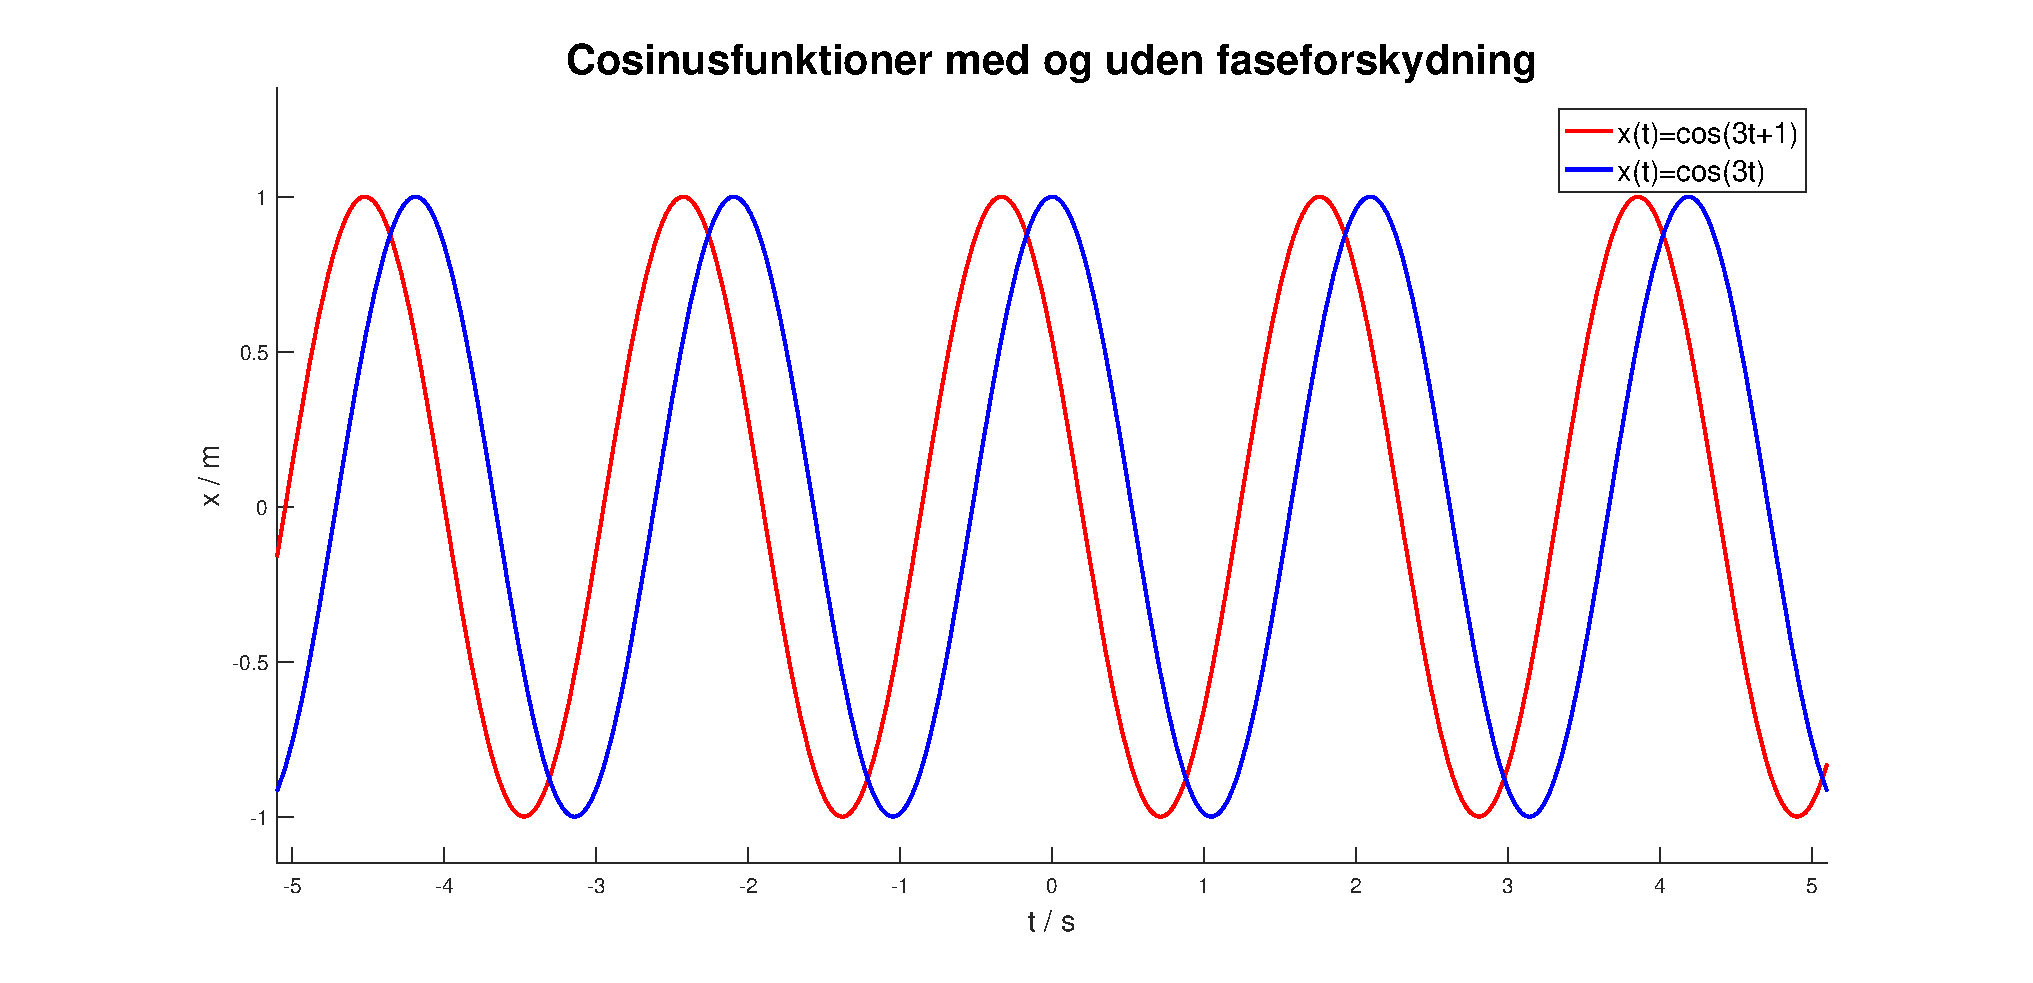
\includegraphics[width=.85\textwidth]{RotationelMekanik/Faseforskydning.eps}
\caption{Her ses to cosinusfunktioner, hvor den røde er faseforskydt i forhold til den blå med $\phi=1$. I fjedereksemplet svarer det til at tiden er startet, mens den blå er i $x=A$, og den røde er en smule foran.}
\label{fig:Faseforskydning}
\end{figure}
Det kan analogt til ligning \ref{eq:DiffLign} vises, at der tilføjes et additivt led, hvis en friktionskraft på formen $\v{f}=-b\v{v}$ medregnes
\begin{equation}
    \dd{x}{t} = -\frac{b}{m}\d{x}{t} - \frac{k}{m}x
\end{equation}
hvorved løsningen får tilføjet en eksponentiel faktor
\begin{equation}
x(t) = A\exp\left(-\frac{b}{2m}t\right)\cos\left(\omega' t + \phi\right), \qquad \omega' = \sqrt{\frac{k}{m}-\frac{b^2}{4m^2}}
\end{equation}
Harmonisk bevægelse kræver, at den resulterende kraft altid er rettet mod et hvilepunkt, der i fjederens tilfælde er loddets position i hvile. \\
For trigonometriske funktioner på følgende form
\begin{equation}
    f(x) = A\cos(B\cdot x + C)
\end{equation}
hvor $A,B,C$ er konstanter. $A$ er funktionens amplitude, og perioden er
\begin{equation}
    T = \frac{2\pi}{B}
\end{equation}
For roterende legemer kan ligning \ref{eq:N2R} bruges til at udlede bevægelsesligninger, hvor harmonisk bevægelse som det ovenstående kan forekomme nyttigt. Det kan være nyttigt at opskrive Newtons 2. lov for rotationel bevægelse på formen
\begin{equation}
    \dd{\theta}{t} = \alpha = \frac{1}{I}\sum\tau
\end{equation}
Vælges koordinatsystemet smart, kan problemet gøres mere overskueligt. Hvis der i den givne situation er en snorkraft eller normalkraft, hvis størrelse afhænger af de andre kræfter, kan origo placeres i den omtalte krafts angrebspunkt, hvorved kraftens arm og dermed kraftmomentet bliver nul. For $\v{r}_i=0$ er
\begin{equation}
    \gv{\tau}_i = \v{r}_i \times \v{F}_i = \v{0} \times \v{F}_i = \v{0}
\end{equation}
\chapter{Kerne- og Partikelfysik}
\section{Kernefysik}
I centrum af ethvert atom befinder sig en utrolig tæt, positivt ladet kerne. Atomets udstrækning er af størrelsesordenen $10^{-10}$ m, mens selve kernen kun udspænder cirka $10^{-15}$ m -- kernen er derfor 100.000 gange mindre end atomet. Alligevel befinder størstedelen af atomets masse sig i kernen. Atomkernen udgøres af postitive partikler \textit{protoner} (skrevet som ''p'') og neutrale partikler \textit{neutroner} (skrevet som ''n''). Kernen holdes sammen af den stærke kernekraft, én af de fire fundamentale kræfter. Denne kraft konkurrerer med den elektriske frastødning, som protonerne udøver på hinanden, og dette afgør, om kernen er stabil eller ustabil. Ustabile kerne kan henfalde - omdanne sig selv til en anden sammensætning ved en række processer. 
Dette afsnit vil give et kort overblik over kernefysikken - kategoriseringen af kernerne, hvilke modeller der kan bruges til at beskrive deres egenskaber og hvordan de kan gennemgå henfald. 

\subsection{Kernernes Egenskaber}
Eksperimentelt set har det vist sig, at atomets kerne kan ses som en kugle med radius $R$ indeholdene et antal \textit{nukleoner} - protoner og neutroner. Dette antal skrives som $A$. 
For de fleste kerner gælder det, at kernens radius kan udtrykkes som 
\begin{equation}
R = R_0A^{1/3},
\end{equation}
hvor $R_0$ er en eksperimentel konstant:
\begin{equation}
R_0 = 1,2\cdot {10^{-15}} ~ \SI{}{\m} = 1,2 ~\SI{}{\femto\m}. \footnotemark
\end{equation}

\footnotetext{ Her står ''fm'' for \emph{femto}-meter, hvor $\text{femto}=10^{-15}$}

\begin{table}
    \begin{tabular}{l|l|l|l}
    Partikel            & Masse, [kg]                      & Masse, [u]                       & Masse, [MeV/$\text{c}^2$] \\ \hline
    1 atomar masseenhed & 9,109 382 91 $\cdot 10^{-31}$   & 1                                & 931,494 061               \\
    Neutron             & 1,674 927 351 $\cdot 10^{-27} $ & 1,008 664 916 00                 & 939, 565 379              \\
    Proton              & 1,672 621 777 $\cdot 10^{-27}$  & 1,007 276 466 812                & 938, 272 046              \\
    Elektron            & 9,19 382 91 $\cdot 10^{-31}$    & 5,485 799 0946  $\cdot 10^{-4}$ & 0,510 998 928             \\
    \end{tabular}
    \caption{Massen af den atomare masseenhed, neutronen, protonen og elektronen i udvalgte enheder}
    \label{tab:masser}
\end{table}

Nukleon-tallet $A$ kaldes også for \emph{massetallet}, idet det lægger sig tæt op ad kernens masse udtrykt i \emph{atomare masseenheder}. Én atomar masseenhed, skrevet u eller $m_u$, er af historiske årsager defineret som en tolvtedel af massen af Carbon-12:

\begin{equation}
\text{u} = m_u \equiv \frac{1}{12} M(^{12}\text{C}).
\label{eq:u}
\end{equation} 

Tabel \ref{tab:masser} viser massen af den atomare masseenhed, samt neutronen, protonen og elektronen i enheder af henholdsvis kg, u og $\text{MeV}/\text{c}^2$ \footnotemark .

\footnotetext{Enheden $\text{MeV}/\text{c}^2$ er mega ($10^6$) elektronvolt over kvadratet af lysets hastighed $c$. Masse og energi er direkte koblet gennem Einsteins formel $E=mc^2$, ud fra det følger at en masse kan skrives som $m=E/c^2$.}

Det ses, hvordan protonens og neutronens masser er meget tæt på 1 u, og det er derfor $A$ tilnærmelsesvist giver massen af kernen i atomare masseenheder.

Som sagt er kernens massetal, $A$, antallet af nukleoner i kernen, altså summen af kernens antal protoner (skrevet som $Z$) og neutroner (skrevet som $N$):

\begin{equation}
A = Z + N.
\label{eq:A}
\end{equation}  

Kernens grundstof, også nogle gange kaldet kernens element, er bestemt af antal protoner, $Z$. For eksempel har hydrogen (H) altid én proton, helium (He) har to, og uran (U) har 92.
Kerner af det samme grundstof kan dog have forskellig masse ($A$) ved at have forskellige antal neutroner, $N$. Kerner med samme $Z$, men forskellig $N$ kaldes \emph{isotoper}. Tages uran ($Z=92$) som eksempel, er to almindeligt forekommende isotoper Uran--235 (massetal $A=235$ og $N=A-Z=143$) og Uran--238 ($N=146$). I fysikken kan vi bruge forskellig notation til at angive et grundstof på forskellige måder. Ser vi igen på Uran, kan vi angive hvilken isotop, der er tale om, ved at skrive "Uran--235", "U--235" eller 
\begin{equation*}
^{235}_{~92}\text{U}_{143}.
\end{equation*}

Her ses det, at notationen for et vilkårligt grundstof X følger:
\begin{equation*}
^{A}_{Z}\text{X}_{N},
\end{equation*}

men man vil oftest udelade informationen om $Z$ og $N$, idet grundstoffet selv er defineret ud fra $Z$, og $N$ opnås som $N=A-Z$. Man skriver derfor

\begin{equation}
^{A}\text{X}.
\end{equation}

\subsection{Kerners Binding}
I en kerne er nukleonerne samlet indenfor et begrænset område -- man siger, at kernen er et \emph{bundent system} \footnotemark .

\footnotetext{ En mere "fysisk" beskrivelse ville lyde på, at en partikel i et bundent system er udsat for et \emph{potential}, som kan holde partiklen lokaliseret. Potentialet kan være en ydre påvirkning (som et kraftfelt) eller kan være opstået som resultat af vekselvirkningen mellem det bundne systems komponenter. }

En vigtig egenskab for kernerne kan belyses gennem et simpelt eksempel. En alfa-partikel er et bundent system, bestående af to protoner og to neutroner (identisk til en helium--kerne). Massen af alfa-partikler i atomare masseenheder er målt til at være 4.001506179125 u. Den samlede masse af de to protoner og to neutroner kan udregnes til:

\begin{align*}
N \cdot m_n + Z \cdot m_p &= 2 \cdot 1,008 664 916 00~\SI{}{u} + 2 \cdot 1,007 276 466 812~\SI{}{u} \\
&= 4,031 88276562~\SI{}{u}.
\end{align*}  

Dette er ikke tilsvarende massen af alfa-partiklen! Faktisk ser vi, hvordan alfa-partiklen, det bundne system, har \emph{mindre} masse end summen af masserne for de tilstedeværende protoner og neutroner! Dette er tilfældet for alle kerners masse sammenlignet med massen af de individuelle nukleoner. Dette skyldes, at det bunde system har mindre \emph{potentiel energi}, end hvad de individuelle nukleoner oplever. Simpelt sagt kan man sige, at noget af massen "forsvinder" og bliver lagret i form af energi, når individuelle nukleoner bliver bundet sammen i kerner.

Forskellen i masse mellem kernen og massesummen af nukleonerne kaldes for \emph{massedefekten}, skrevet som $\Delta M$ (udtales "delta-M"):

\begin{equation}
\Delta M \equiv M(Z,A) - Z (m_p + m_e) - N \cdot m_n.
\label{eq:mass_excess}
\end{equation}

Læg mærke til, at massen $m_e$ -- elektronens masse -- optræder i formlen. Dette skyldes at $M(Z,A)$ er den \emph{atomare masse} af elementet, massen af kernen medtaget elektronerne om kernen. Et "uændret" atom er neutralt, og har derfor lige mange protoner og elektroner, derfor ganges $m_e$ med antallet af protoner $Z$.
 
Vi kan vende tilbage til vores eksempel med alfa-partiklen og udregne massedefekten. I dette tilfælde har vi massen $M_\alpha$ af alfa-partiklen opgivet ($M(2,4)$, uden bidraget fra elektronerne), svarende til størrelsen $M_\alpha=M(2,4)-2\times m_e$. Massedefekten udregnes da som:

\begin{align*}
\Delta M &= M_\alpha + 2\cdot m_e - Z(m_p + m_e) - N \cdot m_n \\
&= M_\alpha - Z \cdot m_p - N \cdot m_n \\
&= 4,001506179125~\SI{}{u} - 2 \cdot 1,008 664 916 00~\SI{}{u} - 2 \cdot 1,007 276 466 812~\SI{}{u} \\
&= -0,03037658649~\SI{}{u}
\end{align*}

Dette er altså forskellen mellem massen af alfa-partiklen og massen af de to protoner og to neutroner. Masse og energi er ækvivalente gennem Einsteins formel

\begin{equation}
E = m c^2, 
\label{eq:einstein}
\end{equation}

hvor $c$ er lysets hastighed.
Så hvad svarer den manglende masse til i energi? Læg her mærke til, at den atomare masseenhed u også kan udtrykkes i den meget praktiske enhed $\text{MeV}/c^2$, hvor $1~\SI{}{u}=931,494061~\SI{}{MeV}/c^2$. Derfor kan vi direkte omregne massedefekten til energi:

\begin{align*}
E &= \Delta M c^2 \cdot 931,494061~\SI{}{MeV}/c^2/\SI{}{u} \\
&= -0,03037658649 ~\SI{}{u} c^2 \cdot 931,494061~\SI{}{MeV}/c^2/\SI{}{u} \\
&= -28,2956099089 ~\SI{}{MeV}
\end{align*}

Denne størrelse -- uden fortegnet! -- er kernens \emph{bindingsenergi}. Bindingsenergien er den energi, som skal tilføres det bundne system for at skille det ad til dets individuelle nukleoner. Jo større bindingsenergi, desto sværere er det at skille kernen ad, sagt med andre ord, at jo højere bindingsenergi, desto mere stabil er kernen. Omvendt er bindingsenergien den energi der udløses, ved at samle frie nukleoner --  eller kerner -- til større systemer. Dette er princippet bag \emph{fusion}, den sammensmeltning af mindre elementer til tungere elementer, som foregår i Solen og andre stjerner for at producere energi.
Bindingsenergi, skrevet $E_B$ udtrykkes altid som en positiv størrelse. Udtrykt som funktion af massedefekten kan vi derfor skrive:
\begin{equation}
E_B = - \Delta M c^2.
\label{eq:binding}
\end{equation} 

En kernes bindingsenergi vil ændre sig, hvis der tilføjes eller fjernes nukleoner fra kernen, og \emph{vil altid stige med antallet af nukleoner, $A$}. Selvom nukleonerne i sig selv ikke besidder bindingsenergi, kan vi forestille os, at bindingsenergien for en kerne kan deles ligeligt mellem dens nukleoner. Denne størrelse kaldes for (den gennemsnitlige) bindingsenergi per nukleon, $E_B/A$. Figur \ref{fig:binding} viser $E_B/A$ som funktion af $A$. 

\begin{figure}[h]!
  \centering
  \includegraphics[width=0.6\textwidth]{KernePartikel/binding_energy.png}
  \caption{Bindingsenergi per nukleon som funktion af massetallet, $A$}
  \label{fig:binding}
\end{figure}

Figuren angiver udvalgte kerner, for eksempel He-3 ($Z=2,N=1$), He-4($Z=2,N=2$) og Fe-56 (jern-56, $Z=26,N=30$). Vi kan gøre os følgende observationer; først og fremmest vokser $E_B/A$ stejlt for de lette kerner. Kurven ser ud til at toppe omkring Jern--56. Herefter falder bindingsenergien per nukleon langsomt igen for de tunge kerner. Desuden er kurven heller ikke "glat",  men viser udslag af høje bindingsenergier for bestemte kerner, He--4, Ca--12 (Carbon--12), O--16 (Oxygen--16)... Vi skal senere vende tilbage til, hvorfor netop kernerne  He-4, Ca-12, og O-16 udviser høj bindingsenergi, altså er særlig stabile.

\subsection{Stabile og Ustabile Kerner}
Kerner kan enten være stabile eller ustabile. At en kerne er stabil betyder, at den, ulig de ustabile kerner, ikke er radioaktiv, det vil sige, at den ikke spontant undergår radioaktiv henfald. Når der snakkes om stabile kerner, mener man stabile isotoper, idet det samme element både kan have stabile og ustabile isotoper. Vi kan prøve at plotte de eksperimentelt bestemte stabile isotoper ud fra deres værdier af $Z$ og $N$. Et sådan plot er vist i Figur \ref{fig:stable_iso}.

\begin{figure}[h!]
  \centering
  \includegraphics[width=0.6\textwidth]{KernePartikel/stable_nucleides.jpg}
  \caption{Stabile isotoper (markeret som sorte firkanter) og deres værdier af $Z$ og $N$.}
  \label{fig:stable_iso}
\end{figure}

Indtegnet på figuren er også linjen svarende til $Z=N$. Det ses, hvordan de lette kerner (små værdier af $Z$ og $N$) ligger op ad denne linje, men efterhånden som vi bevæger os mod de tungere kerner (højere værdier af $Z$ og $N$), afviges der fra den rette linje, og isotoper med højere $N$ favoriseres over isotoper med højere $Z$. Den snævre region af stabile kerner vist i Figur \ref{fig:stable_iso} kaldes for \emph{stabilitetslinjen} \\
Plottet vist i Figur \ref{fig:known_iso} viser alle kendte isotoper, med de stabile isotoper igen markeret i sort. Det ses, hvordan kerner ikke er fundet til at have vilkårlige antal $Z$ og $N$, eksempelvis ses ingen kerner til at have $Z=50, N=20$ eller $Z=100, N=100$. Generelt er der ingen kerner som udviser meget stor forskel mellem $Z$ og $N$, meget højt protonantal ($Z \gtrsim 80$) eller er ekstremt tunge ($A \gtrsim 200$). 

\begin{figure}[h!]
  \centering
  \includegraphics[width=0.6\textwidth]{KernePartikel/known_nucleides.jpg}
  \caption{ Alle kendte isotoper ud fra deres værdier af $Z$ og $N$. Stabile isotoper er markeret som sorte firkanter, mens ustabile isotoper er markeret med lysegrå firkanter}
  \label{fig:known_iso}
\end{figure}


Vi vil komme til at se, at ustabile kerner kan "vinde"  energi ved at undergå radioaktivt henfald og ændre komposition, således at de bevæger sig tættere på stabilitetslinjen i $NZ$-plottet. Eksempelvis vil kerner, som har mange neutroner i forhold til protoner (kernerne, som ligger under stabilitetslinjen) spontant omdanne en af deres neutroner til en proton i det der hedder et $\beta^-$-henfald, mens meget tunge kerner kan brydes op i to mindre kerner, hvoraf én typisk er $^4\text{He}$.  

\subsection{Magiske Tal og Skalmodellen}

Vi skal nu vende de særligt stabile kerner, som viser sig i Figur \ref{fig:binding} ved at have særlig høj $E_B/A$. Denne opførsel kan forudsiges ved at beskrive kernen ud fra et bestemt billede, kaldet skalmodellen, og med denne kan vi forstå, hvorfor eksempelvis $^4\text{He}$ er så stabil.
Skalmodellen minder i princippet om et andet fænomen, I nok har hørt om i forbindelse med elektronskaller. Elektroner bundet i et atom kan ses som at arrangere sig i bestemte "baner" eller skaller om atomkernen. Hver skal kan holde et bestemt antal elektroner, og elektronerne vil generelt fylde skallerne nedefra og op. Atomer, hvis elektronskaller alle er fyldt op, deltager ikke i kemiske reaktioner. Dette kender vi fra ædelgasserne.
Tilbage til skalmodellen og kerne--billedet. Selvom billedet er mere komplekst, så kan kernen på samme måde som atomet siges at bestå af en række skaller og underskaller. Men i stedet for at fylde skallerne op med elektroner, skal skallerne fyldes med protoner og neutroner. Grundet Paulis udelukkelsesprincip, kan der kun eksistere et endeligt antal protoner eller neutroner i en skal. Bestemte antal af $Z$ og $N$ vil på samme måde som elektronerne, svare til fyldte skaller. Ud fra skalmodellen er disse forudset til at være

\begin{equation}
2,8,20,28,50,82,126, ~\text{magiske tal for $Z$ og $N$}.
\label{eq:magicnumbers}
\end{equation}

Disse kaldes for \emph{magiske tal}. Det er altså for disse proton- og neutron-antal, at bindingsenergien per nukleon er usædvanlig høj. Bemærk at selvom $Z=126$ er forudsagt som en "magisk"  kerne, så er denne kerne ikke observeret i naturen. Det er også muligt for en kerne at være dobbelt-magisk, i så fald er både $Z$ og $N$ magiske tal. Dette gælder blandt andet for kernerne

\begin{equation*}
^{4}_{2}\text{He},~~ ^{16}_{~8}\text{O},~~ ^{40}_{20}\text{Ca},~~ ^{48}_{20}\text{Ca},~~  ^{208}_{82}\text{Pb}. 
\end{equation*}

\subsection{Kerners Henfald}

Omkring 90\% af alle kendte kerner er radioaktive og kan derfor henfalde spontant. Som nævnt i det foregående afsnit, vil et henfald af en ustabil kerne bringe kernen tættere på stabilitetslinjen i $NZ$-kortet. For et henfald som ændrer kompositionen af kernen (ændrer $Z$ eller $N$) benævnes den originale kerne som \emph{moder-kernen}, mens slutproduktet kaldes for \emph{datter-kernen}. Et henfald kan foregå spontant (naturligt) såfremt massen af det originale atom (tit kaldet den initiale masse, $M_i$) er større end massen af slutproduktet (den finale masse, $M_f$). I enheder af energi er forskellen mellem de to simpelt skrevet som:

\begin{equation}
Q =(M_i - M_f)c^2.
\label{eq:Qvalue}
\end{equation}

Dette tal kaldes for reaktionens $Q$-værdi. Det ses, at for reaktioner med positiv $Q$-værdi (såkaldt exo-energiske reaktioner) må det gælde at $M_i > M_f$, og det er altså disse reaktioner, som kan foregå. Nedenfor gennemgås nogle almindelige slags henfald; alfa-- og beta--henfald, som ændrer kompositionen af kernerne, og gamma--henfald, som er et indre henfald af et anslået atom, og derfor ikke ændrer $Z$ eller $N$.

\subsubsection{Alfa-henfald}
Et alfa-henfald sker når moderkernen udskiller en alfa-partikel. Skematisk kan vi skrive:
\begin{equation}
\text{alfa--henfald}: ^A_Z\text{X} \rightarrow ^{A-4}_{Z-2}\text{Y} + ^4_2\text{He}.
\label{eq:alfa} 
\end{equation}

Normalt skelner man mellem notationen $\alpha$ (helium--kerne) og $^4_2\text{He}$ (helium--atom). Ved at skrive $^4_2\text{He}$ i reaktionsskemaet angiver man, at der regnes med atomare masser, og ikke kernemasser -- på denne måde er ladningen også bevaret i reaktionen. Anvend derfor den atomare masse af $^4_2\text{He}$ medmindre andet er angivet.

\subsubsection{Beta-henfald}
Der findes tre former for beta-henfald, kaldet beta--minus (skrevet som $\beta^-$), beta-plus ($\beta^+$) og elektronindfangning. Ligesom ved alfa--henfaldet er henfaldet navngivet efter den partikel, der udsendes i reaktionen. En beta--minus--partikel er en elektron. Det er ikke åbenlyst hvordan en kerne kan udsende en elektron, når den kun består af neutroner og protoner, men vi ser, hvordan henfaldet omhandler omdannelsen af en neutron til en proton. Dette slags henfald forekommer derfor for kerner, som har mange neutroner i forhold til protoner (kerner som befinder sig under stabilitetslinjen i $NZ$-plottet vist i Figur \ref{fig:known_iso}). Omdannelsesprocessen forløber således:
\begin{equation}
\text{$\beta^-$-henfald: }n \rightarrow p + e^- + \bar{\nu}_e
\end{equation}
eller skrevet ved brug af kerne-notation:

\begin{equation}
\text{$\beta^-$-henfald: } ^A_Z\text{X} \rightarrow ^A_{Z+1}\text{Y} + e^- + \bar{\nu}_e
\end{equation}

Partiklen angivet som $\bar{\nu}_e$ er en \emph{anti--neutrino} (hvor en neutrino skrives som $\nu_e$ ved det græske bogstav "nu"). Vi skal i kapitlet om partikelfysik gennemgå nogle simple love, der dikterer, hvorfor henfaldet kræver udsendelse af en anti-neutrino, men for nu bliver vi nødt til bare at godtage dens tilstedeværelse. Neutrinoen og anti--neutrinoen er effektivt masseløse, så der skal ikke tages højde for dem under beregning af $Q$--værdi. 

$\beta^+$--henfald forekommer for kerner, som har mange protoner i forhold til neutroner. Her udsendes elektronens anti--partikel, \emph{positronen} ($e^+$), og en neutrino:

\begin{equation}
\text{$\beta^+$--henfald: } p \rightarrow n + e^+ + \nu_e,
\end{equation} 

 som ved brug af kerne--notation skrives som
 
\begin{equation}
\text{$\beta^+$--henfald: } ^A_Z\text{X} \rightarrow ^A_{Z-1}\text{Y} + e^+ + \nu_e.
\end{equation}

Den sidste form for beta--henfald kaldes for elektronindfangning (\emph{eng: electron capture}, forkortet EC). Dette er en proces, hvor kernen "fanger" en af atomets inderste elektroner og omdanner den til en neutron:

\begin{equation}
\text{EC: } p + e^- \rightarrow n + \nu_e,
\end{equation}

som skrives som:

\begin{equation}
\text{EC: } ^A_Z\text{X}~\rightarrow~^A_{Z-1}\text{Y} + \nu_e.
\end{equation}

\subsubsection{Gamma-henfald}
Kerner, som gennemgår et henfald eller en kollision, kan ende i en anslået (exciteret) tilstand. Dette betyder, at kernens nukleoner ikke befinder sig i den lavest mulige energitilstand (kaldet grundtilstanden), men besidder "ekstra" energi i kraft af at befinde sig i en højere energitilstand. For at "falde tilbage"  til grundtilstanden skal kernen give afkald på den ekstra energi, og dette sker under udsendelse af en \emph{foton}, skrevet med symbolet $\gamma$ (det græske bogstav "gamma"). Denne slags henfald kaldes for et gamma-henfald. En foton, også kaldet en lys--kvant, besidder en energi, men ingen ladning. Et gamma-henfald kan derfor ikke ændre på sammensætningen af en kerne, og $A,Z$ og $N$ ændres derfor ikke. En kerne, som er exciteret angives normalt med symbolet " * ". Et gamma--henfald kan derfor skrives skematisk som

\begin{equation}
\text{gamma-henfald: } ^A_Z\text{X}^* \rightarrow ^A_Z\text{X} + \gamma.
\end{equation}
\newpage

\section{Partikelfysik}
\label{cha:partikel}

Partikelfysik er den gren af fysikken, som beskæftiger sig med
universets mindste bestanddele og deres vekselvirkning med hinanden.
Vi har indtil videre stiftet bekendtskab med en del allerede;
elektronen, protonen, neutronen og neutrinoen, og du har måske selv
hørt om partikler som muonen og Higgs--bosonen. Partikelfysikkens
zoologiske have indeholder en bred vifte af partikler, hvoraf de mest
fundamentale partikler er elementarpartiklerne -- partikler, som man
mener ikke kan deles. Heriblandt er elektronen, neutrinoen og
kvarkerne. Kvarker i sammensætning udgør hadronerne, som protonerne og
neutronerne er eksempler på. Dette afsnit vil give et kort overblik
over partiklerne, deres egenskaber og fysikkens indtil videre bedste
bud på et samlet billede af alt i verden, kaldet standardmodellen.

\subsection{Standardmodellen}
Standardmodellen er teorien om de elementare partikler og hvordan de
fire fundamentale naturkræfter -- tyngdekraften, den elektromagnetiske
kraft og den stærke og svage kernekraft -- vekselvirker.

\subsubsection{Partikler og anti-partikler}
Der arbejdes her med tre egenskaber for partiklerne: masse, ladning og
\emph{spin}. Spin er en kvantemekanisk egenskab for en partikel, som
ikke har nogen analog i den makroskopiske fysiske verden\footnotemark,
men det besidder altid en bestemt størrelse og en retning, og er
vigtigt, hvis man vil regne kvantemekanisk på partiklerne.
\footnotetext{Nogle bøger i gymnasiet beskriver en partikels spin, som
  at man kan forestille sig, at partiklen drejer om sig selv på samme
  måde som at Jorden roterer, men dette billede er fundamentalt
  forkert og skal slettes fra din bevidsthed så hurtigt som muligt.}
Alle partikler har en \emph{antipartikel}. En antipartikel er ens i
alle henseender med sin partikel bortset fra sin ladning (og andre
tekniske egenskaber, som vi ikke vil komme ind på her). Den negativt
ladede elektron, $e^-$, har antipartiklen kaldet positronen (også
nogle gange kaldet anti-elektronen), $e^+$. De to partikler har samme
masse og spin, men modsatte ladninger. Hvis en elektronen og en
positron ''møder'' hinanden, ophæver de hinanden og de eksisterer ikke
længere. Dette kaldes for en \emph{annihilation}. På grund af energi--
og impulsbevarelse, bliver der i en annihilation altid skabt partikler
til at bære den overskydende energi væk. En annihilation mellem en fri
elektron og en positron skaber to fotoner:
\begin{equation}
e^- + e^+ \rightarrow \gamma + \gamma 
\end{equation}
Fotonerne har ingen masse, men får sin energi fra masserne af
elektronen og positronen gennem Einsteins formel $E=mc^2$, der giver
en ækvivalens mellem energi $E$ og masse $m$, idet $c$ blot er en
naturkonstant (lysets fart i vakuum). For visse partikler gælder det,
at de er sin egen antipartikel, fx fotonen. To fotoner kan eksempelvis
annihilere i den omvendte reaktion:
\begin{equation}
\gamma + \gamma \rightarrow e^- + e^+,
\end{equation}
så længe reaktionen overholder energi-- og impulsbevarelse.

Standardmodellens elementare partikler er vist skematisk i Figur
\ref{fig:standard}. De er leptonerne, kvarkerne (eng: \emph{quarks}),
de vekselvirkende eller kraftbærende partikler (kaldet
\emph{gauge-bosoner}) og Higgs-bosonen.
\begin{figure}[h!]
  \centering
  \includegraphics[width=0.6\textwidth]{KernePartikel/fig_p/standard.png}
  \caption{ Standardmodellens elementarpartikler: leptonerne,
      kvarkerne, gauge-bosonerne og Higgs-bosonen. Til venstre i hver
      kasse ses partiklens masse, ladning og spin.}
  \label{fig:standard}
\end{figure}

\subsubsection{Leptoner}
Leptonerne er en gruppe af elementare partikler, som ikke vekselvirker
gennem den stærke kernekraft. Alle leptoner har spin $s = 1/2$, og er
derfor det, der kaldes \emph{fermioner}.

Leptonerne er overordnet delt ind i tre grupper, kaldet
generationer. Én generation af leptoner består af en ladet partikel og
en neutral partikel. Vi har allerede stiftet bekendtskab med én
generation af leptoner, nemlig den ladede elektron, $e^-$ og den
neutrale (elektron)neutrino, $\nu_e$. Næste generation af leptoner
udgøres af \emph{muonen} (skrevet som det græske bogstav 'mu', $\mu$)
og muon--neutrionen, $\nu_\mu$. Sidste generation af leptoner er den
tunge partikel \emph{tau} (skrevet som det græske bogstav, 'tau',
$\tau$) og tau--neutrinoen, $\nu_\tau$ . Muonen og tau--partiklen, der er
meget massive i forhold til elektronen, er ustabile og vil derfor
hurtigt henfalde til elektroner. De kan på grund af deres høje masser
kun dannes i høj--energi kollisioner, som dem der foregår i
partikelacceleratorer eller reaktioner involverende kosmisk stråling
(husk, at masser og energi er det samme i partikelfysikken, så det
kræver meget energi at skabe tunge partikler).

Leptonerne, inklusiv antipartiklerne $e^+,\bar{\mu}, \bar{\tau},
\bar{\nu}_e...$ kan påvirkes af tyngdekraften, den elektromagnetiske
kraft og den svage vekselvirkning.

\subsubsection{Kvarkerne}
Kvarkerne er de partikler som kan sammensættes til blandt andet
protonerne og neutronerne. En speciel egenskab for kvarkerne gør, at
de aldrig kan findes isoleret, og kvarkerne kan derfor aldrig
observeres direkte. De er spin 1/2-partikler ligesom leptonerne, og
besidder forskellige brøkdele af elementarladningen, som det ses af
Figur \ref{fig:standard}.

De er navngivet up, down, charm, strange, top og bottom med symbolerne
u, d, c, s, t og b. En vilkårlig kvark angives som q, og en antikvark
som $\bar{\text{q}}$. Kvarkernes egenskaber og evidens for deres
eksistens er opdaget ved at studere hadroner (altså de partikler, som
kvarkerne er byggesten for, se afsnit \ref{sec:hadron}), og de første
kvarker blev studeret i slutningen af 1960'erne, mens den sidste og
tungeste kvark, top--kvarken, blev opdaget i 1995.

Kvarkerne er de eneste partikler som kan vekselvirke gennem alle fire
fundamentale kræfter.

\subsection{De Fundamentale Kræfter og Gauge--bosoner}
Standardmodellen arbejder med fire fundamentale kræfter. Tabel
\ref{tab:forces} viser de fire former for vekselvirkning, og deres
styrke relativ til den stærkeste kraft, den stærke vekselvirkning.

\begin{table}[h]
\centering
    \begin{tabular}{l|l|l|l}
    Vekselvirking    & Relativ styrke  & Rækkevidde                   & Partikel                   \\ \hline
    Stærk            & 1               & kort ($\sim \SI{1}{fm}$)     & gluon, g                   \\
    Elektromagnetisk & $\frac{1}{137}$ & lang ($1/r^2$)               & foton, $\gamma$            \\
    Svag             & $\sim 10^{-9}$  & kort  ($\sim \SI{0.001}{fm}$) & $\text{W}^\pm, \text{Z}^0$ \\
    Gravitationel    & $\sim 10^{-38}$ & lang ($1/r^2$)               & graviton                   \\
    \end{tabular}
    \caption{De fire fundamentale kræfter og deres
        vekselvirkningspartikler, hvoraf gravitonen endnu ikke er
        eksperimentelt bekræftet.}
    \label{tab:forces}
\end{table}

Den elektromagnetiske vekselvirkning og tyngdekraften kendes fra
klassisk fysik, som kræfter, hvis styrke afhænger af afstanden mellem
de vekselvirkende objekter som $1/r^2$. Den stærke vekselvirkning, er
ansvarlig for den stærke kernekraft, som holder nukleonerne i kernen
sammen. Den har en kort rækkevidde, typisk omkring udstrækningen af en
kerne. I følgende afsnit skal vi lære, at kvarkerne vekselvirker med
hinanden ved hjælp af den stærke vekselvirking. Den svage
vekselvirkning er ansvarlig for beta--henfald, og henfaldet af ustabile
partikler såsom leptonerne.

Standardmodellen beskriver vekselvirkninger gennem de fundamentale
kræfter som udvekslingen af en partikel kaldet en
gauge-boson. Forestil dig to elektroner, som er på vej til at
mødes. De vil frastøde hinanden på grund af deres ladning, men hvordan
ved elektronerne at den anden elektron er til stede? Det ved de fordi
der sker en udveksling af en gauge-boson, i dette tilfælde fotonen.

I dette billede ''bærer'' eksempelvis fotonen den elektromagnetiske
vekselvirkning. Det betyder, at to partikler som interagerer
elektromagnetisk, vil udveksle en foton. De andre gauge-bosoner er
\emph{gluonen}, g, som bærer den stærke vekselvirning og W-- og
Z--partiklerne, som udveksles i reaktioner involverende den svage
kernekraft. Modsat gluonen og fotonen, har Z-- og W--bosonerne masse
(man siger, at de er massive). Z--bosonen er uden ladning, mens
W--bosonen enten kan have positiv eller negativ ladning skrevet
henholdsvis som $\text{W}^+$ og $\text{W}^-$.

Når en gauge--boson udveksles mellem to partikler -- altså når to
partikler vekselvirker gennem en fundamental kraft -- siger man, at
partiklen er \emph{virtuel}. At en partikel er virtuel betyder, at den
''matematisk'' er til stede, men ikke fysisk kan observeres.  Gauge-bosoner har altid et heltalligt
spin, $s = 0,1,2,\dots$

Standardmodellen er en uhyre god fysisk teori, og har gang på gang
vist sig at give korrekte forudsigelser om forskellige
eksperimenter. Desværre har den ét stort problem: Teorien indeholder
ikke tyngdekraften, så standardmodellen indeholder faktisk kun tre ud
af de fire fundamentale naturkræfter. Man kan fikse problemet ved at
tilføje en hypotetisk graviton--partikel, der skulle bære den
gravitationelle vekselvirkning. En komplet fysisk teori må
naturligvis indeholde alle fire naturkræfter, og indtil videre er der
ingen troværdig fysisk teori, der formår dette. Der findes dog
eksotiske bud på sådanne komplette teorier, såsom strengteori og
supersymmetri, men disse har andre store problemer, så der kun er få
fysikere, der tror på dem.

\subsubsection{Higgs--bosonen}
Higgs--bosonen er en partikel, hvis eksistens var forudsagt inden den
blev opdaget i 2013. Higgs--partiklen skaber et felt kaldes
Higgs-feltet, fra hvilket massive partikler får deres masse
fra. Higgs--feltet var en af mange teorier omkring, hvordan masse
skabes, og kan forklare, hvorfor Z og $\text{W}^\pm$ har masse,
hvilket ellers ikke umiddelbart var forventet for
gauge--bosoner. Higgs--partiklen er meget tung, og kræver derfor stor
energi for at kunne skabes i partikelacceleratorer. Derfor er det også
først for nyligt, at man kunne producere partiklen. Efter sin dannelse
vil den meget hurtigt henfalde til lettere partikler.

\subsection{Kvarker i Sammensætning -- Hadroner}
\label{sec:hadron}
Vi lærte i forrige afsnit, at kvarker ikke kan eksistere i
isolation. Kvarker bindes i stedet sammen via den stærke kernekraft i
systemer og danner sammensatte partikler. De sammensatte partikler
(eng: \emph{composite particles}) kaldes samlet set for
\emph{hadroner}.  Der eksisterer to typer hadroner: baryonerne og
mesonerne. Baryonerne er sammensatte partikler bestående af tre
kvarker, mens mesonerne består af et kvark--antikvark--par. Dette er
illustreret i Figur \ref{fig:baryonmeson}.
\begin{figure}[htb]
  \centering
  \includegraphics[width=0.3\textwidth]{KernePartikel/fig_p/baryonmeson.png}
  \caption{ Baryoner består af tre kvarker, mens mesoner
      består af en kvark og en antikvark, f.eks. pionen, $\pi^+$, hvis
      kvarkindhold er én u-kvark og én anti-d-kvark, eller
      b-eta-mesonen, $\eta_b$, hvis kvark indhold er én b-kvark og én
      anti-b-kvark.}
    \label{fig:baryonmeson}
\end{figure}
Protoner og neutroner er eksempler på baryoner. Deres sammensætning er
vist i Figur \ref{fig:protonneutron}.
\begin{figure}[htb]
  \centering
  \includegraphics[width=0.3\textwidth]{KernePartikel/fig_p/composite.png}
  \caption{ Protonen og neutronen består af hver tre
      kvarker. Deres antipartikler består af antikvarkerne.}
  \label{fig:protonneutron}
\end{figure}
En proton består af to u--kvarker og én d--kvark, mens neutronen består
af to d--kvarker og én u--kvark. Vi kan forstå mange af deres egenskaber
ved at se på deres kvarksammensætning. Den samlede ladning af
kvarkerne i protonen kombineres til $1$ elementarladning, mens
kvarkerne i neutronen kombineres til ladning 0. Da forskere fandt ud
af, at neutronen besad en magnetisk egenskab kaldet et \emph{magnetisk
  moment}, var det en gåde for dem, hvordan det kunne lade sig gøre
for en neutral partikel, men nu ser vi, hvordan dette skyldes de
magnetiske egenskaber for neutronens individuelle kvarker, som jo
netop har ladning. Vi ser også, hvordan masserne af protonen og
neutronen (omkring \SI{930}{MeV/c^2}) er meget større end massen af de
individuelle up- og down-kvarker, der hver kun vejer \SI{2,3}{MeV/c^2}
og \SI{4,8}{MeV/c^2}), hvor den manglende masse kommer fra
gluonfeltet, som binder kvarkerne sammen. Baryonernes og mesonernes
antipartikler består simpelt af antikvarkerne i stedet for for kvarker
(vist i Figur \ref{fig:protonneutron}).

\subsection{Partikelreaktioner}
Under udarbejdelsen af standardmodellen, så man, hvordan visse
vekselvirkninger og henfald skete ofte, mens andre fandt sted med
langt mindre sandsynlighed eller slet ikke -- såkaldte \emph{forbudte}
reaktioner. Studiet af de forekommende reaktioner har ledt til en
række bevarelseslove, som dikterer hvilke reaktioner, som kan
forekomme, og hvilke der ikke kan. Der skal vanskeligt matematik til
for at regne på reaktionerne, men de kan simpelt visualiseres ved
brugen af såkaldte Feynman-diagrammer.
 
\subsection{Bevarelseslove}
I fysikken dikterer en bevarelseslov at en størrelse ikke ændrer sig
over tid. De fleste har allerede stiftet bekendtskab med koncepter som
energi--, impuls-- og ladningsbevarelse, som også dikterer interaktioner
mellem partikler. Ud over disse bevarelseslove er to andre størrelser
i partikelfysikken bevarede, nemlig \emph{baryon--tal} og
\emph{lepton--tal}. Disse tal kan ses lidt ligesom bevarelsen af den
samlede ladning i en reaktion. Idéen er, at alle baryoner besidder
baryontallet $B=1$, mens deres antipartikler besidder
$B=-1$. Alternativt kan man sige at kvarker har $B=1/3$, mens
antikvarker har $B=-1/3$. Alle partikler som ikke er dannet af kvarker
har automatisk $B=0$. Et eksempel kan være reaktionen:
\begin{equation*}
p + n \not\rightarrow p + \mu^+ + \mu^- .
\end{equation*}
Ladningen er bevaret i denne reaktion, men baryon--tallet er ikke
bevaret, idet vi på højresiden har $B=1+1$, mens vi på venstresiden
har $B=1$, da muonerne begge har $B=0$. Reaktionen vil altså ikke
forekomme!

Lepton-tallet fungerer på samme måde. Her har alle medlemmmer af
lepton--familien ($e^-,\nu_e, \mu^-$, \dots) lepton--tal $L=1$, mens
deres antipartikler ($e^+, \bar{\nu}_e, \mu^+$, \dots) har $L=-1$. Man
skelner også mellem lepton--tal for de forskellige generationer,
skrevet $L_e, L_\mu,L_\tau$ for henholdsvis elektronen, muonen og
tau--partiklen og deres neutrinoer. Disse skal også være bevaret
individuelt.\footnote{Dette er faktisk en sandhed med modifikationer,
  fordi bevarelsen af de enkelte generationers leptontal kan brydes i
  visse tilfælde, men det er meget usandsynligt, så vi vil antage, at
  de altid er bevarede.} Et eksempel er henfaldet af en neutron:
\begin{equation*}
n \rightarrow \bar{p} + e^- + \bar{\nu_e}.
\end{equation*} 
Neutrinoer interagerer så lidt med stof, at de er meget svære at
detektere. Derfor kunne man, baseret på observationer, fristes til at
tro, at reaktionen forløb som $n \rightarrow \bar{p} + e^-$, men dette
passer ikke med den energi, som anti--protonen og elektronen besidder
efter et sådant henfald. Der må være en tredje partikel til
stede. Anti--neutrinoens tilstedeværelse bevarer både energi og
lepton--tal i henfaldet af en neutron.

\subsection{Feynman--Diagrammer}
\label{sec:feyman}
Feynman--diagrammer, udviklet af den berømte amerikanske fysiker
Richard Feynman (1918-1988), er visuelle repræsentationer af
vekselvirkningen mellem partikler. Deres enkelhed gør dem til et
must-have i alle partikelfysikeres værktøjskasse, og de kan anvendes
og forstås uden kompliceret matematik. Dette afsnit gennemgår først
fremgangsmåden for at konstruere et feynman-diagram, og dernæst den
underlæggende fysiske betydning. Reglerne er meget simple!

\subsubsection{Basis konstruktion af feynman-diagrammer}

\begin{enumerate}

\item Først og fremmest arbejdes der med to slags symboler: den lige
  linje med en pil og den bugtede linje:
	\begin{minipage}[c]{\textwidth}
	\centering
     \includegraphics[width=6 cm]{KernePartikel/fig_p/symbols.png}
	\end{minipage}
Pilen kan både pege den ene og den anden vej!

\item De to slags linjer kan forbindes, men kun hvis to linjer med
  pile forbindes med en enkelt bugtet linje. Således:
	\begin{minipage}[c]{\textwidth}
	\centering
     \includegraphics[width=5 cm]{KernePartikel/fig_p/QEDvertex2.png}
	\end{minipage}
        Det punkt, som kombinerer de tre linjer kaldes for et
        \emph{vertex}. Læg mærke til retningen for pilene! Det skal
        gøres således, at \emph{ hver gang en pil peger mod et vertex,
          skal der være en pil, som peger væk fra vertexet}.
\end{enumerate}
Hvad betyder det, fysisk set?  Hver linje i regel (1) er en
partikel. Linjerne med pile er fermioner (elektroner, kvarker, osv.),
mens den bugtede linje kan repræsentere en boson (fotonen, gluonen,
osv.). Dog anvender man normalt forskellige symboler for de
forskellige slags vekselvirkninger, mere om det i opgaveafsnittet.
Vertexet (knudepunktet) er en vekselvirkning/interaktion. Virtuelle partikler eksisterer mellem to vertexer. 

Diagrammerne fortæller en historie om partiklernes vekselvirkning. Vi læser dem fra
venstre mod højre,som det er illustreret i Figur \ref{fig:axis}.
\begin{figure}[h!]
  \centering
  \includegraphics[width=0.3\textwidth]{KernePartikel/fig_p/axis2.png}
  \caption{ Feynman-diagrammer har tiden ad $x$-aksen.}
  \label{fig:axis}
\end{figure}
Normalt tegner man ikke aksen på, som det er gjort i Figur
\ref{fig:axis}, men det kan for nogle være en hjælp, så gør hvad du
føler dig tryg ved. At det er vigtigt at være opmærksom på, at
feynman--diagrammer læses fra venstre mod højre kan illustreres i et
eksempel. Vi kigger her på vekselvirkningen involverende tre
partikler: en elektron, positron og en foton.
\begin{figure}[h!]
  \centering
  \includegraphics[width=8 cm]{KernePartikel/fig_p/elektron_positron2.png}
  \caption{Elektronen, positronen og en foton illustreret.}
  \label{fig:elektron_positron}
\end{figure}
Læg mærke til, at vi skelner mellem elektronen og dens antipartikel
ved retningen på pilene: \emph{partikler har pile i retning med
  tidsudviklingen og antipartikler har pile modsat
  tidsudviklingen}. Dette betyder \emph{ikke} at anti--partikler bevæger sig
bagud i tid, det er kun et spørgsmål om, hvordan man kan skelne mellem
dem og partiklerne.
\begin{figure}[h!]
  \centering
  \includegraphics[width=0.6\textwidth]{KernePartikel/fig_p/case_1and22.png}
  \caption{ Venstre: elektron udsender foton. Højre: positron
      absorberer en foton.}
  \label{fig:case_1and2}
\end{figure}
Figur \ref{fig:case_1and2} illustrerer to forskellige scenarier. I
situationen til venstre udsender en elektron en foton og forsætter. I
situationen til højre absorberer en positron en foton og
fortsætter. Kan du overbevise dig selv om, at det er det, der ses på
figuren?

To nye situationer er vist i Figur \ref{fig:case_3and4}. I diagrammet
til venstre annihilerer en elektron og en positron, hvilket skaber en
foton. I diagrammet til højre sker en ''par--dannelse'': en foton
bliver til en elektron og en positron.
\begin{figure}[h!]
  \centering
  \includegraphics[width=0.6\textwidth]{KernePartikel/fig_p/case_3and42.png}
  \caption{ Venstre: Elektron/positron annihilation. Højre: En
      par-dannelsesproces.}
  \label{fig:case_3and4}
\end{figure}
De fire viste feynman--diagrammer i figur \ref{fig:case_1and2} og
\ref{fig:case_3and4} indeholder alle de samme elementer, men hvordan de
er orienteret i diagrammet gør alligevel en stor forskel for den
fysiske betydning!  

En anden vigtig force ved feynman--diagrammer er, at de kan roteres. Når en partikel under en rotation af et feynman--diagram passerer grænsen mellem venstre side (de indgående partikler) og den højre side (de udgående partikler) skifter den til sin anti-partikel. Det er utroligt brugbart at feynman--diagrammer der fungerer i én orientering, også fungerer når diagrammet er roteret, så længe man husker at skifte partiklerne ud med deres antipartikler, når de passerer grænsen mellem indgående og udgående partikler.

Vi husker på, at det, der befinder sig på venstre
side af feynman--diagrammet er de indkommende partikler -- de partikler
som enten skal kollidere med hinanden, eller som skal til at lave noget
interessant fysik, og de partikler, som ses til højre i diagrammet er
de udgående partikler -- de partikler man ville måle i sin
partikelaccelerator. Pas på med ikke at tolke retningen på pilene som
den retning, partiklerne rejser -- pilenes retning angiver udelukkende
om der er tale om en partikel eller en anti--partikel.

\subsubsection{Reaktioner med $W^{\pm}$-partiklen}

$W$--partiklen er en af de bosoner, som bærer den svage vekselvirkning. De er f.eks. tilstede i reaktioner, hvor der enten udsendes eller absorberes neutrionoer. Dens ladning, som enten kan være +1 eller -1, skrevet som hhv. $W^+$ og $W^-$ kommer an på ladningen af partiklerne i reaktionen. 

\begin{figure}[h!]
  \centering
  \includegraphics[width=0.3\textwidth]{KernePartikel/fig_p/weak_vertex.png}
  \caption{ Udsendelse af en $W^+$-boson.}
  \label{fig:weak_vertex}
\end{figure}

Betragt reaktionen i Figur \ref{fig:weak_vertex}.
Det viser omdannelsen af en elektron--neutrino til en elektron under udsendelse af en $W$--partikel. For at opnå ladningsbevarelse i reaktionen må ladningen af $W$ være +1. For at skelne melem de forskellige typer vekselvirkninger er det normalt at bosoner fra den svage vekselvirkning tegnes som en stiplet streg, som det ses på figuren. 

$W$--partiklen kendes bedst for sin rolle i kernehenfald, som f.eks. i tilfældet med beta--minus--henfald. Her er reaktionen som bekendt at en neutron henfalder til en proton, elektron og antineutrino:
\begin{equation}
n \rightarrow p + e^- + \bar{\nu}_e.
\end{equation}
Men $W$-bosonen er til stede i denne raktion en som virtuel partikel. Faktisk udsender neutronen under sin omdannelse til en proton en $W$--partikel, som efterfølgende henfalder til en elektron og en antineutrino. Feynman--diagrammet for et beta--minus--henfald er vist i Figur \ref{fig:beta_minus}. Det ses at $W$--bosonen er en virtuel partikel, idet den eksisterer mellem to vertexer. 

\begin{figure}[h!]
  \centering
  \includegraphics[width=0.4\textwidth]{KernePartikel/fig_p/beta_minus.png}
  \caption{ Beta-minus-henfald}
  \label{fig:beta_minus}
\end{figure}

Vi husker på, at neutronen og protonen ikke er elementære partikler, men faktisk består af kvarker. $W$--bosonen kan ændre kvarker af bestemt en type, kaldet smage (\emph{eng:flavour}). Kvarkerne kan omdannes ved hjælp af $W$--boson således at de ændrer deres ladning med enten $\pm1$, f.eks. u$\leftrightarrow$d. 


\chapter{Elektromagnetiske Bølger}

I laserfysik stiftede I bekendtskab med lys som elektromagnetiske bølger, der består af et elektrisk- og magnetisk felt. Dette kapitel går i dybden med beskrivelsen af en elektromagnetisk bølge. Derudover vil kapitlet bruge denne til at beskrive polariseret lys, og hvordan lys opfører sig gennem optiske elementer. 

Kapitlet beskæftiger sig med matematik, der endnu ikke er præsenteret. I opfordres derfor til at læse A.4, A.5 og A.6 i appendikset. 

%og hvordan man kan bruge denne til at beskrive, hvordan lys opfører sig gennem optiske elementer samt hvordan det kan manipuleres.  

\section{Elektriske- og Magnetiske Felter}
I fysikken er felter et godt værktøj, og inden for elektrodynamik er de uundværlige. Vi vil især beskæftige os med vektorfelter, der er en funktion, der giver hvert punkt i rummet en tilhørende vektor. Et simpelt eksempel på et vektorfelt er tyngdeaccelerationen. Her peger $\zhat$ opad, så da feltet peger nedad er det negativt.
\begin{equation}
\v{g}(x,y,z) = -g\zhat
\end{equation}
Det elektriske felt kommer af Coulombs lov: $\v{F} = \frac{q_1q_2}{4\pi\varepsilon_0r^2}$, der beskriver kraften imellem to ladninger. Kraften på ladning 1 afhænger af begge ladninger. Kraftens størrelse afhænger af afstanden med en faktor $\frac{1}{r^2}$. $\frac{1}{4\pi\varepsilon_0}$, der er en konstant, i stil med $G$ i Newtons tyngdeligning, der minder meget om Coulombs lov. I fysik vil man gerne finde så gennerelle løsninger som muligt. Istedet for at finde kraften imellem de to ladninger finder man det elektriske felt $\v{E}$ fra hver ladning. Felterne er defineret så krafen på en ladning $q$ i feltet er 
\begin{equation}
\v{F}=\v{E}q.
\end{equation} 

Den magnetiske kraft på en ladning er lidt anderledes end den elektriske kraft, da den ikke kun afhænger af ladningen, men også hvor hurtigt og i hvilken retning ladningen bevæger sig. Man kan beskrive den magnetiske kraft ved magnetfeltet $\v{B}$ og ladningens hastighed $\v{v}$
\begin{equation}
\v{F} = q(\v{v}\times\v{B}).
\end{equation}
 

\section{Maxwells Ligninger}
Dannelsen af $\v E$-- og $\v B$--felterne beskrives af et sæt af fire ligninger, kaldet Maxwells ligninger. 
\begin{align}
\text{Gauss lov}~~~~~\v{\nabla}\cdot \v{E} &= \frac{\rho}{\varepsilon_0}\\
\text{"Gauss lov"\,for magnetisme}~~~~~\v{\nabla}\cdot \v{B} &= 0\\
\text{Faradays lov}~~~~~\v{\nabla}\times \v{E} &= -\frac{\partial \v{B}}{\partial t}\\
\text{Amperes lov}~~~~~\v{\nabla}\times \v{B} &= \mu_0\left(\varepsilon_0\frac{\partial \v{E}}{\partial t} + \v{j}\right)
\end{align}

Den første kaldes Gauss lov, og siger at $\v{E}$-felter udstråler fra elektriske ladninger. Her er $\rho$ tætheden af de elektriske ladninger, det vil sige ladningen per rumfang $\frac{q}{V}$. 
Den anden har ikke et officielt navn, men kaldes ofte Gauss lov for magnetisme, p.g.a. ligheden imellem de to. Den siger at der ikke findes magnetiske ladninger (monopoler).
Den tredje kaldes Faradays lov, og siger at en ændring i et $\v{B}$-felt skaber et $\v{E}$-felt.
Den sidste, kaldet Amperes lov, siger at en ændring i et $\v{E}$ felt giver et $\v{B}$-felt. Den siger også at man kan danne et $\v{B}$-felt med en elektrisk strøm. Her er $\v{j}$ strømtætheden, altså  strømstyrke per volumen. Bemærk, at strømstyrke normalt ses som en skalar, men da strømmen har både en størrelse og en retning, er det muligt at regne det som en vektor. Det er særligt interessant, når strømmen ikke er begrænset til at løbe i en ledning.

Derudover indgår to konstanter. $\varepsilon_0$ indgik også i Coulombs lov og hedder vakuumpermitiviteten, og er: $8,854\frac{\mathrm{C^2}}{\mathrm{N m}}$. 
Den anden konstant er $\mu_0$ og kaldes vakuum permeabiliteten. Den har størrelsen: $\mu_0 = 1,2566 \mathrm{\frac{N}{A^2}}$

Alt i elektrodynamik kan udledes fra disse fire love samt en femte, der beskriver, hvordan ladede partikler påvirkes af elektromagnetiske felter kaldet Lorentz kraften: $\v{F} = q(\v{E}+\v{v}\times\v{B})$.

\section{Bølgeligningen}
Figur \ref{fig:elektromagbolge} viser en elektromagnetisk bølge som den illustreres. Den består af et elektrisk-- og magnetisk felt, der svinger vinkelret på hinanden. Derudover er udbredelsesretningen givet som krydsproduktet af disse (prøv at overbevis dig selv om dette med højrehåndsreglen).
Men hvordan kan det være, at vi kan beskrive lys som denne bølge?
Først må \emph{bølgeligningen} introduceres. 


\begin{figure}[h!]
  \centering
  \includegraphics[width=\textwidth]{Elektrodynamik/EMbolge.png}
  \caption{Illustration af en elektromagnetisk bølge bestående af et elektrisk felt og et magnet felt, der svinger vinkelret på hinanden.}
  \label{fig:elektromagbolge}
\end{figure}

Grundlæggende set er en bølge en forstyrelse der udbreder sig, ofte i et medie. Det kan være krusningerne på overfladen af en dam, eller svingningerne i luften, vi opfanger som lyd. Mange fysiske fænomener beskrives som løsninger til anden--ordens--differentialligninger, bølger er ingen undtagelse. Ligningen bag bølgefænomener kaldes logisk nok for \emph{bølgeligningen}. I én dimension er den
\begin{equation}
\frac{\partial^2 f}{\partial z^2} = \frac{1}{v^2}\frac{\partial^2 f}{\partial t^2}
\label{eq:bolgeligning}
\end{equation}
hvor $v$ er bølgens hastighed. Det viser sig, at bølgeligningen kan løses af alle funktioner på formen: $f(x\pm vt)$ hvor $f$ er en vilkårlig funktion. Af særlig interesse er dog sinusbølger. De skrives dog ofte med cosinus:
\begin{equation}
f = A\cos\left(2\pi\left(\frac{z}{\lambda} - \nu t\right)+\phi\right) = A\cos\left( kz-\omega t+\phi\right)
\end{equation}
Her er $\lambda$ bølgelængden (afstanden imellem to bølgetoppe), $\nu$ (græsk $n$) er frekvensen (hvor mange toppe passerer et punkt over tid), som også kan skrives som $f$, $\phi$ er en forskydning af bølgen, og $k$ og $\omega$ kaldes bølgetallet og vinkelfrekvensen. De sidstnævnte spiller samme rolle som bølgelængden og frekvensen, men inkluderer $2\pi$. Sammenhængen mellem dem er: $$k=\frac{2\pi}{\lambda}~~ og ~~f = 2\pi\omega$$ For at opfylde bølgeligningen må der gælde at:
\begin{equation}
v = \nu\lambda = \frac{\omega}{k}
\end{equation}
\section{Elektromagnetiske Bølger}
Det antages, at den elektromagnetiske bølge udbreder sig i vakuum, hvorfor der hverken er ladninger eller elektriske strømme, så Maxwells ligninger forsimples en anelse. Det medfører at $\rho=0$ og $\v j=0$. 
\begin{align}
\text{Gauss lov}~~~~~\v{\nabla}\cdot \v{E} &= 0\\
\text{"Gauss lov"\,for magnetisme}~~~~~\v{\nabla}\cdot \v{B} &= 0\\
\text{Faradays lov}~~~~~\v{\nabla}\times \v{E} &= -\frac{\partial \v{B}}{\partial t}\\
\text{Amperes lov}~~~~~\v{\nabla}\times \v{B} &= \mu_0\varepsilon_0 \frac{\partial \v{E}}{\partial t}
\end{align}
Vi starter med at tage rotationen af $\v{E}$ to gange. Efter Faradays lov er  det:
\begin{equation}
\v{\nabla}\times (\v{\nabla}\times\v{E}) = -\v{\nabla}\times\frac{\partial \v{B}}{\partial t}
\end{equation}
Siden $\v{\nabla}\times$ og $\frac{\partial}{\partial t}$ differentierer med hensyn til forskellige variable, er deres rækkefølge underordnet. Det tillader os at indsætte Amperes lov på højre side:
\begin{equation}
\v{\nabla}\times (\v{\nabla}\times\v{E})  = -\frac{\partial}{\partial t}(\v{\nabla}\times \v{B}) = -\mu_0\varepsilon_0\frac{\partial^2 \v{E}}{\partial t^2}
\end{equation}
Vi er nu færdig med højre side, men venstre side kan gøres simplere. Dobbelt rotation viser sig at være: 
\begin{equation}
\v{\nabla}\times (\v{\nabla}\times\v{F}) =\v{\nabla}(\v{\nabla}\cdot \v{F})- \v{\nabla}^2\v{F} = \v{\nabla}(\v{\nabla}\cdot \v{F})-\frac{\partial^2 \v{F}}{\partial x^2}-\frac{\partial^2 \v{F}}{\partial y^2}-\frac{\partial^2 \v{F}}{\partial z^2}
\end{equation}
$\v \nabla(\v\nabla\cdot \v F)$ er gradienten af divergensen, $\v\nabla^2$ er endnu en operator kaldet vektor Laplace operatoren. Den findes ved at lægge den oprindelige vektor sammen dobbelt differentieret til hvert koordinat. 
Da $\v{\nabla}\cdot\v{E}=0$ findes differentialligningen:
\begin{equation}
\frac{\partial^2\v{E}}{\partial x^2}+\frac{\partial^2\v{E}}{\partial y^2}+\frac{\partial^2\v{E}}{\partial z^2} = \mu_0\varepsilon_0\frac{\partial^2 \v{E}}{\partial t^2}
\end{equation}
Dette er egentligt en bølgeligning, men vi kan reducere det til en en dimmesionel bølgeligning ved at antage, at $\v{E}$ altid ligger langs $x$ aksen.
\begin{equation}
\frac{\partial^2 \v{E}}{\partial x^2} = \mu_0\varepsilon_0\frac{\partial^2\v{E}}{\partial t^2}
\label{eq:Ebolgeligning}
\end{equation}
Der er intet særligt ved $x$-aksen, og $\v E$-feltet kunne lige så godt have enhver anden retning i $xy$-planen. $\v E$-feltet er dog altid vinkelret på udbredelsesretningen, så alt lys er transversale bølger. 

Sammenlignes ligning \ref{eq:bolgeligning} og \ref{eq:Ebolgeligning}, ses det at 
\begin{equation}
\frac{1}{v^2} = \mu_0\varepsilon_0 \Rightarrow v = \frac{1}{\sqrt{\mu_0\varepsilon_0}},
\end{equation}
og da denne bølge udbreder sig i vakuum, og lysets hastighed her i er $c$, må 
\begin{equation}
c = \frac{1}{\sqrt{\mu_0\varepsilon_0}}
\end{equation}
%Retningen af $\v E$-feltet angiver lystets polarisering. $\v E$-feltet fra polariseret lys kan skrives:
%\begin{equation}
%\v E = \begin{pmatrix}
%E_x\cos(kx-\omega t)\\
%E_y\cos(kx-\omega t)\\
%0
%\end{pmatrix}=
%\begin{pmatrix}
%E_x\\E_y\\0
%\end{pmatrix}
%\cos(kx-\omega t)
%\end{equation}
%Her ligger al informationen om lystets polarisering i vektoren, så hvis man arbejder med polariseret lys bruges ofte Jones vektorer. Det er en to dimmensionel vektor med $x$ og $y$ komposanterne.
%\begin{table}[h]
%\center
%\begin{tabular}{c|c r r}
%Polarisering &$\v E$-felt & Jones vektor & polariseringsvinkel\\\hline
%Vandret & $E_x\cos(kx-\omega t)\hat{\v x}$ & $\dbinom{1}{0}$&$0^\circ$\\
%Lodret & $E_y\cos(kx-\omega t)\hat{\v y}$ & $\dbinom{0}{1}$&$90^\circ$\\
%Diagonalt & $\dfrac{E}{\sqrt{2}}\cos(kx-\omega t)(\hat{\v x}+\hat{\v y})$ & $\tfrac{1}{\sqrt{2}}\dbinom{1}{1}$&$45^\circ$\\
%anitdiagonalt & $\dfrac{E}{\sqrt{2}}\cos(kx-\omega t)(\hat{\v x}-\hat{\v y})$ & $\tfrac{1}{\sqrt{2}}\dbinom{1}{-1}$&$-45^\circ$\\
%\end{tabular}
%\caption{Forskellige polariseringer og deres Jones vektorer}
%\end{table}

\section{Polariseret Lys}


Nu hvor I har set, at lys er elektromagnetiske bølger, og videre at disse bølger er transversale, kan vi kigge nærmere på, hvad polariseret lys er. Først vil vi dog kigge på begrebet polarisering, og hvad det egentligt betyder.\\

Polarisering er en egenskab, som alle transversale bølger har, og man kan derfor kigge på et simpelt eksempel, der illustrer begrebet. Tager man en snor og spænder den ud langs $z$--aksen, kan man lave en transversal bølge ved at tage fat i snorens ene ende, og svinge den op og ned langs $x$--aksen eller frem og tilbage langs $y$--aksen, som det er vist på Figur \ref{pol_lys}. I det første tilfælde vil udsvinget (forskydningen af snoren fra $z$-aksen) udelukkede ske langs $x$-aksen, og man siger, at bølgen er lineært polariseret\footnote{Grunden til at man kalder det "lineært polariseret" og ikke bare "polariseret" skyldes, at der findes andre former for polarisering. Vi vil dog ikke arbejde med disse andre former her, så hvis vi skriver, at noget er polariseret eller taler om polarisering, er det underforstået, at der menes lineært polariseret eller lineær polarisering.} i $x$-retningen (lodret). I det andet tilfælde vil udsvinget kun være langs $y$-aksen, og denne bølge er altså lineært polariseret i $y$-retningen (vandret). Man kunne selvfølgeligt også have svunget snoren skråt frem og tilbage imellem $x$- og $y$-aksen eller på en hvilken som helst anden led i $xy$-planen. Også i disse tilfælde, er det retningen af udsvinget, der bestemmer polariseringretningen. \\  

\begin{figure}[h!]
	\centering
	\includegraphics[scale=1.1]{Elektrodynamik/pol_lys_fig.pdf}
	\caption{Til venstre ses en transversalbølge på snoren, indikeret med rødt, hvor udsvinget er langs $x$-aksen. Til højre ses også en transversalbølge på snoren, hvor udsvinget er langs $y$-aksen. Endeligt er udbredelsesretningen, dvs. den retning som bølgen bevæger sig i, også indikeret.}
	\label{pol_lys}
\end{figure}


Polariseret lys, i sin simpleste form, er lys, der består af en enkelt elektromagnetisk bølge. Vi vil udelukkende arbejde med denne form, og derfor undersøge, hvordan man beskriver polariseringen af sådanne bølger. Da en elektromagnetisk bølge består både at et elektrisk felt, $\v{E}$, og et magnetisk felt, $\v{B}$, kan man definere polariseringen af bølgen, både ud fra den retning hvor $\v{E}$ har sit udsving, og den retning hvor $\v{B}$ har sit udsving. Det er dog kun nødvendigt at bruge en af disse, da både $\v{E}$- og $\v{B}$-feltet i en elektromagnetisk bølge er vinkelret på hinanden og på bølgens udbredelsesretning. Hvis man kender udbredelsesretningen og retningen af udsvinget for det ene felt, kan man også finde retningen af udsvinget for det andet. I fysikken er der tradition for, at man definerer polariseringen ud fra det elektriske felt, så det gør vi også her.\\

Det elektriske felt, for en elektromagnetiske bølge der udbreder sig langs $z$-aksen, kan skrives:

\begin{equation}
\v{E} = \xyz{E_x \cos \left( kz - \omega t \right)}{E_y \cos \left( kz - \omega t \right)}{0} = \xyz{E_x}{E_y}{0} \cos \left( kz - \omega t \right)
\label{Efelt_rigtige}
\end{equation}

\vspace{2mm}

Bemærk her, at $\v{E}$-feltets $z$-komposant altid er nul, når bølgens udbredelsesretning er langs $z$-aksen (husk at $\v{E}$-feltet er vinkelret på udbredelsesretningen). Da polariseringen af en enhver transversalbølge kun afhænger af, i hvilken retning udsvinget foregår, behøver man kun kigge på $x$ og $y$ komposanterne af $\v{E}$ fra (\ref{Efelt_rigtige}), for at beskrive bølgens polarisering. Videre er størrelsen, $\cos \left( kz - \omega t \right)$, som er det led, der får det elektriske felt til at svinge, ikke af nogen betydning ift. til den retning, som udsvinget har. Denne retning er udelukkende bestemt af tallene $E_x$ og $E_y$. Når man arbejder med polarisering af elektromagnetiske bølger, som udbreder sig langs $z$-aksen, skriver man det elektriske felt, $\v{E}$, som en 2-dimensional vektor\footnote{Alt der er gennemgået i vektorafsnittet i appendikset gælder også for vektorer i to dimensioner, med krydsproduktet som en enkelt undtagelse. Krydsproduktet er kun defineret for vektorer i tre dimensioner. Den første indgang i en 2D-vektor er stadig $x$-komposanten og den anden indgang er stadig $y$-komposanten.}

\begin{equation}
\kraft{\v{E}}{pol} = \xy{E_x}{E_y}
\label{Pol_Efelt} \ ,
\end{equation} 

\vspace{2mm}

hvor subscriptet "pol" er for at kende forskel på det rigtige $\v{E}$-felt, (\ref{Efelt_rigtige}), og den simplere version, (\ref{Pol_Efelt}), der bruges til at beskrive polariseringen. For at drage en parallel til eksemplet med snoren, kan man kigge på de to tilfælde, hvor enten $E_x$ eller $E_y$ er lig med nul\footnote{I to dimensioner har enhedsvektorene ikke nogen $z$-komposant og skrives: $\xhat = \begin{bsmallmatrix} 1 \\ 0 \\ \end{bsmallmatrix}$ og $\yhat = \begin{bsmallmatrix} 0 \\ 1 \\ \end{bsmallmatrix}$.}:

$$E_y = 0 \quad \Rightarrow \quad \kraft{\v{E}}{pol} = \xy{E_x}{0} = E_x \xhat \quad \quad \quad \text{og} \quad \quad \quad E_x = 0 \quad \Rightarrow \quad \kraft{\v{E}}{pol} = \xy{0}{E_y} = E_y \yhat$$

\vspace{2mm}

I det første tilfælde ($E_y = 0$) peger $\kraft{\v{E}}{pol}$ kun i $x$-retningen og repræsenterer en elektromagnetisk bølge, der er lineært polariseret i denne retning. På samme måde repræsenterer det andet tilfælde ($E_x=0$) en bølge, der er polariseret i $y$-retningen. Hvis både $E_x$ og $E_y$ er forskellige fra nul, kan man beskrive polariseringsretningen vha. den vinkel $\theta$, kaldet polariseringsvinklen, som $\kraft{\v{E}}{pol}$ laver med $x$-aksen (se Figur \ref{Efelt_pol}). Da skrives $\kraft{\v{E}}{pol}$ som

\begin{equation}
\kraft{\v{E}}{pol} = \xy{E_x}{E_y}   = | \kraft{\v{E}}{pol} | \xy{\cos \theta}{\sin \theta} \ ,
\label{E_pol}
\end{equation}

\vspace{2mm}

hvor det er brugt, at $E_x = | \kraft{\v{E}}{pol} | \cos \theta$, og at $E_y = | \kraft{\v{E}}{pol} | \sin \theta$. Dette og de to ovenstående tilfælde er illustreret på Figur \ref{Efelt_pol}. Bemærk også, at tilfældende $E_y = 0$ og $E_x = 0$ hhv. er specialtilfælde af (\ref{E_pol}), hvor $\theta$ er lig $0$ og $90$ grader.\\

\begin{figure}[h!]
	\centering
	\includegraphics[scale=1]{Elektrodynamik/Efelt_pol_fig.pdf}
	\caption{Tre eksempler på et lineært polariseret $\v{E}$-felt. Polariseringsretningen er angivet med rødt, og pilene i enderne minder os om, at det rigtige $\v{E}$-felt, (\ref{Efelt_rigtige}), svinger frem og tilbage langs polariseringsretningen, når tiden går.}
	\label{Efelt_pol}
\end{figure}

Endeligt er der en sidste ting, man gør, for ydeligere at simplificere beskrivelsen af polariseringen. Det er at sætte $| \kraft{\v{E}}{pol} | = 1$, så $\kraft{\v{E}}{pol}$ bliver en enhedsvektor:

\begin{equation}
\kraft{\hatvec{E}}{pol} = \xy{\cos \theta}{\sin \theta}
\end{equation}

\vspace{2mm}

Vektorer af denne form, som bruges til beskrivelse af polariseringen, kaldes for \emph{Jones Vektorer}, og indeholder alt den information man skal bruge, for at undersøge og arbejde med, hvordan polariseret lys opfører sig. Der er vist nogle eksempler på $\v{E}$-felter (for elektromagnetiske bølger der udbreder sig langs $z$-aksen), og deres Jones vektorer i Tabel \ref{jones_tabel}\footnote{Husk at det rigtige $\v{E}$-felt er i tre dimensioner. Enhedsvektorene i kolonnen med $\v{E}$-felterne, er altså 3D-vektorer.}.\\

\renewcommand{\arraystretch}{2.8}
\setlength{\tabcolsep}{9pt}
\begin{table}[h!]
	\centering
	\begin{tabular}{c | c | c | c |}
		Polarisering &$\v E$-felt & Jones vektor & Polariseringsvinkel\\\hline
		Vandret & $E_x\cos(kz-\omega t)\hat{\v x}$ & $\begin{bsmallmatrix} 1 \\ 0 \\ \end{bsmallmatrix}$&$0^\circ$\\
		Lodret & $E_y\cos(kz-\omega t)\hat{\v y}$ & $\begin{bsmallmatrix} 0 \\ 1 \\ \end{bsmallmatrix}$&$90^\circ$\\
		Diagonalt & $\dfrac{\abs{\v{E}}}{\sqrt{2}}\cos(kz-\omega t)(\hat{\v x}+\hat{\v y})$ & $\frac{1}{\sqrt{2}} \begin{bsmallmatrix} 1 \\ 1 \\ \end{bsmallmatrix}$&$45^\circ$\\
		Antidiagonalt & $\dfrac{\abs{\v{E}}}{\sqrt{2}}\cos(kz-\omega t)(\hat{\v x}-\hat{\v y})$ & $\frac{1}{\sqrt{2}} \begin{bsmallmatrix} 1 \\ -1 \\ \end{bsmallmatrix}$&$-45^\circ$\\
		Generelt & $\abs{\v{E}}\cos(kz-\omega t)\left( \cos \theta \hat{\v x}+\sin \theta\hat{\v y} \right)$ & $\begin{bsmallmatrix} \cos \theta \\ \sin \theta\\ \end{bsmallmatrix}$  & $\theta$\\
	\end{tabular}
	\caption{Forskellige polariseringer og deres Jones vektorer.}
	\label{jones_tabel}
\end{table}

\renewcommand{\arraystretch}{1}
\setlength{\tabcolsep}{6pt}

\section{Polariseringselementer}

I det forrige afsnit blev polariseret lys introduceret, og vi kom frem til, at det kan beskrives vha. Jones vektorer. I dette afsnit skal vi kigge på, hvordan man laver polariseret lys ud fra ikke--polariseret lys, som er den mest almindelige type, man finder i naturen. Vi skal også kigge på nogle enkelte polariseringselementer, der er et vigtigt redskab, når man vil manipulere polariseret lys.\\

Ikke--polariseret lys består af mere end én elektromagnetisk bølge (oftest et meget højt antal), og typisk vil hver af disse have vidt forskellige polariseringsretninger. Skematisk kan man angive ikke--polariseret lys, som det ses på Figur \ref{ikke_pol_lys}. For at lave polariseret lys ud fra ikke--polariseret lys, må man finde en måde at sortere alle de polariseringsretninger fra, som man ikke er interesserede i. Dette bringer os til det første polariseringselement, kaldet et \emph{Lineært Polariseringsfilter}.\\

\begin{figure}[h!]
	\centering
	\includegraphics[scale=0.9]{Elektrodynamik/ikke_pol_lys.pdf}
	\caption{Til venstre ses en skematisk repræsentation af polariseret lys, der udbreder sig i $z$-retningen, og som er polariseret i $x$-retningen. Til højre ses en repræsentation af ikke-polariseret lys, hvilket er indikeret med en ekstra polariseringsretning.}
	\label{ikke_pol_lys}
\end{figure} 

Et lineært polariseringsfilter kan konstrueres på forskellige måder, men ideen er altid den samme. Polariseringsfilteret har en speciel akse, kaldet transmissionsaksen (TA), og det er kun elektromagnetiske bølger, hvis polarisering er sammenfaldende med denne akse, der kan passere igennem filteret. Et lineært polariseringsfilter fjerner altså alle de bølger i lyset, som ikke er polariserede langs TA, og efterlader kun en enkelt elektromagnetisk bølge, der er polariseret langs TA. Dette kan igen præsenteres skematisk, som det ses på Figur \ref{to_pol_filt}. Vi vil her ikke gå i dybden med, hvordan et lineært polariseringsfilter fjerner de elektromagnetiske bølger, der er polariseret forskelligt fra TA, men i stedet kigge nærmere på et andet polariseringselement, kaldet en \emph{Rotator}.\\

En rotator, som navnet indikerer, tager elektromagnetiske bølger med en give polarisering, og roterer polariseringsretningen omkring den aksen, hvor bølgen udbreder sig. Hvis en elektromagnetisk bølge med en polariseringsvinkel $\theta$ passerer igennem en rotator, vil den komme ud på den anden side, med en ny polariseringsvinkel $\theta + \beta$, hvor størrelsen af vinklen $\beta$ afhænger af den specifikke rotator. Her henvises til Figur \ref{to_pol_filt} for en skematisk præsentation af en rotator. Vi vil heller ikke her gå i dybden med den bagvedliggende mekanisme for en rotator, men vil i stedet bruge resten af afsnittet på at undersøge, hvordan et lineært polariseringsfilter og en rotator kan beskrives matematiks vha. $2 \times 2$ matricer kaldet \emph{Jones Matricer}. Det vil vi gøre ved at kigge på nærmere på produktet af $2 \times 2$ matricer og Jones vektorer.\\

\begin{figure}[h!]
	\centering
	\includegraphics[scale=0.43]{Elektrodynamik/to_pol_filt.pdf}
	\caption{Skematisk præsentation af et lineært polariseringsfilter (til venstre) og en rotator (til højre).}
	\label{to_pol_filt}
\end{figure}

Den første Jones matrix, der undersøges, er for et lineært polariseringsfilter, hvor TA er langs $x$-aksen. Da vi endnu ikke ved, hvordan matricen skal se ud, skriver vi den op som en generel $2 \times 2$ matrix:

$$\v{M} =  \begin{bmatrix}
a & b \\ 
c & d \\
\end{bmatrix}$$ 

\vspace{2mm}

Da denne matrix skal repræsentere et filter med TA langs $x$-aksen, skal den ikke ændre Jones vektoren for en elektromagnetiske bølge polariseret i $x$-retningen, men den skal ændre Jones vektoren for en bølge polariseret i $y$-retningen (da denne bølge ikke kan passere igennem filteret, skal resultatet være nulvektoren). Denne viden giver os mulighed for at bestemme hvert af tallene $a,b,c,d$, ved at kigge på produktet af matricen med Jones vektorerne for disse typer af polariserede bølger:

$$\begin{bmatrix} a & b \\ c & d \\ \end{bmatrix} \xy{1}{0} = \xy{a \cdot 1 + b \cdot 0}{c \cdot 1 + d \cdot 0} = \xy{a}{c} = \xy{1}{0}$$

\vspace{2mm}

$$\begin{bmatrix} a & b \\ c & d \\ \end{bmatrix} \xy{0}{1} = \xy{a \cdot 0 + b \cdot 1}{c \cdot 0 + d \cdot 1} = \xy{b}{d} = \xy{0}{0}$$

\vspace{2mm}

I begge udtryk er produktet regnet ud (første lighedstegn), simplificeret (andet lighedstegn) og derefter sat lig med den Jones vektor (tredje lighedstegn), der repræsenterer den polariserede bølge efter det lineære polariseringsfilter. Man finder, at $a=1$ og $b=c=d = 0$. Jones matricen har da formen:

\begin{equation}
\v{M} = \begin{bmatrix} 1 & 0 \\ 0 & 0 \end{bmatrix} \quad \text{Lineært polariseringsfilter, TA langs $x$-aksen.}
\label{pol_filt_x}
\end{equation}

\vspace{2mm}

På samme måde kan man kigge på et lineært polariseringsfilter med TA langs $y$-aksen. Her vil Jones vektoren for en bølge polariseret i $y$-retningen ikke ændres, men Jones vektoren for en bølge polariseret i $x$-retningen bliver til nulvektoren. Bruger man samme metode som ovenfor, findes Jones matricen for dette filter til at være:

\begin{equation}
\v{M} = \begin{bmatrix} 0 & 0 \\ 0 & 1 \end{bmatrix} \quad \text{Lineært polariseringsfilter, TA langs $y$-aksen.}
\label{pol_filt_y}
\end{equation} 

\vspace{2mm}

For at kigge lidt nærmere på, hvordan en elektromagnetiske bølge ændrer sig, når den bevæger sig igennem et lineært polariseringsfilter, kan man kigge på eksemplet, hvor den generelle Jones vektor for en polariseringsvinkel $\theta$ (se Tabel \ref{jones_tabel}) passerer igennem et filter med TA langs $x$-aksen. Med de redskaber vi nu har, kan det skrives:

$$\begin{bmatrix} 1 & 0 \\ 0 & 0 \\ \end{bmatrix} \xy{\cos \theta}{\sin \theta} = \xy{1 \cdot \cos \theta + 0 \cdot \sin \theta}{0 \cdot \cos \theta + 0 \cdot \sin \theta} =  \xy{\cos \theta}{0}$$

\vspace{2mm}

Der er to ting at bemærke ved den resulterende vektor. For det første kan man se, at filteret kun fjerner den del af vektoren, som er vinkelret på TA (her er det $y$-komposanten), mens den del der er parallel med TA (her er det $x$-komposanten) ikke ændres. Dette er et generelt resultat, og gælder uanset hvordan TA og polariseringen af bølgen måtte være orienteret ift. hinanden. For det andet er længden af den resulterende vektor, $\sqrt{\cos^2 \theta + 0^2} = \sqrt{\cos^2 \theta}$, mindre end en, hvis $\theta \neq 0^\circ  ,  180^\circ$. Det skal fortolkes på den måde, at hvis polariseringen ikke er parallel med TA, så vil den elektromagnetiske bølge efter filteret, ikke bære lige så meget energi, som bølgen før filteret.\\



Den naturlige generalisering af resultaterne (\ref{pol_filt_x}) og (\ref{pol_filt_y}), er at finde Jones matricen for et lineært polariseringsfilter, hvor TA laver en vinkel $\alpha$ med den positive del af $x$-aksen. Det gøres igen ved at kigge på produktet mellem en general matrix og to forskellige Jones vektorer. Her vælges generelle Jones vektorer; en med samme vinkel $\alpha$ som TA, og en med vinkel $\alpha + 90^\circ$. Man får at:

$$\begin{bmatrix} a & b \\ c & d \\ \end{bmatrix} \xy{\cos \alpha}{\sin \alpha} = \xy{a \cos \alpha + b \sin \alpha}{c \cos \alpha + d \sin \alpha} = \xy{\cos \alpha}{\sin \alpha}$$

\vspace{2mm}

$$\begin{bmatrix} a & b \\ c & d \\ \end{bmatrix} \xy{\cos (\alpha + 90^\circ) }{\sin (\alpha + 90^\circ)} = \xy{a \cos (\alpha + 90^\circ) + b \sin (\alpha + 90^\circ)}{c \cos (\alpha + 90^\circ) + d \sin (\alpha + 90^\circ)} = \xy{0}{0}$$

\vspace{2mm}

Dette giver os fire ligninger med fire ubekendte:

\begin{align*}
a \cos \alpha + b \sin \alpha = \cos \alpha \quad \quad & \quad \quad c \cos \alpha + d \sin \alpha = \sin \alpha\\
\\
a \cos (\alpha + 90^\circ) + b \sin (\alpha + 90^\circ) = 0 \quad \quad & \quad \quad c \cos (\alpha + 90^\circ) + d \sin (\alpha + 90^\circ) = 0  
\end{align*}

\vspace{2mm}

Løses dette ligningssystem findes det, at $a = \cos^2 \alpha$, $b = c = \cos \alpha \sin \alpha$ og $d = \sin^2 \alpha$. Jones matricen er da:

\begin{equation}
\v{M} = \begin{bmatrix}
\cos^2 \alpha & \cos \alpha \sin \alpha\\
\cos \alpha \sin \alpha & \sin^2 \alpha \\
\end{bmatrix}
\quad \text{Lineært polariseringsfilter, TA vinkel $\alpha$.}
\end{equation}

\vspace{2mm}

Bemærk at tilfældende (\ref{pol_filt_x}) og (\ref{pol_filt_y}) er specialtilfælde af dette generelle resultat.\\

Vi vil nu kigge på, hvordan Jones matricen for en rotator ser ud. Som nævnt tidligere, skal en rotator tage en elektromagnetisk bølge med en polariseringsvinkel $\theta$ og ændre polariseringsvinklen til $\theta + \beta$. Denne gang behøver man kun kigge på produktet mellem en general matrix og en enkelt Jones vektor. Igen bruges den generelle Jones vektor, og man må kræve at:

$$\begin{bmatrix} a & b \\ c & d \\ \end{bmatrix} \xy{\cos \theta}{\sin \theta} = \xy{a \cos \theta + b \sin \theta}{c \cos \theta + d \sin \theta} = \xy{\cos (\theta + \beta)}{\sin (\theta + \beta)}$$

\vspace{2mm}

For at finde $a,b,c,d$ kan man bruge additionsformlerne for cosinus og sinus. Additionsformlerne er:
\begin{align*}
\cos (\theta + \beta) &= \cos \theta \cos \beta - \sin \theta \sin \beta\\
\\
\sin (\theta + \beta) &= \cos \theta \sin \beta + \sin \theta \cos \beta
\end{align*}

\vspace{2mm}

Ved sammenligning af additionsformlerne og udtrykket ovenfor, ses det, at $a = \cos \beta$, $b = - \sin \beta$, $c = \sin \beta$ og $d = \cos \beta$. Jones matricen for en rotator er da:

\begin{equation}
\v{M} = 
\begin{bmatrix}
\cos \beta & - \sin \beta \\
\sin \beta & \cos \beta \\
\end{bmatrix}
\quad \text{Rotator, vinkel $\beta$.} 
\end{equation}

Man kan nu spørge sig selv, om en rotator ændrer længden af en Jones vektor, som det var tilfældet med et lineært polariseringsfilter. Længden af en generel Jones vektor, som er ganget med Jones matricen for en rotator er:

$$\sqrt{\cos^2 (\theta + \beta) + \sin^2 (\theta + \beta)} = \sqrt{1} = 1$$

\vspace{2mm}

En rotator ændrer således ikke længden af den Jones vektor, som den ganges på, hvilket fortæller os, at en elektromagnetiske bølge, som passerer igennem en rotator, ikke mister noget af den energi, som bølgen bærer.\\

Til sidst skal det nævnes, at med de redskaber der er præsenteret i dette afsnit, kan man nu beskrive, hvad der sker med en elektromagnetisk bølge, hvis den passerer igennem et vilkårligt antal af lineære polariseringsfilter og rotatorer placeret i en række efter hinanden. Man tager Jones matricerne, for de polariseringselementer man bruger, kald dem $\v{M_1}, \v{M_2}, \v{M_3},\ldots,\v{M_n}$, hvor tallene angiver rækkefølgen, så $\v{M_1}$ er det polariseringselement bølgen passerer først, og ganger dem sammen\footnote{Når man ganger mere end to matricer sammen, har rækkefølgen betydning for resultatet. Det er derfor vigtigt at gange matricerne sammen i den rigtige rækkefølge! }:

\begin{equation}
\v{M_s} = \v{M_n} \v{M_{n-1} \cdots \v{M_3} \v{M_2} \v{M_1} }  
\end{equation}  

\vspace{2mm}

Så kan man tage den resulterende matrix, $\v{M_s}$, og gange på den Jones vektor, som repræsenterer den givne bølge.



\appendix

%her skal matematik afsnittet sættes ind
\chapter{Matematik}
\label{cha:matematik}

I dette appendiks skal vi indføre nogle nyttige matematiske redskaber,
der er essentielle for fysikken. Selvom du måske kender noget af
matematikken i forvejen, så anbefaler vi alligevel kraftigt, at du
læser appendikset, fordi vi sandsynligvis præsenterer det på en anden
måde, end du er vant til fra gymnasiet.

\section{Polære Koordinater, Cosinus og Sinus}
Forestil dig en lille kugle for enden af en snor, der roterer rundt i
en cirkelbevægelse som på tegningen nedenfor.
\begin{center}
	\begin{tikzpicture}[scale=.8]
	\draw [->] (-3.2,0) -- (3.2,0);
	\draw [->] (0,-3.2) -- (0,3.2);
	\draw (0,0) circle (2.4);
	\draw (0,0) -- (1.49186,1.87998);
	\draw [fill] (1.49186,1.87998) circle (.07);
	\draw [dashed] (1.49186,1.87998) -- (1.49186,0);
	\draw [dashed] (1.49186,1.87998) -- (0,1.87998);
	\node [right] at (3.2,0) {$x$};
	\node [above] at (0,3.2) {$y$};
	\node at (1.17*1.49186,1.17*1.87998) {$P$};
	\node [below] at (1.49186,0) {$x$};
	\node [left] at (0,1.87998) {$y$};
	\draw [->] (1.2*.4,0) to[out=70, in=-25] (1.2*.2486,1.2*.3133);
	\node at (.7,.4) {$\theta$};
	\node [above,rotate=51] at (.5*1.49186,.5*1.87998) {$r$};
	\node [right] at (3,2.5) {$x = r \cos\theta$};
	\node [right] at (3,1.8) {$y = r \sin\theta$};
	\end{tikzpicture}
\end{center}
Kuglen roterer rundt i et to-dimensionelt plan. Lad os sige, at til et
bestemt tidspunkt befinder kuglen sig i punktet $P$. Når vi har lagt
et koordinatsystem som på tegningen kan vi beskrive punket $P$ ved at
angive dets $x$-værdi og $y$-værdi. Disse koordinater ($x$ og $y$)
kaldes \emph{kartesiske} koordinater. Det er muligt at beskrive $P$
ved hjælp af andre koordinater, fx er det i dette tilfælde smart at
beskrive $P$ ved at angive afstanden $r$ fra centrum (origo) og
vinklen $\theta$ mellem $x$-aksen og linjen fra origo til $P$, se
tegningen. Disse koordinater ($r$ og $\theta$) kaldes \emph{polære}
koordinater.

Fordelen ved polære koordinater er tydelig, når vi tænker
på en kugle i en snor, der roterer rundt: Til et senere tidspunkt har
kuglen flyttet sig til et andet punkt på cirklen. I kartesiske
koordinater vil det nye punkt have både en ny $x$- og $y$-værdi, men i
polære koordinater vil vinklen $\theta$ være ny, men radius $r$ er
uændret. Så i polære koordinater er det altså kun én koordinat, der
ændres, når kuglen roterer rundt, hvilket er nemmere at arbejde med end
to, der ændrer sig.

Relationerne mellem kartesiske og polære koordinater er:
\begin{equation} \label{eq:kartesisk/polaer}
\begin{aligned}
x &= r \cos \theta \\
y &= r \sin \theta \\
r &= \sqrt{x^2 + y^2} \\
\theta &= \arctan (y/x) \; ,
\end{aligned}
\end{equation}
hvor $\arctan$ er den inverse funktion til tangens, men udtrykket for
$\theta$ vil I ikke få brug for. I udtrykkene for $x$ og $y$ indgår
henholdsvis funktionerne cosinus og sinus. De er 
defineret som på tegningen: Hvis $\theta$ angiver vinklen mellem
$x$-aksen og et punkt, så er
\begin{align*}
&\cos \theta = \text{$x$-koordinaten for punktet på cirklen med
	radius $1$}\\
&\sin \theta = \text{$y$-koordinaten for punktet på cirklen med
	radius $1$}
\end{align*}
Cosinus og sinus har også noget med trekanter at gøre. Hvis vi kigger
på tegningen af cirklen igen, ser vi, at den indeholder to retvinklede
trekanter: $OxP$ og $OyP$, hvor $O$ betegner centrum. I de to
trekanter er hypotenusen $r$, og de to sidelænger er $x = r
\cos\theta$ og $y = r \cos\theta$. Vi kan altså lave følgende tegning,
der illustrerer længderne i en retvinklet trekant:
\begin{center}
	\begin{tikzpicture}[scale=.8]
	\draw [-] (0,0) -- (4,0) -- (4,3) -- (0,0);
	\draw [->] (.6,0) to[out=70, in=-30] (.5,.38);
	\node at (.9,.3) {$\theta$};
	\node [above,rotate=51] at (2,1.8) {$r$};
	\node [below] at (2,0) {$r \cos\theta$};
	\node [right] at (4,1.5) {$r \sin\theta$};
	\draw [-] (3.7,0) -- (3.7,.3) -- (4,.3);
	\end{tikzpicture}
\end{center}
Heraf følger at cosinus og sinus er forholdet mellem to længder i den
retvinklede trekant:
\begin{align*}
&\cos \theta = \frac{\text{hosliggende side}}{\text{hypotenusen}}\\
&\sin \theta = \frac{\text{modstående side}}{\text{hypotenusen}}
\end{align*}
Vi definerer også en funktion kaldet tangens:
\[
\tan \theta = \frac{\sin\theta}{\cos\theta}
= \frac{\text{modstående side}}{\text{hosliggende side}}
\]
Hvis vi sætter $r=1$ får vi fra Pythagoras' sætning at
\begin{equation*}
\cos^2 \theta + \sin^2 \theta = 1 \; ,
\end{equation*}
hvor vi har brugt notationen $\cos^2 \theta = (\cos\theta)^2$ og
$\sin^2 \theta = (\sin\theta)^2$.

\section{Differentialregning}
En bil kører på vejen, og dens position betegnes $x$. Fordi bilen
bevæger sig, ændrer dens position sig med tiden. Hvis vi lader $t$
betegne tiden, så er bilens position en \emph{funktion} af tiden, og
vi skriver $x(t)$. Vi siger også, at $x$ \emph{afhænger} af $t$. Nogle
gange er vi dovne og nøjes med at skrive $x$ i stedet for $x(t)$, men
vi husker på, at $x$ er en funktion af $t$. Måske er vi interesseret i
bilens hastighed $v$, hvilket er ændringen i position pr. ændringen i
tid. Hvis bilens position ændrer sig meget i løbet af kort tid, så er
bilens hastighed stor. Med andre ord er hastigheden til et bestemt
tidspunkt $t$ altså givet som hældningen af grafen for $x(t)$, og
hastigheden er altså selv en funktion af tiden, $v(t)$. Nedenfor ses
et eksempel, hvor bilen kører baglens for $t<5$ s, standser i $t=5$ s,
og kører fremad for $t>5$ s, hvorefter den kører hurtigere og
hurtigere som $v(t)$ vokser.

\begin{center}
	\begin{tikzpicture}
	\begin{scope}[shift={(0,0)}]
	\draw [->] (-.1,0) -- (3.3,0);
	\node [right] at (3.3,0) {$t$};
	\draw [->] (0,-.1) -- (0,2.5);
	\node [above] at (0,2.5) {$x(t)$};
	\draw [blue, domain=-.3:3.3, samples=100]
	% plot (\x, {.8+1.1*cos((\x + .56) r)*cos((3*\x) r)});
	plot (\x, {1/2*\x^2 - \x + 1/3});
	\node [left] at (-.1,0) {$0$};
	\draw (-.1,2) -- (.1,2);
	\node [left] at (-.1,2) {$2$ m};
	\node [below] at (0,-.1) {$0$};
	\draw (2,-.1) -- (2,.1);
	\node [below] at (2,-.1) {$10$ s};
	\end{scope}
	% 
	\begin{scope}[shift={(6,0)}]
	\draw [->] (-.1,0) -- (3.3,0);
	\node [right] at (3.3,0) {$t$};
	\draw [->] (0,-.1) -- (0,2.5);
	\node [above] at (0,2.5) {$v(t)$};
	\draw [blue, domain=-.3:3.3, samples=100]
	% plot (\x, {.8+1.1*cos((\x + .56) r)*cos((3*\x) r)});
	plot (\x, {\x - 1});
	\node [left] at (-.1,0) {$0$};
	\draw (-.1,2) -- (.1,2);
	\node [left] at (-.1,2) {$2$ m/s};
	\node [below] at (0,-.1) {$0$};
	\draw (2,-.1) -- (2,.1);
	\node [below] at (2,-.1) {$10$ s};
	\end{scope}
	\end{tikzpicture}
\end{center}

\subsection{Notation for Differentialkvotienter}
Differentialregning går ud på at beregne hældningen af en graf. Som
allerede illustreret med den kørende bil, så er dette yderst relevant
i fysik. En stor del af fysik har at gøre med hvordan noget ændrer
sig, når man ændrer et eller andet, f.eks. hvordan positionen ændrer
sig, når tiden ændrer sig. Tit afhænger fysiske størrelser af mere end
én variabel, men for at illustrer de grundlæggende principper ved differentiering starter vi med at kigge på funktioner af kun en variable, altså $f(x)$. Hældningen for $f$ mht. $x$ betegnes
\begin{align*}
\dif{x}{}f(x)
\qquad
\text{eller}
\qquad
\dif{x}{}f
\qquad
\text{eller blot}
\qquad
\dif{x}{f} \; ,
\end{align*}
og $\dif{x}{f}$ er en funktion af $x$, der kaldes \emph{differentialkvotienten} (eller \emph{den afledte}) af $f$ mht. $x$. Når vi beregner differentialkvotienten
siger vi, at vi \emph{differentierer} (eller \emph{afleder})
funktionen $f$ mht. $x$. Du har måske allerede stødt på dette, men
brugt mærke-notationen i stedet:
\begin{align*}
\dif{x}{f} = f'(x) \; .
\end{align*}
Mærke-notationen $f'(x)$ er uheldig, fordi den kun kan anvendes for
funktioner af én variabel; hvis funktionen afhænger af to variable,
hvilken én henviser mærket så til? Da $\dif{x}{f}$ også er en funktion,
kan vi differentiere den igen, hvilket giver
\begin{align*}
\dif{x}{} \left(\dif{x}{f}\right)
= \dif{x}{} \dif{x}{f}
= \dif[2]{x}{f}
\end{align*}
I det særlige tilfælde, hvor vi differentierer en funktion mht. tiden
$t$, så bruger vi tit en særlig prik-notation:
\begin{align*}
\dif{t}{f} = \dt{f}
\qquad
\text{og}
\qquad
\dif{t}{} \dif{t}{f} = \dif[2]{t}{f} = \ddt{f} \; .
\end{align*}
\textsl{Sidebemærkning:} Hvis man vil, kan man tænke på $\dif{x}{}$ som
en operator, der opererer på funktionen $f$. Når vi ganger operatoren
$\dif{x}{}$ på $f$ fra venstre, vil dens operation være at finde
hældningen af $f$ mht. $x$. I sig selv giver $\dif{x}{}$ ikke så meget
mening, men når den får lov til at operere på en funktion $f$, så får
vi en ny funktion, $\dif{x}{f}$.

\subsection{Regneregler}
Vi skal ikke gå i detaljer med, hvordan man matematisk finder
differentialkvotienter. Derimod vil vi postulere en række regneregler,
og dem skal vi bruge til at regne differentialkvotienten ud for en
masse funktioner. Nedenfor er $f$ og $g$ to funktioner af $x$, og $a$ er en
konstant (dvs. afhænger ikke af $x$).

\begin{enumerate}
	\item\label{itm:d-skalering} \textbf{Konstant skalering.}\\
	Hvis $a$ er en konstant kan den trækkes udenfor differentiationen.
	\[
	\dif{x}{}(a f) = a  \dif{x}{f} \; .
	\]
	\item\label{itm:d-sum} \textbf{Sum.}\\
	En sum differentieres ved at differentiere hvert led.
	\[
	\dif{x}{}(f+g) = \dif{x}{f} + \dif{x}{g} \; .
	\]
	\item\label{itm:d-produkt} \textbf{Produkt.}\\
	Et produkt differentieres ved skiftevis at differentiere hver faktor.
	\[
	\dif{x}{}(f \cdot g) =
	\left(\dif{x}{f}\right) \cdot g + f \cdot \left(\dif{x}{g}\right) \; .
	\]
	\item\label{itm:d-kvotient} \textbf{Kvotient.}\\
	En kvotient differentieres på følgende vis.
	\[
	\dif{x}{} \left( \frac{f}{g} \right)
	= \frac{\left(\dif{x}{f}\right)
		\cdot g - f \cdot \left(\dif{x}{g}\right)}{g^2} \; .
	\]
	\item\label{itm:d-kaederegel} \textbf{Kædereglen.}\\
	En sammensat funktion, $f(g(x))$, differentieres ved at
	differentiere den indre funktion, $g(x)$, mht. $x$ og gange med den
	ydre funktion $f(g)$ differentieret mht. den indre funktion, $g$.
	\[
	\dif{x}{} f(g(x)) = \dif{x}{g} \cdot \dif{g}{f} \; .
	\]
\end{enumerate}
Med de ovenstående regler kan differentialkvotienten af enhver
funktion simplificeres, så den kan beregnes ved at kende
differentialkvotienten af nogle simplere funktioner. Nu giver vi en
liste over differentialkvotienter for en række simple funktioner.

\begin{enumerate}[resume]
	\item\label{itm:d-konstant} \textbf{Konstant.}\\
	\[
	\dif{x}{}a = 0 \; .
	\]
	\item\label{itm:d-potens} \textbf{Potensfunktion.}\\
	\[
	\dif{x}{} x^a = a x^{a-1} \; .
	\]
	Specielt gælder der at
	\begin{align*}
	&\dif{x}{}x = 1 &&(a=1)\\
	&\dif{x}{}x^2 = 2 x &&(a=2)\\
	&\dif{x}{}x^3 = 3 x^2 &&(a=3)\\
	&\dif{x}{}\sqrt{x} = \frac{1}{2\sqrt{x}} &&(a=\tfrac{1}{2})\\
	&\dif{x}{} \frac{1}{x} = - \frac{1}{x^2} &&(a=-1)\\
	&\dif{x}{} \frac{1}{x^2} = - \frac{2}{x^3} &&(a=-2)
	\end{align*}
	Kombineret med regel 1 og 2, får man for polynomier
	\[
	\dif{x}{} (a_0 + a_1 x + a_2 x^2 + a_3 x^3 + \dots + a_n x^n)
	= a_1 + 2a_2 x + 3a_3 x^2 + \dots + na_n x^{n-1}
	\]
	Specielt for en lineær funktion og en parabel har vi
	\begin{align*}
	&\dif{ x }{} (a_0 + a_1 x) = a_1 && (n=1)\\
	&\dif{ x }{} (a_0 + a_1 x + a_2 x^2) = a_1 + 2a_2 x && (n=2)
	\end{align*}
	\item\label{itm:d-exp} \textbf{Eksponentialfunktion.}\\
	\[
	\dif{x}{}e^x = e^x \; .
	\]
	\item\label{itm:d-ln} \textbf{Naturlig logaritme.}\\
	\[
	\dif{x}{} \ln x = \frac{1}{x} \; .
	\]
	\item\label{itm:d-sin} \textbf{Sinus.}\\
	\[
	\dif{x}{} \sin x = \cos x \; .
	\]
	\item\label{itm:d-cos} \textbf{Cosinus.}\\
	\[
	\dif{x}{} \cos x = - \sin x \; .
	\]
\end{enumerate}

\subsection{Eksempel 1}
Vi vil differentiere funktionen $F(x) = (3 - x^2) e^{-x^2}$
mht. $x$. Vi starter med at betragte $F(x)$ som et produkt af to
funktioner, $3-x^2$ og $e^{-x^2}$, og bruger derfor regel 3.
\[
\dif{x}{F} =
\left(\dif{x}{}(3-x^2)\right) \cdot e^{-x^2}
+ (3-x^2) \cdot \left(\dif{x}{} e^{-x^2}\right)
\]
Fra regel 8 for en parabel med $a_0 = 3$, $a_1 = 0$ og $a_2 = -1$ har vi, at
\[
\dif{x}{} (3-x^2) = -2x \; .
\]
Dernæst vil vi differentiere $e^{-x^2}$, som vi betragter som en
sammensat funktion. Regel 5 med $g(x) = -x^2$ og $f(g(x)) = e^{g(x)}$
giver, at
\[
\dif{x}{} e^{-x^2} = \dif{x}{} (-x^2) \cdot \dif{g}{} e^g
= -2x \cdot e^g
= -2x e^{-x^2} \; .
\]
Vi kan nu samle resultaterne og beregne
\[
\dif{x}{F} = (-2x) \cdot e^{-x^2} + (3-x^2) \cdot (-2x e^{-x^2})
= -2x(4 - x^2) e^{-x^2} \; .
\]

\begin{figure}[h!]
	\centering
	\begin{tikzpicture}
	\begin{scope}[shift={(0,0)}]
	\draw [->] (-3,0) -- (3,0);
	\node [right] at (3,0) {$x$};
	\draw [->] (0,-.1) -- (0,3.3);
	\node [above] at (0,3.3) {$F(x)$};
	\draw [blue, domain=-3:3, samples=300]
	plot (\x, {(3-\x*\x)*exp(-\x*\x)});
	\draw (-.1,1) -- (.1,1);
	\node [left] at (-.1,1) {$1$};
	\node [below] at (0,-.1) {$0$};
	\draw (-1,-.1) -- (-1,.1);
	\node [below] at (-1,-.1) {$-1$};
	\draw (1,-.1) -- (1,.1);
	\node [below] at (1,-.1) {$1$};
	\end{scope}
	% 
	\begin{scope}[shift={(8,0)}]
	\draw [->] (-3,0) -- (3,0);
	\node [right] at (3,0) {$x$};
	\draw [->] (0,-2.5) -- (0,3.3);
	\node [above] at (0,3.3) {$\dif{x}{F}$};
	\draw [blue, domain=-3:3, samples=300]
	plot (\x, {-2*\x*(4-\x*\x)*exp(-\x*\x)});
	\draw (-.1,1) -- (.1,1);
	\node [left] at (-.1,1) {$1$};
	\draw (-1,-.1) -- (-1,.1);
	\node [below] at (-1,-.1) {$-1$};
	\draw (1,-.1) -- (1,.1);
	\node [below] at (1,-.1) {$1$};
	\end{scope}
	\end{tikzpicture}
	\caption{$F(x)$ fra Eksempel 1 og dens afledte $\dif{x}{F}$, der
		angiver hældningen af $F(x)$.}
	\label{fig:eks1}
\end{figure}

\subsection{Funktioner af Flere Variable}
Det næste vi nu skal kigge på, er tilfældet hvor man har en funktion, der afhænger af mere end en variabel, altså $f(x,y,z,\ldots)$. Her taler man om to forskellige måder at differentiere på, der kaldes for hhv. \emph{total differentiering} og \emph{partiel differentiering}, og som skrives på to forskellige måder
\begin{align*}
\dif{x}{f} \qquad \text{total differentiering} \qquad \text{og} \qquad \pdif{x}{f} \qquad \text{partiel differentiering}
\end{align*} 
Den grundlæggende forskel på de to er, at man ved en total differentiering antager, at de andre variable kan afhænge af den variabel man differentierer i forhold til, mens man ved en partiel differentiering antager, at de andre variable er konstante, og altså ikke afhænger af den variabel man differentierer i forhold til. Det betyder specielt, at partiel differentiering fungerer på samme måde, som differentiering af funktioner af en variable, som det er introduceret ovenfor, og vi kan derfor genbruge de regneregler, som allerede er blevet gennemgået. Dette er illustreret i eksempel 2 i slutningen af afsnittet. \textbf{skriv om total afledt}.

\subsection{Eksempel 2}
Vi vil nu partielt differentiere funktionen $G(x,y) = x^2 \sin y$
mht. $x$ og mht. $y$. Vi starter med at beregne $\pdif{x}{G}$, og
derfor betragter vi $y$ som en konstant.
\[
\pdif{x}{G} = \pdif{x}{} x^2 \sin y
= \left(\pdif{x}{} x^2 \right) \sin y = 2 x \sin y \; .
\]
Nu partielt differentierer vi $G$ mht. $y$, og betragter derfor $x$ som en
konstant.
\[
\pdif{y}{G} = \pdif{x}{} x^2 \sin y
= x^2 \left(\pdif{y}{} \sin y \right) = x^2 \cos y \; .
\]





\section{Integralregning}
I det tidligere kapitel var vi interesseret i at se på hvordan en
funktion ændrer sig mht. en givet variabel, såsom tiden. Hvis vi
nu havde $v(t)$ grafen fra forrige kapitel, som ses nedenunder, og
ville finde ud af hvor langt bilen har kørt mellem tiderne
$t_1=5\, s$ og $t_2 = 12\,s$, hvordan ville vi så kunne bære os an
med det? Hvis vi overvejer hvad grafen viser os, så er det hastigheden
langs y-aksen og tiden langs x-aksen. Hvis man multiplicerer disse to
får man en afstand $x = v\cdot t$. Vi kan altså finde den afstand bilen
har bevæget sig i et givet tidsrum ved at finde arealet under funktionen,
og i dette tilfælde har vi med en trekant at gøre, hvorved det areal er
$x=\frac{1}{2}\cdot h \cdot g = \frac{1}{2} \cdot v(t_2) \cdot (t_2 - t_1)$

\begin{center}
	\begin{tikzpicture}
	\begin{scope}[shift={(6,0)}]
	\draw [->] (-.1,0) -- (3.3,0);
	\node [right] at (3.3,0) {$t$};
	\draw [->] (0,-.1) -- (0,2.5);
	\node [above] at (0,2.5) {$v(t)$};
	\draw [blue, domain=-.3:3.3, samples=100]
	% plot (\x, {.8+1.1*cos((\x + .56) r)*cos((3*\x) r)});
	plot (\x, {\x - 1});
	\node [left] at (-.1,0) {$0$};
	\draw (-.1,2) -- (.1,2);
	\node [left] at (-.1,2) {$2$ m/s};
	\node [below] at (0,-.1) {$0$};
	\draw (2,-.1) -- (2,.1);
	\node [below] at (2,-.1) {$10$ s};
	\end{scope}
	
	%Indsæt figur med areal under plot shaded
	\end{tikzpicture}
\end{center}
Hvad gør vi så hvis vi befinder os i et tilfælde hvor vores funktion ikke er
lige så "simpelt" som i det forrige tilfælde? Hvad nu hvis vores $v(t)$ var et
2-grads polynomium, hvordan ville vi så kunne finde arealet under grafen i et
givet tidsrum?

Man kunne dele tidsrummet $t_2 - t_1$ op i $n$ antal tids intervaller 
$\Delta t = \frac{t_2-t_1}{n}$, og multiplicere med funktionsværdien 
i centrum af disse $\Delta t$'er. Herved vil vi få et antal rektangler,
hvor summen af deres areal vil give os en approksimation af arealet under
grafen. Hvis vi nu øger antallet $n$ af tids intervaller, så vil vores
approksimation blive bedre.

%Indsæt polynomie med rektangler

\subsection{Notation for integralregning}
Det forrige eksempel viser en praktisk anvendelse for integralregningen,
nemlig at finde arealet under en funktion i et givet interval, eller sagt
på en måde så finder vi ændringen i funktionsværdien i et givet interval.
Herudover giver integralregningen os muligheden for at udregne de funktioner
der hører til en given differentialkvotient. Dette gør integraler utrolig
brugbare inden for alle dele af fysikken.

Der findes to former for integraler, \emph{det bestemte integrale} og \emph{det ubestemte
	integrale}. Det bestemte integrale følger samme tankegang som det forrige eksempel,
hvor vi forsøger at udregne ændringen i funktionsværdien inden for et givet interval
$a$ og $b$, og defineres som
\begin{align*}
\int_{a}^{b} f(x) dx = [F(x)]_{a}^{b} = F(b) - F(x)
\end{align*}
Her er funktionen $F(x)$ stamfunktionen til $f(x)$. $F(x)$ defineres som den funktion,
der når den differentieres, giver $f(x)$.

Det andet form for integrale er det ubestemte integrale. Når man udregner et ubestemt
integrale indsættes der intet interval $a$ og $b$, men man udregner blot stamfunktion $F(x)$,
\begin{align*}
\int f(x) dx = F(x) + C
\end{align*}
I det ubestemte tilfælde er det vigtigt at huske at tilføje en integrationskonstant til
stamfunktionen, da alle mulige løsninger til integralet skal inkluderes.

\subsection{Regneregler}
Vi skal ikke gå i detaljer med, hvordan man matematisk finder
stamfunktioner. Derimod vil vi postulere en række regneregler,
og dem skal vi bruge til at regne stamfunktioner ud for en
masse funktioner. Nedenfor er $f$ og $g$ to funktioner af $x$ og $a$ er en
konstant (dvs. afhænger ikke af $x$).

\begin{enumerate}
	\item\label{itm:d-skalering} \textbf{Konstant skalering.}\\
	Hvis $a$ er en konstant kan den trækkes udenfor integralet.
	\[
	\int(af(x))dx = a \, \int f(x) dx \; .
	\]
	\item\label{itm:d-sum} \textbf{Sum.}\\
	En sum integreres ved at integrere hvert led.
	\[
	\int(f(x)+g(x))dx = \int f(x) dx + \int g(x) dx \; .
	\]
	\item\label{itm:d-produkt} \textbf{Partiel integration.}\\
	Hvis $f(x)$ og $g(x)$ opfylder sammenhængen nedenfor,så kan 
	udtrykket forsimples ved følgende. Bemærk her at $f'(x)$ 
	notationen bruges til at betegne differentialkvotienter.
	\[
	\int f(x)\cdot g(x) dx = f(x)\cdot g(x) - \int f'(x) \cdot g(x) dx  \; .
	\]
	\item\label{itm:d-kvotient} \textbf{Substitution.}\\
	Hvis $f(x)$ og $g(x)$ befinder sig på formen $f[g(x)]\cdot g'(x)$ 
	eller kan omskrives til at være på denne form, gælder den følgende
	sammenhæng:
	\[
	\int f[g(x)]\cdot g' dx = F[g(x)] + C \; .
	\]
	På bestemt form er dette
	\[
	\int_{a}^{b} f[g(x)]\cdot g'(x)dx = \int_{g(a)}^{g(b)} f(t) dt = F[g(b)]-F[g(a)] \; .
	\]
	hvor $t=g(x)$.
\end{enumerate}

Med de ovenstående regler kan stamfunktionen af de fleste
funktion simplificeres, så den kan beregnes ved at kende
stamfunktionerne af nogle simplere funktioner. Nu giver vi en
liste over stamfunktioner for en række simple funktioner.

\begin{enumerate}[resume]
	\item\label{itm:d-konstant} \textbf{Konstant.}\\
	\[
	\int a dx = ax + C \; .
	\]
	\item\label{itm:d-potens} \textbf{Potensfunktion.}\\
	\[
	\int x^a dx = \frac{1}{a+1}\cdot x^{a+1} + C\; .
	\]
	hvor $a \neq -1$. Specielt gælder der
	\begin{align*}
	&\int x dx = \frac{1}{2} x^2 + C&&(a=1)\\
	&\int x^2 dx = \frac{1}{3} x^3 + C&&(a=2)\\
	&\int x^3 dx = \frac{1}{4} x^4 + C &&(a=3)\\
	&\int \sqrt{x} dx = \frac{2}{3} x^{\frac{3}{2}} + C &&(a=\tfrac{1}{2})\\
	&\int \frac{1}{x^2} dx = - \frac{1}{x} + C &&(a=-2)
	\end{align*}
	\item\label{itm:d-exp} \textbf{Eksponentialfunktion.}\\
	\[
	\int e^x dx = e^x + C \; .
	\]
	\item\label{itm:d-ln} \textbf{Naturlig logaritme.}\\
	\[
	\int \ln x dx = x\ln x - x + C \; .
	\]
	\item\label{itm:d-sin} \textbf{Sinus.}\\
	\[
	\int \sin x dx = -\cos x  + C\; .
	\]
	\item\label{itm:d-cos} \textbf{Cosinus.}\\
	\[
	\int \cos x dx = \sin x + C\; .
	\]
\end{enumerate}

\subsection{Eksempler}

\section{Differentialligninger} \label{sec:difflign}
En differentialligning er en ligning, hvor der indgår
differentialkvotienter af en funktion, og funktionen er den
ubekendte. Et eksempel kunne være
\[
\dif{x}{f} = -4 f(x) \; ,
\]
hvor vi løser ligningen ved at finde en funktion $f(x)$, således at
ligningen er sand. I modsætningen til almindelige ligninger, hvor de
ubekendte er tal, så er det her funktioner, der er de
ubekendte. Ligningen overfor løses af funktionen
\[
f(x) = e^{-4x} \; ,
\]
hvilket vi let kan checke ved at differentiere vha. regel 5 om sammensatte funktioner fra afsnittet om differentialregning. Sætter man $g(x) = -4x$, finder man da at:
\[
\dif{x}{f} = \dif{x}{} e^{-4x}
= \left( \dif{x}{} (-4x) \right)  \cdot \left( \dif{g}{} e^{g} \right)
= -4 e^{-4x} = -4 f(x) \; .
\]
Der er generelt ingen systematisk måde at løse differentialligninger
på, så man finder altid løsninger ved at komme med et godt
gæt. Heldigvis er det ofte de samme differentialligninger, man møder
gang på gang, og derfor er følgende liste over differentialligninger
og deres løsninger meget praktisk.

\begin{enumerate}[resume]
	\item\label{itm:d-lign1} \textbf{Førsteordensligning.}\\
	Ligningen
	\[
	\dif{x}{f} = k f(x) \; ,
	\]
	hvor $k$ er en konstant løses af
	\[
	f(x) = A e^{kx} \; ,
	\]
	hvor $A$ er en arbitrær konstant, som man kan fastsætte, hvis man
	ved, at løsningsfunktionen skal tage en bestemt værdi i et bestemt
	punkt.
	\item\label{itm:d-lign2} \textbf{Andenordensligning.}\\
	Ligningen
	\[
	\dif[2]{x}{f} = -k^2 f(x) \; ,
	\]
	hvor $k$ er en konstant løses af
	\[
	f(x) = A \sin (kx) + B \cos (kx)
	\qquad \text{og} \qquad
	f(x) = A \cos (kx + \phi) \; ,
	\]
	hvor $A$, $B$ og $\phi$ er arbitrære konstanter. De to løsninger er
	faktisk ens, så man kan selv vælge hvilken, man bruger.
\end{enumerate} 

\section{Taylorrækker} \label{sec:Taylor}
I fysikken prøver man generelt at give en så præcis beskrivelse af virkeligheden som muligt, men i mange tilfælde kan det ikke lade sig gøre at løse et givet problem eksakt. Derfor må man tit vælge enten at kigge på specialtilfælde af problemet, der kan løses, eller at finde en approksimativ løsning til problemet, som kan give noget information omkring, hvordan ens fysiske system opfører sig. Et eksempel på dette kunne fx. være et pendul, hvor man tit kan antage at vinklerne er små, hvilket giver en betydeligt simplere bevægelsesligning for pendulet. Et vigtigt redskab til dette formål er Taylorrækker, som er en måde at skrive en given funktion $f(x)$ omkring et bestemt punkt $x=a$, vha. en sum af polynomier $1,x,x^2,\ldots$ Definitionen af en funktions Taylorrække omkring punktet $x=a$ er
\begin{equation} \label{eq:TaylorInf}
f(x) = \sum\limits_{n = 0}^{\infty} \frac{f^{(n)}(a)}{n!} (x-a)^n \ .
\end{equation}
Her skal $f^{(n)}(a)$ læses som funktionen $f(x)$ differentieret $n$ gange, og derefter evalueret i punktet $a$. Denne formel er måske lidt svær at gennemskue, så vi vil derfor bruge noget tid på at give lidt intuition omkring, hvorfor formlen ser ud som den gør. Lad os derfor kigge på funktionen $f(x) = e^x$ og prøve at approksimere den omkring punktet $a = 0$. Den simpleste approksimation man kan lave, er at approksimere $f(x)$ som en konstant. Da vi gerne vil beskrive funktionen omkring punktet $a=0$, er den bedste konstante approksimation $f(x)$ selv evalueret i punktet $a$. Altså
$$f(x) \approx f(a) = e^a = e^0 = 1$$
Det næste man kan gøre er da, at tilføje en hældning til vores approksimation. Det bedste valg er hældningen af $f(x)$ i punktet $a$. Den er
$$f^{(1)}(a) = \left. \dif{x}{f(x)} \right|_{x=a} = \left. \dif{x}{} e^x \right|_{x=a} \left. e^x \right|_{x=a} = e^a = 1$$
Det giver den nye approksimation af $f(x)$
$$f(x) \approx 1 + x \ ,$$
som netop opfylder både at antage værdien og hældningen af $f(x)$ i punktet $a$. Man kan så også tilføje en krumning (ændringen i hældningen) til vores approksimation. Igen er det bedste valg krumningen af $f(x)$ i punktet $a$, hvilket giver
$$f^{(2)}(a) = \left. \dif[2]{x}{f(x)} \right|_{x=a} = \left. \dif[2]{x}{} e^x \right|_{x=a} \left. e^x \right|_{x=a} = e^a = 1$$
Den nye approksimation bliver da
$$f(x) \approx 1 +  x + \frac{1}{2} x^2 \ ,$$
hvor $\tfrac{1}{2}$ er taget med for at sikre at krumningen af approksimation er lig med krumningen af $f(x)$ i punktet $a$. Ideen herfra er da blot at tilføje flere og flere led, så den flere og flere gange differentierede af $f(x)$ og approksimationen er lig med hinanden i punktet $a$. Ideen er også illustreret på figur \ref{Taylorseries_figure}, hvor approksimationen er vist for flere og flere led, der er taget med.
\begin{figure}[h!]
	\centering
	\includegraphics[scale=0.65]{matematik/Taylorseries_figure.pdf}
	\caption{Eksempel på hvordan en Taylorapproksimation af en funktion bliver mere og mere præcis jo flere led der tages med.}
	\label{Taylorseries_figure}
\end{figure}
Som en hjælp til opgaver har vi samlet Taylorrækkerne for nogle af de mest almindelige funktioner omkring $a = 0$ i tabel \ref{Taylorseries_table}.
\begin{table}[h!]
	\centering
	\caption{Taylorrækker for forskellige funktioner omkring punktet $a=0$.}
	\label{Taylorseries_table}
	\bgroup
	\def\arraystretch{2}
	\begin{tabular}{|c|c|c|c|}
		\hline
		\textbf{Funktioner}   & $e^x$ & $\cos(x)$ & $\sin(x)$  \\ 
		\hline
		\textbf{Taylorrækker} & $\sum\limits_{n = 0}^{\infty} \frac{(x-a)^n}{n!}$ & $\sum\limits_{n=0}^{\infty} (-1)^n \frac{x^{2n}}{(2n)!} $ & $\sum\limits_{n=0}^{\infty} (-1)^n \frac{x^{2n+1}}{(2n+1)!}$  \\ \hline
	\end{tabular}
	\egroup
\end{table}

\section{Komplekse Tal}

Formålet med dette afsnit er at give en kort introduktion til komplekse tal, da de er et vigtigt redskab i store dele af fysikken. Vi vil her ikke gå i dybden med den stringente matematiske konstruktion af de komplekse tal, men i stedet fokuserer på anvendelse og forskellige specifikke egenskaber, der er relevante for de ting, som I skal arbejde med på campen.\\

Før vi definerer, hvad komplekse tal er, vil vi først kigge på den imaginære enhed $i$, som er et meget vigtigt tal i forhold til at beskrive, hvad komplekse tal er. Den imaginære enhed er defineret som følger
\begin{eqnarray}
i^2 = -1 \ ,
\end{eqnarray}
og blev oprindeligt indført som løsningen til ligningen $x^2 = -1$, der ikke kan løses med reelle tal. Men med den imaginære enhed kan man løse denne type ligning på følgende måde
$$x^2 = -1 \quad \Rightarrow \quad x^2 = i^2 \quad \Rightarrow \quad x = \pm \sqrt{i^2} = \pm i \ .$$
Det virker måske lidt underligt, sådan at indføre et nyt tal som $i$ for at løse en ligning, men det skal understreges at tallet $i$ matematisk set er lige så rigtigt som de reelle tal. Nu hvor vi har indført den imaginære enhed, er vi nu klar til at give definitionen på et komplekst tal $z$. Definitionen lyder 
\begin{equation}
z = a+ib \ ,
\label{kompleks_def}
\end{equation}  
hvor $a$ og $b$ er reelle tal, der kaldes henholdsvis realdelen og imaginærdelen af det komplekse tal $z$\footnote{At $b$ kaldes imaginærdelen skyldes, at tal på formen $ib$, hvor $b$ er et reelt tal, kaldes for imaginære tal.}.  Dette skrives ofte som $\text{Re}(z) = a$ og $\text{Im}(z) = b$. Det næste spørgsmål vi skal kigge på er, hvordan man regner med komplekse tal. Mere specifikt skal vi starte med at kigge på addition, subtraktion, multiplikation og division, da disse regneoperationer dækker langt de fleste beregninger, som involverer komplekse tal. Lad derfor $z_1 = a+ib$ og $z_2 = c+id$ være to komplekse tal, og starte med at kigge på addition og subtraktion. Dette er defineret på den naturlige måde
\begin{align}
\label{kompleks_add}
z_1+z_2 = (a+c) + i(b+d) \ , \\
\label{kompleks_sub}
z_2-z_2 = (a-c) + i(b-d) \ .
\end{align}
Man lægger/trækker altså realdelene og imaginærdelene til/fra hinanden hver for sig. Når man skal gange komplekse tal sammen, gøres det ganske som man ville forvente. Man regner blot som om, man gangede to parenteser ud
$$z_1 z_2 = (a+bi)(c+id) = ac + iad + ibc + i^2bd = (ac-bd) + i(ad+bc) \ ,$$
hvilket giver os definitionen for multiplikation af komplekse tal
\begin{equation}
\label{kompleks_mul}
z_1z_2 = (ac-bd) +i(ad+bc) \ .
\end{equation}
Endeligt er der division, som kan defineres ud fra multiplikation. Dette kan illustreres ved følgende beregning
$$\frac{z_1}{z_2} = \frac{a+ib}{c+id} = \frac{a+ib}{c+id} \cdot \frac{c-id}{c-id} = \frac{(ac+bd) + i(bc-ad)}{c^2 + d^2} = \frac{ac+bd}{c^2 + d^2} + i \frac{bc-ad}{c^2 + d^2} \ ,$$
og definitionen for division af komplekse tal kan da skrives
\begin{equation}
\label{kompleks_div}
\frac{z_1}{z_2} = \frac{ac+bd}{c^2+d^2} + i\frac{bc-ad}{c^2+d^2} \ .
\end{equation}
Nu da de grundlæggende regneregler for komplekse tal er blevet gennemgået, vil vi gå videre og kigge på nogle af de andre vigtige definition og egenskaber ved de kompleks tal. Den første af disse er det der kaldes for den komplekst konjugerede af et komplekst tal $z$, og som skrives $z^*$. Hvis vi skriver $z = a+ib$ kan den komplekst konjugerede defineres som
\begin{equation}
z^* = a - ib \ .
\end{equation}
Man finder således den komplekst konjugerede af et komplekst tal $z$ ved blot at skifte fortegn på imaginærdelen. Den næste egenskab ved komplekse tal er det der kaldes for tallets modulus, og som skrives $\abs{z}$. Definitionen af modulus er da
\begin{equation}
\abs{z} = \sqrt{a^2 + b^2} \ ,
\end{equation}
og minder altså meget om definitionen for længden af en vektor i to dimensioner. Ud fra definitionen af modulus kan man også vise følgende praktiske regneregler
\begin{align}
\abs{z} &= \abs{z^*} \ , \\
\abs{z_1 z_2} &= \abs{z_1} \abs{z_2} \ , \\
\abs{z^n} &= \abs{z}^n
\end{align}
Dette bringer os videre til normkvadratet for komplekse tal\footnote{Grunden til at det kaldes for et normkvadrat er, modulus $|z|$ også i nogle sammenhænge kaldes for normen af $z$. Her holder vi os dog til at kaldes $|z|$ for modulus og $|z|^2$ for normkvadratet.}, der er defineret som følger
\begin{equation}
\abs{z}^2 = a^2 + b^2 \ .
\end{equation}
Der er altså som sådan ikke så meget nyt ved normkvadratet i forhold til modulus, men da normkvadratet optræder typisk i fysik, er det vigtigt at nævne alligevel. Specielt er følgende lighed god at kende
\begin{equation}
\abs{z}^2 = zz^* \ ,
\end{equation} 
og kan nemt eftervises ved en hurtig beregning. Det sidste vi skal kigge på nu her er Eulers formel, som er en af de mest brugbare relationer indenfor komplekse tal. Eulers formel siger at
\begin{equation}
e^{ix} = \cos(x) + i \sin(x) \ ,
\end{equation}
hvor $x$ er et reelt tal. Dette virker nok som en lidt underlig lighed, og det er umiddelbart også svært at se, hvad en eksponentialfunktion har at gøre med cosinus og sinus. En måde at bevise denne formel på er at skrive $e^{ix}$ som sin Taylorrække, og se at denne Taylorrække er lig med summen af Taylorrækken for cosinus plus $i$ gange Taylorrækken for sinus.

\section{Vektorer}
Den simpleste måde at beskrive en vektor på, er som noget der har både en længde og en retning. I forhold til notation er der forskellige måder at skrive vektorer på, f.eks. som et bogstav med en pil over $\vec{v}$. I fysikken er der dog tradition for at skrive vektorer med fed, altså $\v{v}$, så det gør vi også her. En god måde at illustrere vektorer på er vha. en pil, som det ses på Figur \ref{vektorfig}. Denne måde at beskrive en vektor på har den fordel, at man tydeligt kan se både længden og retningen af vektoren.
\begin{figure}[h!]
	\centering
	\includegraphics[scale=0.6]{matematik/fig/vektor.pdf}
	\caption{Den sorte pil er vektoren, og der er indikeret både vektorens længde og retning. }
	\label{vektorfig}
\end{figure}
Typisk vil man dog gerne regne med vektorer, og selvom det godt kan gøres vha. en grafisk metode, er der en anden repræsentation af vektorer, som egner sig bedre til dette. Denne kaldes for \emph{komposantform} (eller \emph{matrixform})  og tager udgangspunkt i et koordinatsystem. Da man i fysikken arbejder med den virkelige verden, som jo har tre rumlige dimensioner, vil vi i resten af afsnittet bruge et 3-dimensionalt koordinatsystem, som vist på Figur \ref{koordsys}. Specielt bruges et højrehåndet koordinatsystem, hvilket betyder, at hvis man tager højre hånd og peger sin tommelfinger i $x$-retningen og sin pegefinger i $y$-retningen, så vil langefingeren vise $z$-retningen, som det også ses på Figur \ref{koordsys}.\\
Ideen med komposantformen er, at man i et koordinatsystem kan beskrive en vektor, $\v{v}$, ved at angive tre tal $v_x,  v_y,  v_z$, som angiver, hvor meget vektoren peger i hhv. $x$-, $y$-, og $z$-retningen. Disse tal kaldes for vektorens komposanter, og man skriver vektoren:
\begin{equation}
\v{v} = \xyz{v_x}{v_y}{v_z}
\end{equation}
For at finde længden af vektoren, som man skriver $\abs{\v{v}}$, på komposantform, bruges Pythagoras sætning i tre dimensioner. Man får altså at:
\begin{equation}
\abs{\v{v}} = \sqrt{v_x^2 + v_y^2 + v_z^2}
\label{length}
\end{equation} 
Til sidst er det også vigtigt at vide, hvornår to vektorer er lig med hinanden. Det er de, hvis de har både samme længde og samme retning. På komposantform kan dette skrives:
\begin{equation}
\v{v} = \v{u} \quad \quad \text{hvis} \quad \quad
\begin{matrix}
v_x = u_x \\
v_y = u_y \\
v_z = u_z \\
\end{matrix}
\end{equation}
To vektorer er altså lig med hinanden, hvis deres komposanter er ens.
\begin{figure}[h!]
	\centering
	\includegraphics[scale=0.9]{matematik/fig/koordsys}
	\caption{På billedet til venstre ses reglen for et højrehåndet koordinatsystem. På billedet til højre er der vist et højrehåndet 3-dimensionalt koordinatsystem, og der er også indtegnet en vektor, $\v{v}$, med sine tre komposanter $v_x,  v_y,  v_z$.}
	\label{koordsys}
\end{figure}

\subsection{Regneregler for Vektorer}
I dette afsnit skal vi se på, hvordan man regner med vektorer. Det første spørgsmål som man kunne stille sig selv i denne forbindelse er, om man kan lægge/trække vektorer til/fra hinanden. Det kan man godt, og det gøres ved at lægge/trække komposanterne til/fra hinanden i par. Det skrives:
\begin{equation}
\v{v} \pm \v{u} = \xyz{v_x}{v_y}{v_z} \pm \xyz{u_x}{u_y}{u_z} = \xyz{v_x \pm u_x}{v_y \pm u_y}{v_z \pm u_z}
\end{equation}
En anden ting som man kan gøre med en vektor, er at gange den med en konstant $a$. Det gøres ved at gange tallet på hver af komposanterne, altså:
\begin{equation}
a \cdot \v{v} = a \cdot \xyz{v_x}{v_y}{v_z} = \xyz{a \cdot v_x}{a \cdot v_y}{a \cdot v_z}
\end{equation}
Det næste naturlige spørgsmål er nu, om man kan gange og dividere vektorer med hinanden. Det viser sig at division af vektorer ikke er defineret, men at der til gengæld er to forskellige måder at gange vektorer sammen på, som begge kaldes for vektorprodukter.\\

Den første er \emph{skalarproduktet} (eller \emph{prikproduktet}) og kaldes sådan, fordi resultatet er en skalar (altså et tal). Skalarproduktet af to vektorer skrives $\v{v} \cdot \v{u}$ og er defineret som:
\begin{equation}
\v{v} \cdot \v{u} = \xyz{v_x}{v_y}{v_z} \cdot \xyz{u_x}{u_y}{u_z}
= v_x \cdot u_x + v_y \cdot u_y + v_z \cdot u_z
\end{equation} 
Man tager altså vektorenes komposanter, ganger dem sammen i par og lægger det hele sammen. Specielt kan man kigge på skalarproduktet af en vektor med sig selv, og hvis man sammenligner med udtrykket for længden af en vektor, ligning \eqref{length}, ses, at $\v{v} \cdot \v{v} = \left| \v{v} \right|^2$. Det giver os en alternativ definition på længden af en vektor; $\abs{\v{v}} = \sqrt{\v{v} \cdot \v{v}}$.\\ 
Skalarproduktet har dog også en mere geometrisk definition, som tager udgangspunkt i vektorenes længde og vinklen mellem dem. Det er her vigtigt at understrege, at når man taler om vinklen mellem to vektorer, så menes der den mindste vinkel mellem dem, når man placerer halerne af vektorene oveni hinanden, som det ses på Figur \ref{dot_cross}. Med denne definition er skalarproduktet:
\begin{equation}
\v{v} \cdot \v{u} = \abs{\v{v}} \cdot \abs{\v{u}} \cdot \cos \theta
\end{equation} 
Det andet af de to vektorprodukter er \emph{krydsproduktet}, hvor resultatet er en ny vektor. Krydsproduktet skrives $\v{v} \times \v{u}$ og er defineret:
\begin{equation}
\v{v} \times \v{u} = \xyz{v_x}{v_y}{v_z} \times \xyz{u_x}{u_y}{u_z} = \xyz{v_y \cdot u_z - v_z \cdot u_y}{v_z \cdot u_x - v_x \cdot u_z}{v_x \cdot u_y - v_y \cdot u_x}
\end{equation} 
En vigtig egenskab ved krydsproduktet, som man ikke sådan lige kan se ud af definitionen er, at den resulterende vektor, $\v{c} = \v{v} \times \v{u}$, er vinkelret på både $\v{v}$ og på $\v{u}$. Kigger man igen på Figur \ref{dot_cross}, kan man da se, at der er to muligheder for, hvilken vej vektoren $\v{c}$ kan pege, så den er vinkelret på $\v{v}$ og $\v{u}$; nemlig ind i eller ud af figuren. Der er selvfølgelig kun en af disse, som er den rigtige retning, og heldigvis er der en nem huskeregel (typisk kaldet højrehåndsreglen) til at finde den rigtige. Man tager højre hånd og peger tommelfingeren i retningen af den første vektor og peger så sin pegefinger i retningen af den anden vektor. Da vil langefingeren give retningen af den nye vektor, $\v{c}$, på samme måde som den angiver $z$-retningen i et højrehåndet koordinatsystem. Tager man eksemplet på Figur \ref{dot_cross}, vil $\v{c}$ pege ind i figuren.\\
Ligesom med skalarproduktet har krydsproduktet også en mere geometrisk fortolkning. Det gælder nemlig at størrelsen af den vektor, som man får, når man laver et krydsprodukt, kan udtrykkes vha. længden af de to vektorer som man krydser med hinanden og vinklen mellem dem. Der gælder:
\begin{equation}
\abs{\v{v} \times \v{u}} = \abs{\v{v}} \cdot \abs{\v{u}} \cdot \sin \theta 
\end{equation}

\begin{figure}[h!]
	\centering
	\includegraphics[scale=0.7]{matematik/fig/dot_cross.pdf}
	\caption{To vektorer og deres mellemliggende vinkel.}
	\label{dot_cross}
\end{figure}
Det sidste begreb er \emph{enhedsvektorer}, der er vektorer, som har en længde på 1. For at kunne kende forskel på en almindelig vektor og en enhedsvektor, bruger man en speciel notation, hvor man sætter en "hat" over vektoren, $\hatvec{v}$. Enhedsvektorer opfylder de samme regneregler som almindelige vektorer, og på den måde er der ikke meget nyt i dem. De er dog et vigtigt notationsmæssigt redskab og bruges i mange dele af fysikken. Specielt bruger man ofte enhedsvektorer, der peger langs en af de tre koordinatakser. Disse har en speciel notation og er skrevet op nedenfor:
\begin{equation}
\xhat = \xyz{1}{0}{0} \ , \quad \quad \yhat = \xyz{0}{1}{0} \ , \quad \quad \zhat = \xyz{0}{0}{1}
\end{equation}
Med disse tre enhedsvektorer kan man nu skrive enhver vektor, $\v{v}$, på følgende måde:
$$\v{v} = \xyz{v_x}{v_y}{v_z} = \xyz{v_x}{0}{0} + \xyz{0}{v_y}{0} + \xyz{0}{0}{v_z} = v_x \xhat + v_y \yhat + v_z \zhat$$
Denne metode, hvor man skriver en vektor som summen af flere andre vektorer, er vigtig at bide mærke i. Hvis en vektor, $\v{v}$, repræsenterer en fysisk størrelse, f.eks. en kraft, så vil den fysiske størrelse være uændret, om man skriver vektoren på den ene eller anden måde. Dette er praktisk, da man selv kan vælge på hvilken måde man skriver vektoren, alt efter hvilken fysisk problemstilling man prøver at løse. 

\backmatter

%\printbibliography % BibLaTeX

%\bibliography{bach}{} % ikke BibLaTeX
%\bibliographystyle{alpha} % ikke BibLaTeX

\end{document}

